\documentclass[twoside]{book}

% Packages required by doxygen
\usepackage{fixltx2e}
\usepackage{calc}
\usepackage{doxygen}
\usepackage[export]{adjustbox} % also loads graphicx
\usepackage{graphicx}
\usepackage[utf8]{inputenc}
\usepackage{makeidx}
\usepackage{multicol}
\usepackage{multirow}
\PassOptionsToPackage{warn}{textcomp}
\usepackage{textcomp}
\usepackage[nointegrals]{wasysym}
\usepackage[table]{xcolor}

% Font selection
\usepackage[T1]{fontenc}
\usepackage[scaled=.90]{helvet}
\usepackage{courier}
\usepackage{amssymb}
\usepackage{sectsty}
\renewcommand{\familydefault}{\sfdefault}
\allsectionsfont{%
  \fontseries{bc}\selectfont%
  \color{darkgray}%
}
\renewcommand{\DoxyLabelFont}{%
  \fontseries{bc}\selectfont%
  \color{darkgray}%
}
\newcommand{\+}{\discretionary{\mbox{\scriptsize$\hookleftarrow$}}{}{}}

% Page & text layout
\usepackage{geometry}
\geometry{%
  a4paper,%
  top=2.5cm,%
  bottom=2.5cm,%
  left=2.5cm,%
  right=2.5cm%
}
\tolerance=750
\hfuzz=15pt
\hbadness=750
\setlength{\emergencystretch}{15pt}
\setlength{\parindent}{0cm}
\setlength{\parskip}{3ex plus 2ex minus 2ex}
\makeatletter
\renewcommand{\paragraph}{%
  \@startsection{paragraph}{4}{0ex}{-1.0ex}{1.0ex}{%
    \normalfont\normalsize\bfseries\SS@parafont%
  }%
}
\renewcommand{\subparagraph}{%
  \@startsection{subparagraph}{5}{0ex}{-1.0ex}{1.0ex}{%
    \normalfont\normalsize\bfseries\SS@subparafont%
  }%
}
\makeatother

% Headers & footers
\usepackage{fancyhdr}
\pagestyle{fancyplain}
\fancyhead[LE]{\fancyplain{}{\bfseries\thepage}}
\fancyhead[CE]{\fancyplain{}{}}
\fancyhead[RE]{\fancyplain{}{\bfseries\leftmark}}
\fancyhead[LO]{\fancyplain{}{\bfseries\rightmark}}
\fancyhead[CO]{\fancyplain{}{}}
\fancyhead[RO]{\fancyplain{}{\bfseries\thepage}}
\fancyfoot[LE]{\fancyplain{}{}}
\fancyfoot[CE]{\fancyplain{}{}}
\fancyfoot[RE]{\fancyplain{}{\bfseries\scriptsize Generated by Doxygen }}
\fancyfoot[LO]{\fancyplain{}{\bfseries\scriptsize Generated by Doxygen }}
\fancyfoot[CO]{\fancyplain{}{}}
\fancyfoot[RO]{\fancyplain{}{}}
\renewcommand{\footrulewidth}{0.4pt}
\renewcommand{\chaptermark}[1]{%
  \markboth{#1}{}%
}
\renewcommand{\sectionmark}[1]{%
  \markright{\thesection\ #1}%
}

% Indices & bibliography
\usepackage{natbib}
\usepackage[titles]{tocloft}
\setcounter{tocdepth}{3}
\setcounter{secnumdepth}{5}
\makeindex

% Hyperlinks (required, but should be loaded last)
\usepackage{ifpdf}
\ifpdf
  \usepackage[pdftex,pagebackref=true]{hyperref}
\else
  \usepackage[ps2pdf,pagebackref=true]{hyperref}
\fi
\hypersetup{%
  colorlinks=true,%
  linkcolor=blue,%
  citecolor=blue,%
  unicode%
}

% Custom commands
\newcommand{\clearemptydoublepage}{%
  \newpage{\pagestyle{empty}\cleardoublepage}%
}

\usepackage{caption}
\captionsetup{labelsep=space,justification=centering,font={bf},singlelinecheck=off,skip=4pt,position=top}

%===== C O N T E N T S =====

\begin{document}

% Titlepage & ToC
\hypersetup{pageanchor=false,
             bookmarksnumbered=true,
             pdfencoding=unicode
            }
\pagenumbering{alph}
\begin{titlepage}
\vspace*{7cm}
\begin{center}%
{\Large Arboreal }\\
\vspace*{1cm}
{\large Generated by Doxygen 1.8.14}\\
\end{center}
\end{titlepage}
\clearemptydoublepage
\pagenumbering{roman}
\tableofcontents
\clearemptydoublepage
\pagenumbering{arabic}
\hypersetup{pageanchor=true}

%--- Begin generated contents ---
\chapter{R\+E\+A\+D\+ME}
\label{md_README}
\Hypertarget{md_README}
This is a file for specific code notes. things to do, consider, etc, that doesn\textquotesingle{}t need to clutter up the main readme file.

{\bfseries Doing T\+R\+Y-\/\+C\+A\+T\+CH}

{\bfseries tage\+Search() returns a vector of structs with (string \char`\"{}filename\char`\"{}, int fidentifier) \mbox{[}fidentifier can be F\+I\+O\+N\+O\+DE blknum or unique file identifier that is mapped to a F\+I\+O\+N\+DE blknum\mbox{]}} {\bfseries Hand off storage of file tag\+Search() return vector to Danny to be stored in a \char`\"{}current\char`\"{} buffer or smoe such}/

There should probably be an attributes object to make our lives easier. and thats what real filesystems do. {\bfseries \mbox{\hyperlink{classAttributes}{Attributes}} object should be stored in F\+I\+N\+O\+DE or another indirect block who\textquotesingle{}s reference is stored in the F\+I\+N\+O\+DE. Which one is used should be decided dynamically, if F\+I\+O\+N\+DE is full get empty data block, store address in F\+I\+O\+N\+DE (migrate data)\mbox{[}optional\mbox{]} to new block, add new data to new block, otherwise add data directly to F\+I\+O\+N\+DE. T\+A\+GS A\+RE A\+T\+T\+R\+I\+B\+U\+T\+ES}

I think we may need two open functions. One that takes the unique file id,(block number) and one that takes the vector of tags and the file name . similar to a path. {\bfseries Y\+ES}

{\itshape I removed valid\+Name() because we should check for valid input before passing it to our filesystem. as much as possible anyway.}

I think we\textquotesingle{}ll be able to get rid of alot of the helper functions actually. because map will be able to do all that for us. the {\bfseries big helper functions will be reading in a map and writing out a map}. which i think we can just basically write out all the key, value pairs, because a map can do that easily with its iterator. {\bfseries for reading in, we\textquotesingle{}ll just read in all the key value pairs and add them to the map one by one.} {\bfseries Name Length H\+A\+RD C\+A\+PS at size specified in partition info during formatting} {\bfseries N\+E\+ED T\+R\+EE I\+N\+O\+DE} {\bfseries R\+E\+A\+D\+I\+NG A M\+AP F\+R\+OM D\+I\+SK TO M\+A\+IN M\+E\+M\+O\+RY} $\ast$$\ast$-\/-\/-\/-\/-\/-\/-\/-\/-\/-\/-\/-\/-\/-\/-\/-\/-\/-\/-\/-\/-\/-\/-\/-\/-\/-\/-\/-\/-\/-\/-\/-\/-\/-\/-\/-\/-\/-\/-\/---$\ast$$\ast$

{\bfseries so we\textquotesingle{}ll have to have a reserved spot at the end of a block for a block number to the next block of continuing data.}

{\bfseries We should write everything out in plaintext and have a converter that can change it to byte stuff that we can implement later. also we should have a flag that will zero out blocks (F\+OR S\+P\+E\+ED), mainly for debugging. but can also repourpose to an encrypt flag later.}

//\+L\+A\+T\+ER\+: we should try not to write out the whole tag tree everytime. instead we should only write out the parts that changed if we can. I know this is a tough solution, if a tag is deleted in the middle of the tree and we really have no way of knowing where stuff will be in the tree... but it might be possible to keep some sort of secondary data structure, like a vector with all the info because it doens\textquotesingle{}t matter what order we reconstruct the map in memory, just that all the data is there. this is also somehting we can implement later. {\bfseries I\+Ntermeidary Data structure will store, (in addition to Memory pointer, block pointer) a tuple (int blknum, int pos\+\_\+in\+\_\+blknum) of the key\+\_\+value pair so we can use it later for delete operations.}

{\bfseries A N\+O\+TE about speed\+: right now, in order to do tag search, we have to read in the finode of each file in the smallest tag tree becuase I am not storing the number of tags associated with a file in the tag tree inodes. This can be changed later, but for now I just want to get it done. If, when we are testing speeds this is something that will surely improve speed.}

$\ast$$\ast$\+Estimated read in time for everything on startup\+: O(n$^\wedge$2$\ast$log(n))$\ast$$\ast$$\ast$

{\bfseries File\+Inode structure filename -\/ filename\+Size Finode struct = sizeof(finode struct) local tag storage = rest of the space possible tag cont. block = sizeof(blknum\+Type)}

{\bfseries Restrictions\+:}
\begin{DoxyEnumerate}
\item filename size restricted to no more than 1/2 block size
\item block size should be a power of 2
\item Hard cap on the number of tags that can be associated with a file. = (((blocksize -\/ filenamesize -\/ 136) / sizeof(\+Blk\+Num\+Type)) + (blocksize / sizeof(\+Blk\+Num\+Type)). 103 tags for blocksize of 512. and 64b filename
\item max block size = 16k
\end{DoxyEnumerate}

{\bfseries T\+O\+DO\+:}
\begin{DoxyEnumerate}
\item Incorporate storing number of tags associated with file in Tag tree on disk, not yet
\item add rename\+Tag function
\item don\textquotesingle{}t allow duplicate tags to be sent to the filesystem when sending a tagset of any kind 
\end{DoxyEnumerate}
\chapter{Hierarchical Index}
\section{Class Hierarchy}
This inheritance list is sorted roughly, but not completely, alphabetically\+:\begin{DoxyCompactList}
\item \contentsline{section}{Attributes}{\pageref{classAttributes}}{}
\item \contentsline{section}{C\+LI}{\pageref{classCLI}}{}
\item \contentsline{section}{Debug\+Messages}{\pageref{classDebugMessages}}{}
\item \contentsline{section}{Disk}{\pageref{classDisk}}{}
\item \contentsline{section}{Disk\+Manager}{\pageref{classDiskManager}}{}
\item \contentsline{section}{Disk\+Partition}{\pageref{structDiskPartition}}{}
\item \contentsline{section}{File}{\pageref{classFile}}{}
\item \contentsline{section}{file\+\_\+attributes}{\pageref{structfile__attributes}}{}
\item \contentsline{section}{File\+Open}{\pageref{classFileOpen}}{}
\item \contentsline{section}{File\+System}{\pageref{classFileSystem}}{}
\item \contentsline{section}{finode}{\pageref{structfinode}}{}
\item \contentsline{section}{index}{\pageref{structindex}}{}
\item \contentsline{section}{Modification}{\pageref{classModification}}{}
\begin{DoxyCompactList}
\item \contentsline{section}{Addition}{\pageref{classAddition}}{}
\item \contentsline{section}{Deletion}{\pageref{classDeletion}}{}
\end{DoxyCompactList}
\item \contentsline{section}{Parse\+Error}{\pageref{classParseError}}{}
\item \contentsline{section}{Parser}{\pageref{classParser}}{}
\item \contentsline{section}{Partition\+Manager}{\pageref{classPartitionManager}}{}
\item \contentsline{section}{root\+Super\+Block}{\pageref{structrootSuperBlock}}{}
\item runtime\+\_\+error\begin{DoxyCompactList}
\item \contentsline{section}{arboreal\+\_\+exception}{\pageref{classarboreal__exception}}{}
\begin{DoxyCompactList}
\item \contentsline{section}{arboreal\+\_\+cli\+\_\+error}{\pageref{classarboreal__cli__error}}{}
\item \contentsline{section}{arboreal\+\_\+daemon\+\_\+error}{\pageref{classarboreal__daemon__error}}{}
\item \contentsline{section}{arboreal\+\_\+liaison\+\_\+error}{\pageref{classarboreal__liaison__error}}{}
\item \contentsline{section}{arboreal\+\_\+logic\+\_\+error}{\pageref{classarboreal__logic__error}}{}
\begin{DoxyCompactList}
\item \contentsline{section}{invalid\+\_\+arg}{\pageref{classinvalid__arg}}{}
\end{DoxyCompactList}
\item \contentsline{section}{arboreal\+\_\+runtime\+\_\+error}{\pageref{classarboreal__runtime__error}}{}
\begin{DoxyCompactList}
\item \contentsline{section}{disk\+\_\+error}{\pageref{classdisk__error}}{}
\item \contentsline{section}{file\+\_\+error}{\pageref{classfile__error}}{}
\item \contentsline{section}{tag\+\_\+error}{\pageref{classtag__error}}{}
\end{DoxyCompactList}
\end{DoxyCompactList}
\end{DoxyCompactList}
\item \contentsline{section}{tag\+Tree\+Super\+Block}{\pageref{structtagTreeSuperBlock}}{}
\item \contentsline{section}{Tree\+Object}{\pageref{classTreeObject}}{}
\begin{DoxyCompactList}
\item \contentsline{section}{File\+Info}{\pageref{classFileInfo}}{}
\item \contentsline{section}{Root\+Tree}{\pageref{classRootTree}}{}
\item \contentsline{section}{Tag\+Tree}{\pageref{classTagTree}}{}
\end{DoxyCompactList}
\end{DoxyCompactList}

\chapter{Class Index}
\section{Class List}
Here are the classes, structs, unions and interfaces with brief descriptions\+:\begin{DoxyCompactList}
\item\contentsline{section}{\hyperlink{classAddition}{Addition} }{\pageref{classAddition}}{}
\item\contentsline{section}{\hyperlink{classarboreal__cli__error}{arboreal\+\_\+cli\+\_\+error} }{\pageref{classarboreal__cli__error}}{}
\item\contentsline{section}{\hyperlink{classarboreal__daemon__error}{arboreal\+\_\+daemon\+\_\+error} }{\pageref{classarboreal__daemon__error}}{}
\item\contentsline{section}{\hyperlink{classarboreal__exception}{arboreal\+\_\+exception} }{\pageref{classarboreal__exception}}{}
\item\contentsline{section}{\hyperlink{classarboreal__liaison__error}{arboreal\+\_\+liaison\+\_\+error} }{\pageref{classarboreal__liaison__error}}{}
\item\contentsline{section}{\hyperlink{classarboreal__logic__error}{arboreal\+\_\+logic\+\_\+error} }{\pageref{classarboreal__logic__error}}{}
\item\contentsline{section}{\hyperlink{classarboreal__runtime__error}{arboreal\+\_\+runtime\+\_\+error} }{\pageref{classarboreal__runtime__error}}{}
\item\contentsline{section}{\hyperlink{classAttributes}{Attributes} }{\pageref{classAttributes}}{}
\item\contentsline{section}{\hyperlink{classCLI}{C\+LI} }{\pageref{classCLI}}{}
\item\contentsline{section}{\hyperlink{classDebugMessages}{Debug\+Messages} }{\pageref{classDebugMessages}}{}
\item\contentsline{section}{\hyperlink{classDeletion}{Deletion} }{\pageref{classDeletion}}{}
\item\contentsline{section}{\hyperlink{classDisk}{Disk} }{\pageref{classDisk}}{}
\item\contentsline{section}{\hyperlink{classdisk__error}{disk\+\_\+error} }{\pageref{classdisk__error}}{}
\item\contentsline{section}{\hyperlink{classDiskManager}{Disk\+Manager} }{\pageref{classDiskManager}}{}
\item\contentsline{section}{\hyperlink{structDiskPartition}{Disk\+Partition} }{\pageref{structDiskPartition}}{}
\item\contentsline{section}{\hyperlink{classFile}{File} }{\pageref{classFile}}{}
\item\contentsline{section}{\hyperlink{structfile__attributes}{file\+\_\+attributes} }{\pageref{structfile__attributes}}{}
\item\contentsline{section}{\hyperlink{classfile__error}{file\+\_\+error} }{\pageref{classfile__error}}{}
\item\contentsline{section}{\hyperlink{classFileInfo}{File\+Info} }{\pageref{classFileInfo}}{}
\item\contentsline{section}{\hyperlink{classFileOpen}{File\+Open} }{\pageref{classFileOpen}}{}
\item\contentsline{section}{\hyperlink{classFileSystem}{File\+System} }{\pageref{classFileSystem}}{}
\item\contentsline{section}{\hyperlink{structfinode}{finode} }{\pageref{structfinode}}{}
\item\contentsline{section}{\hyperlink{structindex}{index} }{\pageref{structindex}}{}
\item\contentsline{section}{\hyperlink{classinvalid__arg}{invalid\+\_\+arg} }{\pageref{classinvalid__arg}}{}
\item\contentsline{section}{\hyperlink{classModification}{Modification} }{\pageref{classModification}}{}
\item\contentsline{section}{\hyperlink{classParseError}{Parse\+Error} }{\pageref{classParseError}}{}
\item\contentsline{section}{\hyperlink{classParser}{Parser} }{\pageref{classParser}}{}
\item\contentsline{section}{\hyperlink{classPartitionManager}{Partition\+Manager} }{\pageref{classPartitionManager}}{}
\item\contentsline{section}{\hyperlink{structrootSuperBlock}{root\+Super\+Block} }{\pageref{structrootSuperBlock}}{}
\item\contentsline{section}{\hyperlink{classRootTree}{Root\+Tree} }{\pageref{classRootTree}}{}
\item\contentsline{section}{\hyperlink{classtag__error}{tag\+\_\+error} }{\pageref{classtag__error}}{}
\item\contentsline{section}{\hyperlink{classTagTree}{Tag\+Tree} }{\pageref{classTagTree}}{}
\item\contentsline{section}{\hyperlink{structtagTreeSuperBlock}{tag\+Tree\+Super\+Block} }{\pageref{structtagTreeSuperBlock}}{}
\item\contentsline{section}{\hyperlink{classTreeObject}{Tree\+Object} }{\pageref{classTreeObject}}{}
\end{DoxyCompactList}

\chapter{Class Documentation}
\hypertarget{classAddition}{}\section{Addition Class Reference}
\label{classAddition}\index{Addition@{Addition}}
Inheritance diagram for Addition\+:\begin{figure}[H]
\begin{center}
\leavevmode
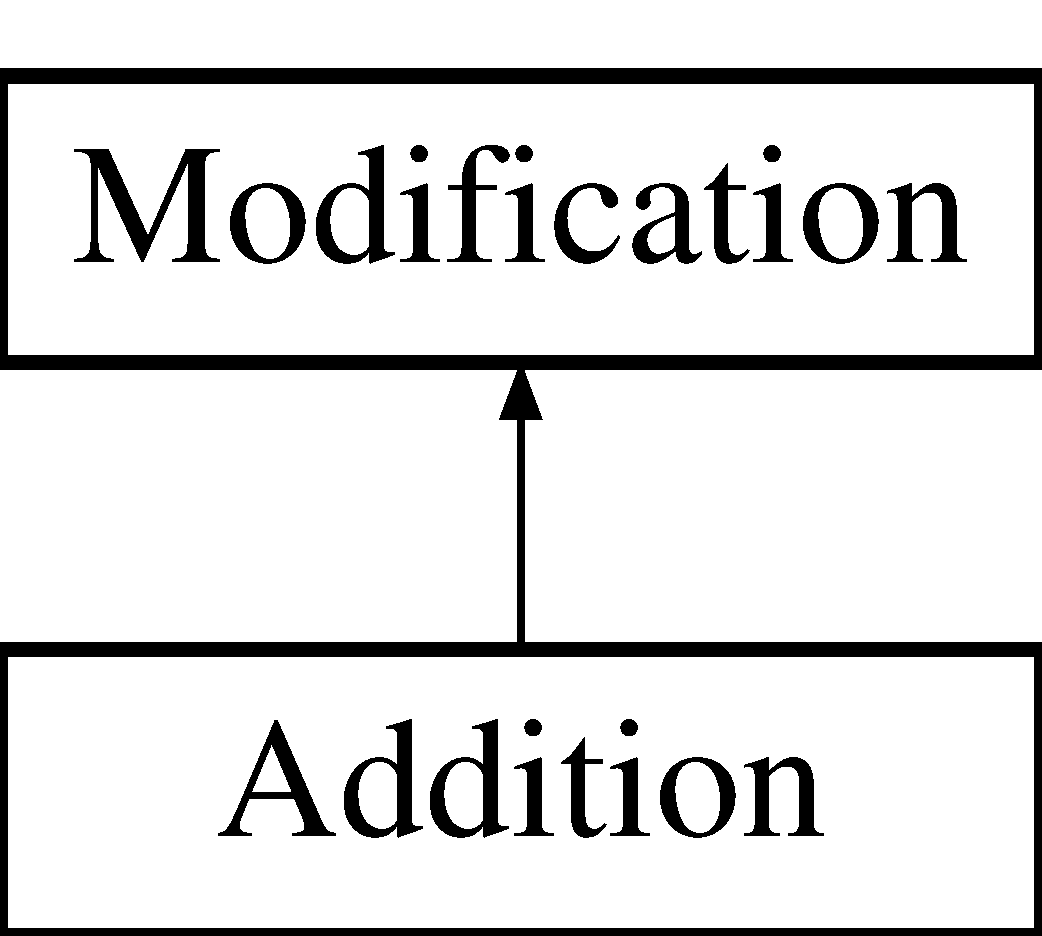
\includegraphics[height=2.000000cm]{classAddition}
\end{center}
\end{figure}
\subsection*{Public Member Functions}
\begin{DoxyCompactItemize}
\item 
\mbox{\Hypertarget{classAddition_a0bcd6cd605c0e90a834339a1feb20901}\label{classAddition_a0bcd6cd605c0e90a834339a1feb20901}} 
{\bfseries Addition} (\mbox{\hyperlink{classTreeObject}{Tree\+Object}} $\ast$obj, \mbox{\hyperlink{classTreeObject}{Tree\+Object}} $\ast$parent)
\item 
\mbox{\Hypertarget{classAddition_acbbe0d8b7c79cc7cdf95124ce834553c}\label{classAddition_acbbe0d8b7c79cc7cdf95124ce834553c}} 
void {\bfseries write\+Out} (\mbox{\hyperlink{classPartitionManager}{Partition\+Manager}} $\ast$pm)
\end{DoxyCompactItemize}
\subsection*{Additional Inherited Members}


The documentation for this class was generated from the following files\+:\begin{DoxyCompactItemize}
\item 
Trees.\+h\item 
Trees.\+cpp\end{DoxyCompactItemize}

\hypertarget{classarboreal__cli__error}{}\section{arboreal\+\_\+cli\+\_\+error Class Reference}
\label{classarboreal__cli__error}\index{arboreal\+\_\+cli\+\_\+error@{arboreal\+\_\+cli\+\_\+error}}
Inheritance diagram for arboreal\+\_\+cli\+\_\+error\+:\begin{figure}[H]
\begin{center}
\leavevmode
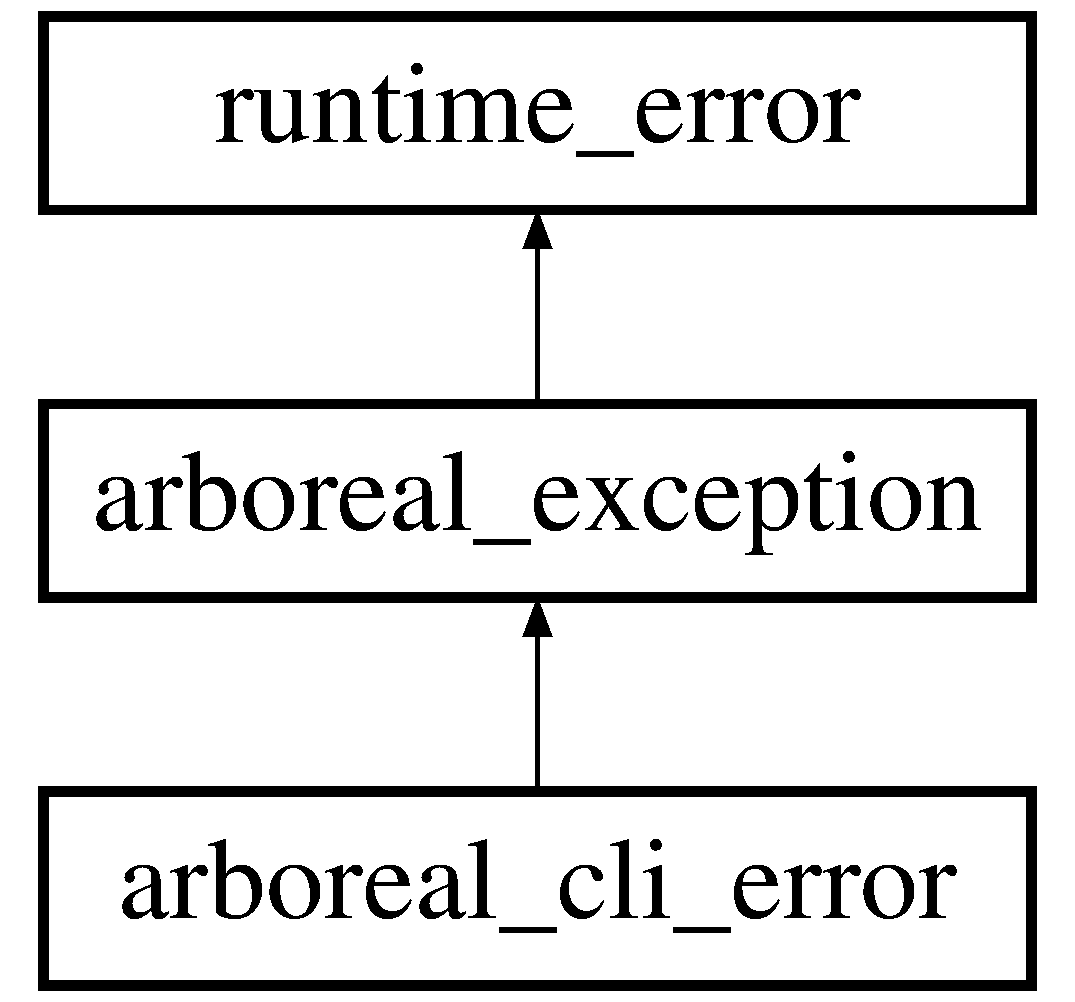
\includegraphics[height=3.000000cm]{d2/d7d/classarboreal__cli__error}
\end{center}
\end{figure}
\subsection*{Public Member Functions}
\begin{DoxyCompactItemize}
\item 
\mbox{\Hypertarget{classarboreal__cli__error_a39291e6c997b531c712892b9623f938a}\label{classarboreal__cli__error_a39291e6c997b531c712892b9623f938a}} 
{\bfseries arboreal\+\_\+cli\+\_\+error} (const string \&where, const string \&what, const int ecode=99)
\item 
\mbox{\Hypertarget{classarboreal__cli__error_adecf3ae0818fcdff4d375ef12ea1659e}\label{classarboreal__cli__error_adecf3ae0818fcdff4d375ef12ea1659e}} 
{\bfseries arboreal\+\_\+cli\+\_\+error} (const char $\ast$what, const char $\ast$where, const int ecode=99)
\item 
\mbox{\Hypertarget{classarboreal__cli__error_ab9388ea7e89c5232d7dd43d00019fef6}\label{classarboreal__cli__error_ab9388ea7e89c5232d7dd43d00019fef6}} 
{\bfseries arboreal\+\_\+cli\+\_\+error} (const char $\ast$what, const string \&where, const int ecode=99)
\item 
\mbox{\Hypertarget{classarboreal__cli__error_a297adfc95de15ebdceae7cf364d05600}\label{classarboreal__cli__error_a297adfc95de15ebdceae7cf364d05600}} 
{\bfseries arboreal\+\_\+cli\+\_\+error} (const string \&what, const char $\ast$where, const int ecode=99)
\end{DoxyCompactItemize}
\subsection*{Additional Inherited Members}


The documentation for this class was generated from the following files\+:\begin{DoxyCompactItemize}
\item 
Shared\+Headers/Arboreal\+\_\+\+Exceptions.\+h\item 
Shared\+C\+P\+P\+Files/Arboreal\+\_\+\+Exceptions.\+cpp\end{DoxyCompactItemize}

\hypertarget{classarboreal__daemon__error}{}\section{arboreal\+\_\+daemon\+\_\+error Class Reference}
\label{classarboreal__daemon__error}\index{arboreal\+\_\+daemon\+\_\+error@{arboreal\+\_\+daemon\+\_\+error}}
Inheritance diagram for arboreal\+\_\+daemon\+\_\+error\+:\begin{figure}[H]
\begin{center}
\leavevmode
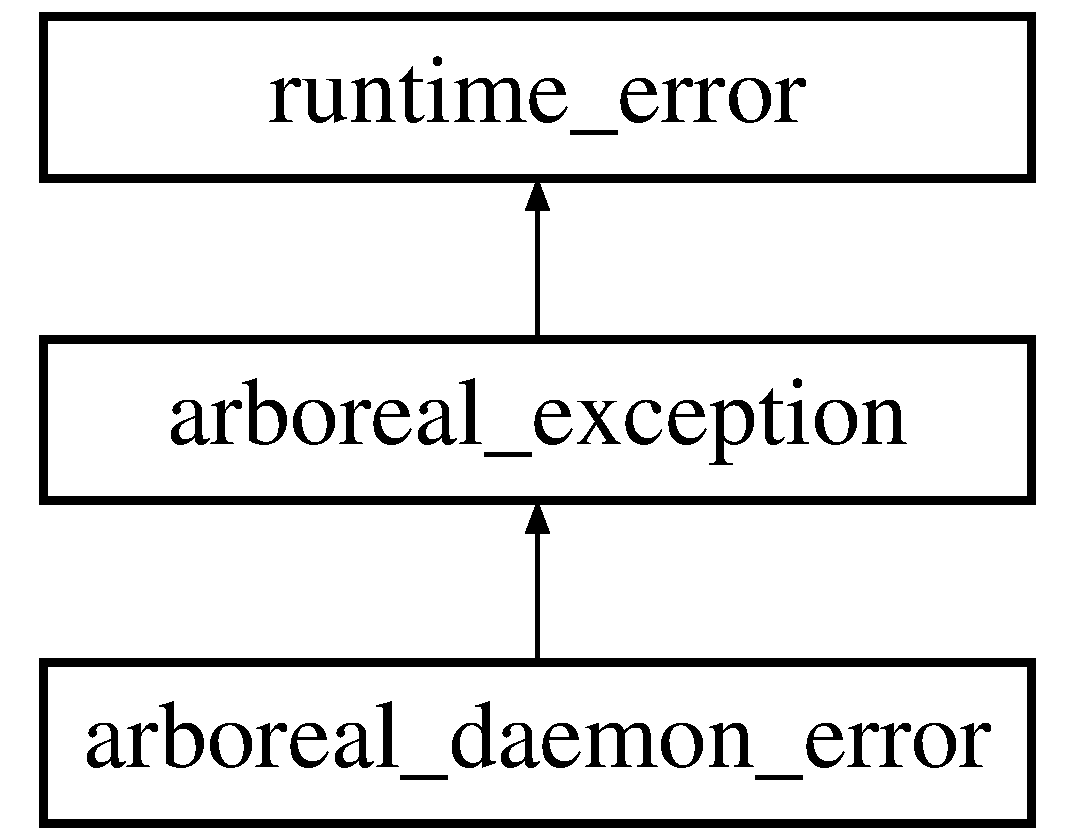
\includegraphics[height=3.000000cm]{db/d0e/classarboreal__daemon__error}
\end{center}
\end{figure}
\subsection*{Public Member Functions}
\begin{DoxyCompactItemize}
\item 
\mbox{\Hypertarget{classarboreal__daemon__error_aaa483ea710b1c20f37a61b7be7cd64fd}\label{classarboreal__daemon__error_aaa483ea710b1c20f37a61b7be7cd64fd}} 
{\bfseries arboreal\+\_\+daemon\+\_\+error} (const string \&where, const string \&what, const int ecode=99)
\item 
\mbox{\Hypertarget{classarboreal__daemon__error_a4a8b88442bf94bf88ffa162c8e8f76ef}\label{classarboreal__daemon__error_a4a8b88442bf94bf88ffa162c8e8f76ef}} 
{\bfseries arboreal\+\_\+daemon\+\_\+error} (const char $\ast$what, const char $\ast$where, const int ecode=99)
\item 
\mbox{\Hypertarget{classarboreal__daemon__error_a32d6c4b31f97c709952f44e15fd6bf8a}\label{classarboreal__daemon__error_a32d6c4b31f97c709952f44e15fd6bf8a}} 
{\bfseries arboreal\+\_\+daemon\+\_\+error} (const char $\ast$what, const string \&where, const int ecode=99)
\item 
\mbox{\Hypertarget{classarboreal__daemon__error_adc8e08526e65a9707c55b674c8d02044}\label{classarboreal__daemon__error_adc8e08526e65a9707c55b674c8d02044}} 
{\bfseries arboreal\+\_\+daemon\+\_\+error} (const string \&what, const char $\ast$where, const int ecode=99)
\end{DoxyCompactItemize}
\subsection*{Additional Inherited Members}


The documentation for this class was generated from the following files\+:\begin{DoxyCompactItemize}
\item 
Shared\+Headers/Arboreal\+\_\+\+Exceptions.\+h\item 
Shared\+C\+P\+P\+Files/Arboreal\+\_\+\+Exceptions.\+cpp\end{DoxyCompactItemize}

\hypertarget{classarboreal__exception}{}\section{arboreal\+\_\+exception Class Reference}
\label{classarboreal__exception}\index{arboreal\+\_\+exception@{arboreal\+\_\+exception}}
Inheritance diagram for arboreal\+\_\+exception\+:\begin{figure}[H]
\begin{center}
\leavevmode
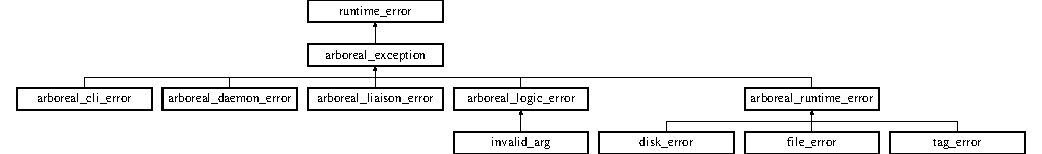
\includegraphics[height=3.684211cm]{classarboreal__exception}
\end{center}
\end{figure}
\subsection*{Public Member Functions}
\begin{DoxyCompactItemize}
\item 
\mbox{\Hypertarget{classarboreal__exception_a45ed8be47f52411504834440c481bc5f}\label{classarboreal__exception_a45ed8be47f52411504834440c481bc5f}} 
{\bfseries arboreal\+\_\+exception} (const char $\ast$what, const char $\ast$where)
\item 
\mbox{\Hypertarget{classarboreal__exception_a7d89267e972d47ac4052e3d6c94ee73b}\label{classarboreal__exception_a7d89267e972d47ac4052e3d6c94ee73b}} 
{\bfseries arboreal\+\_\+exception} (const char $\ast$what, const string \&where)
\item 
\mbox{\Hypertarget{classarboreal__exception_a3a3f2a7034c07dc5fe694ff860c0d4b4}\label{classarboreal__exception_a3a3f2a7034c07dc5fe694ff860c0d4b4}} 
{\bfseries arboreal\+\_\+exception} (const string \&what, const string \&where)
\item 
\mbox{\Hypertarget{classarboreal__exception_ac3099afc0a14eed3408dfffaac47d4ca}\label{classarboreal__exception_ac3099afc0a14eed3408dfffaac47d4ca}} 
{\bfseries arboreal\+\_\+exception} (const string \&what, const char $\ast$where)
\item 
\mbox{\Hypertarget{classarboreal__exception_a802003dee586aaeb0b0d7ce909da2dad}\label{classarboreal__exception_a802003dee586aaeb0b0d7ce909da2dad}} 
virtual const char $\ast$ {\bfseries where} () const
\end{DoxyCompactItemize}
\subsection*{Protected Attributes}
\begin{DoxyCompactItemize}
\item 
\mbox{\Hypertarget{classarboreal__exception_a73559e45af28b0804b66b04df4c04270}\label{classarboreal__exception_a73559e45af28b0804b66b04df4c04270}} 
string {\bfseries \+\_\+where}
\end{DoxyCompactItemize}


The documentation for this class was generated from the following files\+:\begin{DoxyCompactItemize}
\item 
Arboreal\+\_\+\+Exceptions.\+h\item 
Arboreal\+\_\+\+Exceptions.\+cpp\end{DoxyCompactItemize}

\hypertarget{classarboreal__liaison__error}{}\section{arboreal\+\_\+liaison\+\_\+error Class Reference}
\label{classarboreal__liaison__error}\index{arboreal\+\_\+liaison\+\_\+error@{arboreal\+\_\+liaison\+\_\+error}}
Inheritance diagram for arboreal\+\_\+liaison\+\_\+error\+:\begin{figure}[H]
\begin{center}
\leavevmode
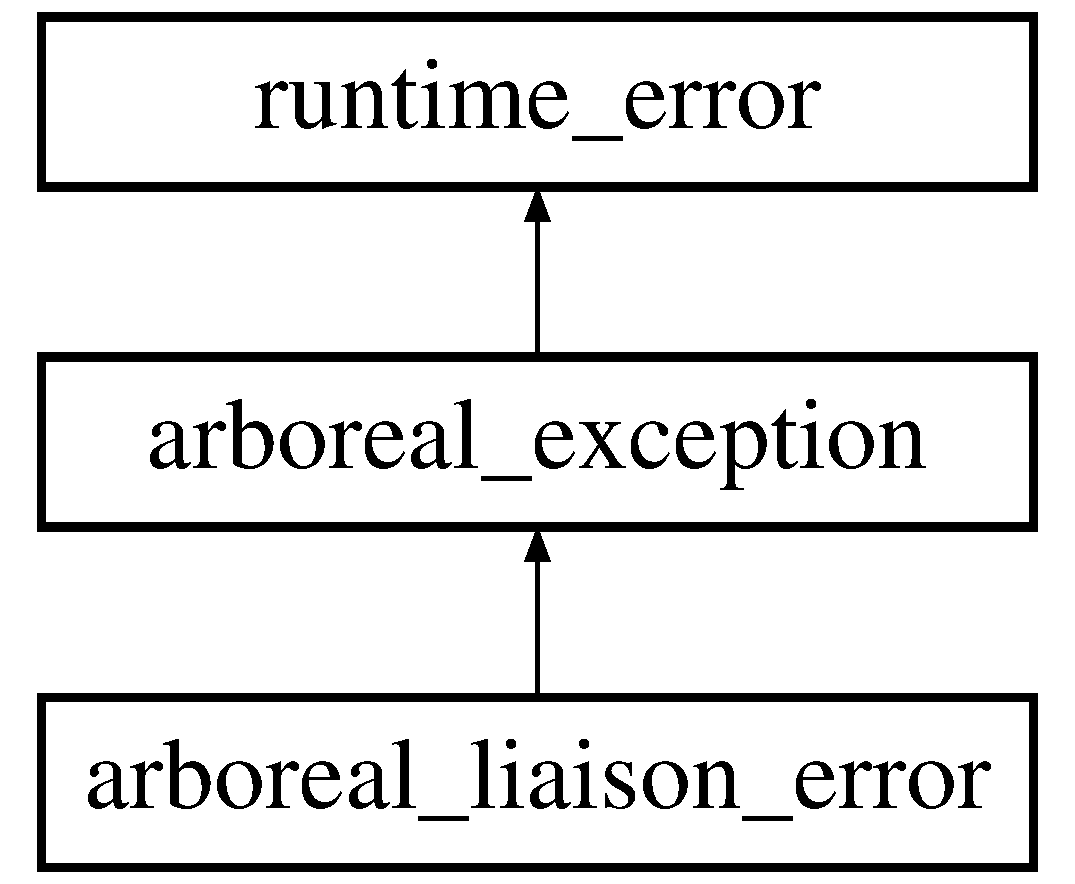
\includegraphics[height=3.000000cm]{classarboreal__liaison__error}
\end{center}
\end{figure}
\subsection*{Public Member Functions}
\begin{DoxyCompactItemize}
\item 
{\bfseries arboreal\+\_\+liaison\+\_\+error} (const string \&where, const string \&what, const int ecode=99)\hypertarget{classarboreal__liaison__error_af23c4a3672c9594e3382a05a1590abc4}{}\label{classarboreal__liaison__error_af23c4a3672c9594e3382a05a1590abc4}

\item 
{\bfseries arboreal\+\_\+liaison\+\_\+error} (const char $\ast$what, const char $\ast$where, const int ecode=99)\hypertarget{classarboreal__liaison__error_ae9eaf00df34e37262348e254c6dad5ff}{}\label{classarboreal__liaison__error_ae9eaf00df34e37262348e254c6dad5ff}

\item 
{\bfseries arboreal\+\_\+liaison\+\_\+error} (const char $\ast$what, const string \&where, const int ecode=99)\hypertarget{classarboreal__liaison__error_a593436824d649179f5c34b7311c56d2e}{}\label{classarboreal__liaison__error_a593436824d649179f5c34b7311c56d2e}

\item 
{\bfseries arboreal\+\_\+liaison\+\_\+error} (const string \&what, const char $\ast$where, const int ecode=99)\hypertarget{classarboreal__liaison__error_a73221c813d25af214f19eaec704ffffd}{}\label{classarboreal__liaison__error_a73221c813d25af214f19eaec704ffffd}

\end{DoxyCompactItemize}
\subsection*{Additional Inherited Members}


The documentation for this class was generated from the following files\+:\begin{DoxyCompactItemize}
\item 
Shared\+Headers/Arboreal\+\_\+\+Exceptions.\+h\item 
Shared\+C\+P\+P\+Files/Arboreal\+\_\+\+Exceptions.\+cpp\end{DoxyCompactItemize}

\hypertarget{classarboreal__logic__error}{}\section{arboreal\+\_\+logic\+\_\+error Class Reference}
\label{classarboreal__logic__error}\index{arboreal\+\_\+logic\+\_\+error@{arboreal\+\_\+logic\+\_\+error}}
Inheritance diagram for arboreal\+\_\+logic\+\_\+error\+:\begin{figure}[H]
\begin{center}
\leavevmode
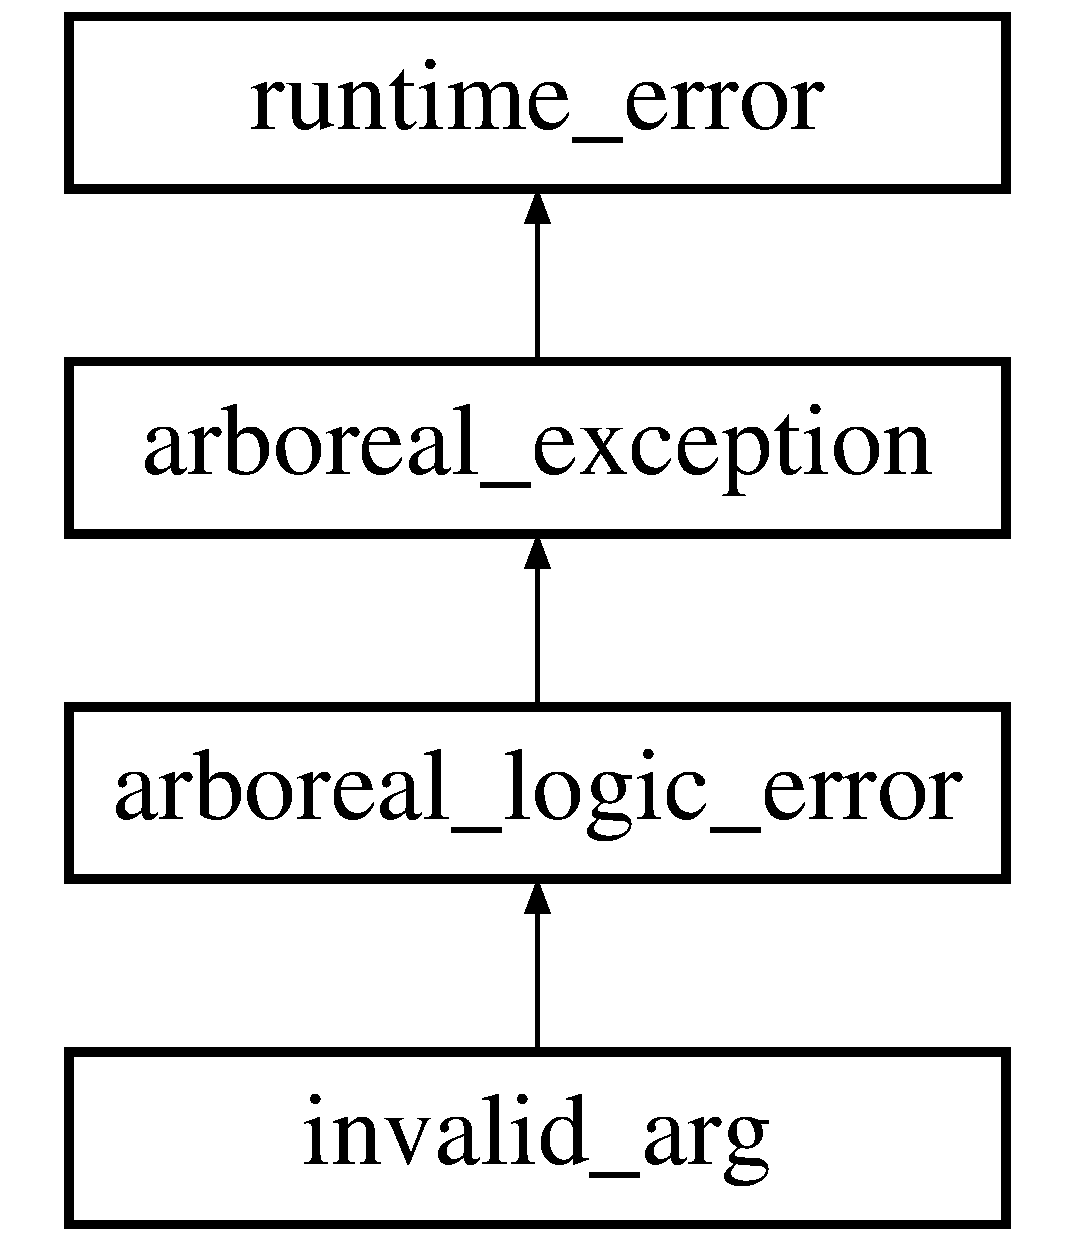
\includegraphics[height=4.000000cm]{classarboreal__logic__error}
\end{center}
\end{figure}
\subsection*{Public Member Functions}
\begin{DoxyCompactItemize}
\item 
{\bfseries arboreal\+\_\+logic\+\_\+error} (const char $\ast$what, const char $\ast$where, const int ecode=99)\hypertarget{classarboreal__logic__error_aaea786c69fe107f9b6753b51001c59d6}{}\label{classarboreal__logic__error_aaea786c69fe107f9b6753b51001c59d6}

\item 
{\bfseries arboreal\+\_\+logic\+\_\+error} (const char $\ast$what, const string \&where, const int ecode=99)\hypertarget{classarboreal__logic__error_a70b8217c9841efc9bb1e556282a89fe0}{}\label{classarboreal__logic__error_a70b8217c9841efc9bb1e556282a89fe0}

\item 
{\bfseries arboreal\+\_\+logic\+\_\+error} (const string \&what, const string \&where, const int ecode=99)\hypertarget{classarboreal__logic__error_ad7627c19a966b137cf018aa7c3075421}{}\label{classarboreal__logic__error_ad7627c19a966b137cf018aa7c3075421}

\item 
{\bfseries arboreal\+\_\+logic\+\_\+error} (const string \&what, const char $\ast$where, const int ecode=99)\hypertarget{classarboreal__logic__error_a5c589df18299902a24dae25f8a25c02a}{}\label{classarboreal__logic__error_a5c589df18299902a24dae25f8a25c02a}

\end{DoxyCompactItemize}
\subsection*{Additional Inherited Members}


The documentation for this class was generated from the following files\+:\begin{DoxyCompactItemize}
\item 
Shared\+Headers/Arboreal\+\_\+\+Exceptions.\+h\item 
Shared\+C\+P\+P\+Files/Arboreal\+\_\+\+Exceptions.\+cpp\end{DoxyCompactItemize}

\hypertarget{classarboreal__runtime__error}{}\section{arboreal\+\_\+runtime\+\_\+error Class Reference}
\label{classarboreal__runtime__error}\index{arboreal\+\_\+runtime\+\_\+error@{arboreal\+\_\+runtime\+\_\+error}}
Inheritance diagram for arboreal\+\_\+runtime\+\_\+error\+:\begin{figure}[H]
\begin{center}
\leavevmode
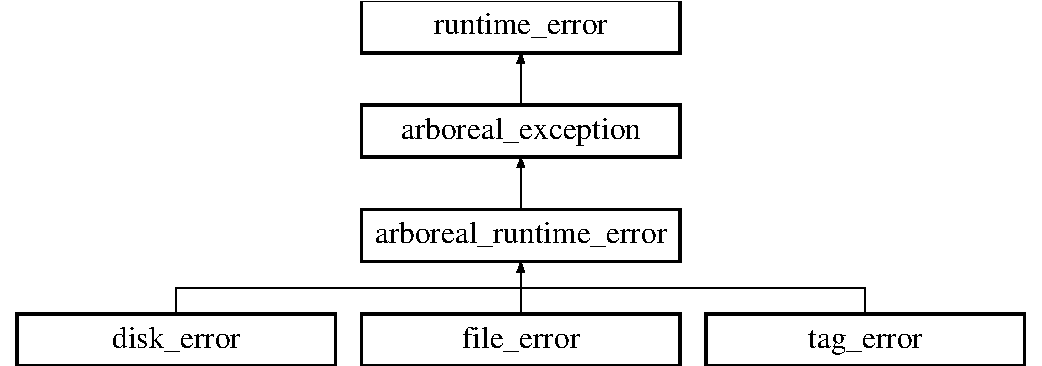
\includegraphics[height=4.000000cm]{classarboreal__runtime__error}
\end{center}
\end{figure}
\subsection*{Public Member Functions}
\begin{DoxyCompactItemize}
\item 
{\bfseries arboreal\+\_\+runtime\+\_\+error} (const char $\ast$what, const char $\ast$where, const int ecode=99)\hypertarget{classarboreal__runtime__error_aa6970966b569a105ead4fc6a5648cb5e}{}\label{classarboreal__runtime__error_aa6970966b569a105ead4fc6a5648cb5e}

\item 
{\bfseries arboreal\+\_\+runtime\+\_\+error} (const char $\ast$what, const string \&where, const int ecode=99)\hypertarget{classarboreal__runtime__error_af20cdd8f990b40293bbbf11f3fe1005b}{}\label{classarboreal__runtime__error_af20cdd8f990b40293bbbf11f3fe1005b}

\item 
{\bfseries arboreal\+\_\+runtime\+\_\+error} (const string \&what, const string \&where, const int ecode=99)\hypertarget{classarboreal__runtime__error_a3797d6f9ba8c5590539b280042d023a5}{}\label{classarboreal__runtime__error_a3797d6f9ba8c5590539b280042d023a5}

\item 
{\bfseries arboreal\+\_\+runtime\+\_\+error} (const string \&what, const char $\ast$where, const int ecode=99)\hypertarget{classarboreal__runtime__error_a897b94adcbe8bdbcd8c7299d95c4e020}{}\label{classarboreal__runtime__error_a897b94adcbe8bdbcd8c7299d95c4e020}

\end{DoxyCompactItemize}
\subsection*{Protected Attributes}
\begin{DoxyCompactItemize}
\item 
string {\bfseries \+\_\+where}\hypertarget{classarboreal__runtime__error_afca0adf6a259600843b6975591e0bde4}{}\label{classarboreal__runtime__error_afca0adf6a259600843b6975591e0bde4}

\item 
int {\bfseries \+\_\+ecode}\hypertarget{classarboreal__runtime__error_a08953e7ed35ac7db0d86032a3eb3f837}{}\label{classarboreal__runtime__error_a08953e7ed35ac7db0d86032a3eb3f837}

\end{DoxyCompactItemize}


The documentation for this class was generated from the following files\+:\begin{DoxyCompactItemize}
\item 
Shared\+Headers/Arboreal\+\_\+\+Exceptions.\+h\item 
Shared\+C\+P\+P\+Files/Arboreal\+\_\+\+Exceptions.\+cpp\end{DoxyCompactItemize}

\hypertarget{classAttributes}{}\section{Attributes Class Reference}
\label{classAttributes}\index{Attributes@{Attributes}}
\subsection*{Public Member Functions}
\begin{DoxyCompactItemize}
\item 
\mbox{\Hypertarget{classAttributes_a0d6b154029e34f811f0930806768f022}\label{classAttributes_a0d6b154029e34f811f0930806768f022}} 
{\bfseries Attributes} (Blk\+Num\+Type blknum, \mbox{\hyperlink{classPartitionManager}{Partition\+Manager}} $\ast$pm)
\end{DoxyCompactItemize}
\begin{Indent}\textbf{ Modifier Functions}\par
\begin{DoxyCompactItemize}
\item 
void \mbox{\hyperlink{classAttributes_a7eea700dd80e77a74afdc3c091a178b8}{write\+Out}} ()
\item 
void \mbox{\hyperlink{classAttributes_a6fc0012ff20912b8ee30167fefd1ab85}{read\+In}} ()
\item 
void \mbox{\hyperlink{classAttributes_acf28e724c914f066ecdae788d95b3212}{del}} ()
\item 
void \mbox{\hyperlink{classAttributes_a4caf96b812e181975045a172fe0dc438}{set\+Creation\+Time}} ()
\item 
void \mbox{\hyperlink{classAttributes_a56ab60c4bad40e1a47e096526f3ce57a}{set\+Owner}} (int owner)
\item 
void \mbox{\hyperlink{classAttributes_a15a4348203635ff53a6cd8c2d52c68e3}{set\+Permissions}} (char $\ast$perms)
\item 
void \mbox{\hyperlink{classAttributes_ae4861b7312f8619a6b2988b9456c4604}{set\+Access}} ()
\item 
void \mbox{\hyperlink{classAttributes_aa091d2dba315a124ea4a14308f2553c6}{set\+Edit}} ()
\item 
void \mbox{\hyperlink{classAttributes_a6ed2adf53cd6131c2b22a2782cd0bdcf}{update\+Size}} (size\+\_\+t size)
\end{DoxyCompactItemize}
\end{Indent}
\begin{Indent}\textbf{ Accessor Functions}\par
\begin{DoxyCompactItemize}
\item 
time\+\_\+t \mbox{\hyperlink{classAttributes_ac6436c08d31dfa33783feee3469a88e9}{get\+Creation\+Time}} ()
\item 
int \mbox{\hyperlink{classAttributes_a378205f2087ee66d95eb58aa5d7fb040}{get\+Owner}} ()
\item 
char $\ast$ \mbox{\hyperlink{classAttributes_af538b17bd7a459f4664446c574d83bd5}{get\+Permissions}} ()
\item 
time\+\_\+t \mbox{\hyperlink{classAttributes_a1b366a9e556ab09004064f23e84f6fcb}{get\+Access}} ()
\item 
time\+\_\+t \mbox{\hyperlink{classAttributes_a7b646531a3cb941912802eed0ef91f54}{get\+Edit}} ()
\item 
size\+\_\+t \mbox{\hyperlink{classAttributes_af9970a8e76e48221ec9d7832e1e558a3}{get\+Size}} ()
\end{DoxyCompactItemize}
\end{Indent}


\subsection{Member Function Documentation}
\mbox{\Hypertarget{classAttributes_acf28e724c914f066ecdae788d95b3212}\label{classAttributes_acf28e724c914f066ecdae788d95b3212}} 
\index{Attributes@{Attributes}!del@{del}}
\index{del@{del}!Attributes@{Attributes}}
\subsubsection{\texorpdfstring{del()}{del()}}
{\footnotesize\ttfamily void Attributes\+::del (\begin{DoxyParamCaption}{ }\end{DoxyParamCaption})}

Removes the \mbox{\hyperlink{classAttributes}{Attributes}} presence on disk \mbox{\Hypertarget{classAttributes_a1b366a9e556ab09004064f23e84f6fcb}\label{classAttributes_a1b366a9e556ab09004064f23e84f6fcb}} 
\index{Attributes@{Attributes}!get\+Access@{get\+Access}}
\index{get\+Access@{get\+Access}!Attributes@{Attributes}}
\subsubsection{\texorpdfstring{get\+Access()}{getAccess()}}
{\footnotesize\ttfamily time\+\_\+t Attributes\+::get\+Access (\begin{DoxyParamCaption}{ }\end{DoxyParamCaption})}

\begin{DoxyReturn}{Returns}
the U\+N\+IX time the file was last accessed 
\end{DoxyReturn}
\mbox{\Hypertarget{classAttributes_ac6436c08d31dfa33783feee3469a88e9}\label{classAttributes_ac6436c08d31dfa33783feee3469a88e9}} 
\index{Attributes@{Attributes}!get\+Creation\+Time@{get\+Creation\+Time}}
\index{get\+Creation\+Time@{get\+Creation\+Time}!Attributes@{Attributes}}
\subsubsection{\texorpdfstring{get\+Creation\+Time()}{getCreationTime()}}
{\footnotesize\ttfamily time\+\_\+t Attributes\+::get\+Creation\+Time (\begin{DoxyParamCaption}{ }\end{DoxyParamCaption})}

\begin{DoxyReturn}{Returns}
the U\+N\+IX time the file was created 
\end{DoxyReturn}
\mbox{\Hypertarget{classAttributes_a7b646531a3cb941912802eed0ef91f54}\label{classAttributes_a7b646531a3cb941912802eed0ef91f54}} 
\index{Attributes@{Attributes}!get\+Edit@{get\+Edit}}
\index{get\+Edit@{get\+Edit}!Attributes@{Attributes}}
\subsubsection{\texorpdfstring{get\+Edit()}{getEdit()}}
{\footnotesize\ttfamily time\+\_\+t Attributes\+::get\+Edit (\begin{DoxyParamCaption}{ }\end{DoxyParamCaption})}

\begin{DoxyReturn}{Returns}
the U\+N\+IX time the file was last edited 
\end{DoxyReturn}
\mbox{\Hypertarget{classAttributes_a378205f2087ee66d95eb58aa5d7fb040}\label{classAttributes_a378205f2087ee66d95eb58aa5d7fb040}} 
\index{Attributes@{Attributes}!get\+Owner@{get\+Owner}}
\index{get\+Owner@{get\+Owner}!Attributes@{Attributes}}
\subsubsection{\texorpdfstring{get\+Owner()}{getOwner()}}
{\footnotesize\ttfamily int Attributes\+::get\+Owner (\begin{DoxyParamCaption}{ }\end{DoxyParamCaption})}

\begin{DoxyReturn}{Returns}
the U\+ID of the owner of the file 
\end{DoxyReturn}
\mbox{\Hypertarget{classAttributes_af538b17bd7a459f4664446c574d83bd5}\label{classAttributes_af538b17bd7a459f4664446c574d83bd5}} 
\index{Attributes@{Attributes}!get\+Permissions@{get\+Permissions}}
\index{get\+Permissions@{get\+Permissions}!Attributes@{Attributes}}
\subsubsection{\texorpdfstring{get\+Permissions()}{getPermissions()}}
{\footnotesize\ttfamily char $\ast$ Attributes\+::get\+Permissions (\begin{DoxyParamCaption}{ }\end{DoxyParamCaption})}

\begin{DoxyReturn}{Returns}
the permisssions 
\end{DoxyReturn}
\begin{DoxySeeAlso}{See also}
File\+Info\+::get\+Permissions(char$\ast$) 
\end{DoxySeeAlso}
\mbox{\Hypertarget{classAttributes_af9970a8e76e48221ec9d7832e1e558a3}\label{classAttributes_af9970a8e76e48221ec9d7832e1e558a3}} 
\index{Attributes@{Attributes}!get\+Size@{get\+Size}}
\index{get\+Size@{get\+Size}!Attributes@{Attributes}}
\subsubsection{\texorpdfstring{get\+Size()}{getSize()}}
{\footnotesize\ttfamily size\+\_\+t Attributes\+::get\+Size (\begin{DoxyParamCaption}{ }\end{DoxyParamCaption})}

\begin{DoxyReturn}{Returns}
the size of the file in bytes 
\end{DoxyReturn}
\mbox{\Hypertarget{classAttributes_a6fc0012ff20912b8ee30167fefd1ab85}\label{classAttributes_a6fc0012ff20912b8ee30167fefd1ab85}} 
\index{Attributes@{Attributes}!read\+In@{read\+In}}
\index{read\+In@{read\+In}!Attributes@{Attributes}}
\subsubsection{\texorpdfstring{read\+In()}{readIn()}}
{\footnotesize\ttfamily void Attributes\+::read\+In (\begin{DoxyParamCaption}{ }\end{DoxyParamCaption})}

Reads in the \mbox{\hyperlink{classAttributes}{Attributes}} from disk \mbox{\Hypertarget{classAttributes_ae4861b7312f8619a6b2988b9456c4604}\label{classAttributes_ae4861b7312f8619a6b2988b9456c4604}} 
\index{Attributes@{Attributes}!set\+Access@{set\+Access}}
\index{set\+Access@{set\+Access}!Attributes@{Attributes}}
\subsubsection{\texorpdfstring{set\+Access()}{setAccess()}}
{\footnotesize\ttfamily void Attributes\+::set\+Access (\begin{DoxyParamCaption}{ }\end{DoxyParamCaption})}

Marks down the time as accessed time as U\+N\+IX timestamp \mbox{\Hypertarget{classAttributes_a4caf96b812e181975045a172fe0dc438}\label{classAttributes_a4caf96b812e181975045a172fe0dc438}} 
\index{Attributes@{Attributes}!set\+Creation\+Time@{set\+Creation\+Time}}
\index{set\+Creation\+Time@{set\+Creation\+Time}!Attributes@{Attributes}}
\subsubsection{\texorpdfstring{set\+Creation\+Time()}{setCreationTime()}}
{\footnotesize\ttfamily void Attributes\+::set\+Creation\+Time (\begin{DoxyParamCaption}{ }\end{DoxyParamCaption})}

Marks down the creation time of the associated \mbox{\hyperlink{classFileInfo}{File\+Info}} as U\+N\+IX timestamp \mbox{\Hypertarget{classAttributes_aa091d2dba315a124ea4a14308f2553c6}\label{classAttributes_aa091d2dba315a124ea4a14308f2553c6}} 
\index{Attributes@{Attributes}!set\+Edit@{set\+Edit}}
\index{set\+Edit@{set\+Edit}!Attributes@{Attributes}}
\subsubsection{\texorpdfstring{set\+Edit()}{setEdit()}}
{\footnotesize\ttfamily void Attributes\+::set\+Edit (\begin{DoxyParamCaption}{ }\end{DoxyParamCaption})}

Marks down the time as modified time as U\+N\+IX timestamp \mbox{\Hypertarget{classAttributes_a56ab60c4bad40e1a47e096526f3ce57a}\label{classAttributes_a56ab60c4bad40e1a47e096526f3ce57a}} 
\index{Attributes@{Attributes}!set\+Owner@{set\+Owner}}
\index{set\+Owner@{set\+Owner}!Attributes@{Attributes}}
\subsubsection{\texorpdfstring{set\+Owner()}{setOwner()}}
{\footnotesize\ttfamily void Attributes\+::set\+Owner (\begin{DoxyParamCaption}\item[{int}]{owner }\end{DoxyParamCaption})}

Marks the owner as their U\+ID \mbox{\Hypertarget{classAttributes_a15a4348203635ff53a6cd8c2d52c68e3}\label{classAttributes_a15a4348203635ff53a6cd8c2d52c68e3}} 
\index{Attributes@{Attributes}!set\+Permissions@{set\+Permissions}}
\index{set\+Permissions@{set\+Permissions}!Attributes@{Attributes}}
\subsubsection{\texorpdfstring{set\+Permissions()}{setPermissions()}}
{\footnotesize\ttfamily void Attributes\+::set\+Permissions (\begin{DoxyParamCaption}\item[{char $\ast$}]{perms }\end{DoxyParamCaption})}

sets the permisssions of the file \begin{DoxySeeAlso}{See also}
\mbox{\hyperlink{classFileInfo_ab2b69861ecef1b8e0f465906c8eaa7a7}{File\+Info\+::set\+Permissions(char$\ast$)}} 
\end{DoxySeeAlso}
\mbox{\Hypertarget{classAttributes_a6ed2adf53cd6131c2b22a2782cd0bdcf}\label{classAttributes_a6ed2adf53cd6131c2b22a2782cd0bdcf}} 
\index{Attributes@{Attributes}!update\+Size@{update\+Size}}
\index{update\+Size@{update\+Size}!Attributes@{Attributes}}
\subsubsection{\texorpdfstring{update\+Size()}{updateSize()}}
{\footnotesize\ttfamily void Attributes\+::update\+Size (\begin{DoxyParamCaption}\item[{size\+\_\+t}]{size }\end{DoxyParamCaption})}

sets the size to the specified size \mbox{\Hypertarget{classAttributes_a7eea700dd80e77a74afdc3c091a178b8}\label{classAttributes_a7eea700dd80e77a74afdc3c091a178b8}} 
\index{Attributes@{Attributes}!write\+Out@{write\+Out}}
\index{write\+Out@{write\+Out}!Attributes@{Attributes}}
\subsubsection{\texorpdfstring{write\+Out()}{writeOut()}}
{\footnotesize\ttfamily void Attributes\+::write\+Out (\begin{DoxyParamCaption}{ }\end{DoxyParamCaption})}

Writes out the \mbox{\hyperlink{classAttributes}{Attributes}} to disk 

The documentation for this class was generated from the following files\+:\begin{DoxyCompactItemize}
\item 
Trees.\+h\item 
Trees.\+cpp\end{DoxyCompactItemize}

\hypertarget{classCLI}{}\section{C\+LI Class Reference}
\label{classCLI}\index{C\+LI@{C\+LI}}
\subsection*{Public Member Functions}
\begin{DoxyCompactItemize}
\item 
\mbox{\Hypertarget{classCLI_a0c3b5662a3f33b5a76021be177c3eef2}\label{classCLI_a0c3b5662a3f33b5a76021be177c3eef2}} 
{\bfseries C\+LI} (char $\ast$$\ast$partition)
\item 
\mbox{\Hypertarget{classCLI_aeafaa56f2b2d8c97121ed52125e3fa9a}\label{classCLI_aeafaa56f2b2d8c97121ed52125e3fa9a}} 
{\bfseries C\+LI} (char $\ast$$\ast$partition, bool debug)
\item 
\mbox{\Hypertarget{classCLI_a4eb5e9a1c695edf4dcc705b9c12a0a8d}\label{classCLI_a4eb5e9a1c695edf4dcc705b9c12a0a8d}} 
{\bfseries C\+LI} (char $\ast$$\ast$partition, char $\ast$is\+Script)
\item 
\mbox{\Hypertarget{classCLI_a5d9746160fc642addd9b4aff6cc4eef2}\label{classCLI_a5d9746160fc642addd9b4aff6cc4eef2}} 
{\bfseries C\+LI} (char $\ast$$\ast$partition, char $\ast$is\+Script, bool debug)
\item 
\mbox{\Hypertarget{classCLI_a1492005f186392031bd4d447cb20e975}\label{classCLI_a1492005f186392031bd4d447cb20e975}} 
void {\bfseries start} ()
\item 
\mbox{\Hypertarget{classCLI_a5ce3ce0818fc0afe2a277995000ea22b}\label{classCLI_a5ce3ce0818fc0afe2a277995000ea22b}} 
void {\bfseries run} (std\+::string input)
\item 
\mbox{\Hypertarget{classCLI_aeefc8cd81999836a90c2cfaced6177f1}\label{classCLI_aeefc8cd81999836a90c2cfaced6177f1}} 
void {\bfseries run} ()
\item 
\mbox{\Hypertarget{classCLI_a2019fb3e1ab4580218d507859883d8dd}\label{classCLI_a2019fb3e1ab4580218d507859883d8dd}} 
char $\ast$ {\bfseries build} (int id, std\+::string input)
\item 
\mbox{\Hypertarget{classCLI_aba5e2a83a3134c959b1d4fb35c6c72b2}\label{classCLI_aba5e2a83a3134c959b1d4fb35c6c72b2}} 
void {\bfseries send\+\_\+cmnd} (char $\ast$command)
\item 
\mbox{\Hypertarget{classCLI_a87c68e5edcb5750d1199839e6b1f843e}\label{classCLI_a87c68e5edcb5750d1199839e6b1f843e}} 
void {\bfseries await\+\_\+response} ()
\end{DoxyCompactItemize}


The documentation for this class was generated from the following files\+:\begin{DoxyCompactItemize}
\item 
cli.\+h\item 
cli.\+cpp\end{DoxyCompactItemize}

\hypertarget{classDebugMessages}{}\section{Debug\+Messages Class Reference}
\label{classDebugMessages}\index{Debug\+Messages@{Debug\+Messages}}
\subsection*{Public Member Functions}
\begin{DoxyCompactItemize}
\item 
\hyperlink{classDebugMessages_a7fb2c5a7cce97eb05661b1f6657cb650}{Debug\+Messages} ()
\item 
\hyperlink{classDebugMessages_aa60430ca0e05e43a8bb27f4cdc1a158c}{Debug\+Messages} (std\+::string logfile\+\_\+name)
\item 
\hyperlink{classDebugMessages_a3700e476ad70d27ba14be67b43ff6f69}{$\sim$\+Debug\+Messages} ()
\item 
void \hyperlink{classDebugMessages_a95866775dcf301773daa7bed529c557e}{ON} (void)
\item 
void \hyperlink{classDebugMessages_ac1e4085ade0d1ff7b603fd8205f74b7c}{O\+FF} (void)
\item 
{\footnotesize template$<$typename T $>$ }\\void \hyperlink{classDebugMessages_a09343725fb16b9e9d3c5587880e8401e}{display} (const T data, bool force=false)
\item 
{\footnotesize template$<$typename T $>$ }\\void \hyperlink{classDebugMessages_a6b7e8eb509b3d0903e918ae25dec18aa}{log} (const T data, bool force=false)
\item 
{\footnotesize template$<$typename T $>$ }\\void \hyperlink{classDebugMessages_aac71fdadaf41ce9a3dd7dd502096fb51}{debug} (const T data, bool force=false)
\item 
void {\bfseries lock} ()\hypertarget{classDebugMessages_abb8c29cf2e650f04b45edf0087b47d81}{}\label{classDebugMessages_abb8c29cf2e650f04b45edf0087b47d81}

\item 
void {\bfseries unlock} ()\hypertarget{classDebugMessages_a575b874fbfdadaf91eaa7ec4599c78e3}{}\label{classDebugMessages_a575b874fbfdadaf91eaa7ec4599c78e3}

\end{DoxyCompactItemize}


\subsection{Constructor \& Destructor Documentation}
\index{Debug\+Messages@{Debug\+Messages}!Debug\+Messages@{Debug\+Messages}}
\index{Debug\+Messages@{Debug\+Messages}!Debug\+Messages@{Debug\+Messages}}
\subsubsection[{\texorpdfstring{Debug\+Messages()}{DebugMessages()}}]{\setlength{\rightskip}{0pt plus 5cm}Debug\+Messages\+::\+Debug\+Messages (
\begin{DoxyParamCaption}
{}
\end{DoxyParamCaption}
)\hspace{0.3cm}{\ttfamily [inline]}}\hypertarget{classDebugMessages_a7fb2c5a7cce97eb05661b1f6657cb650}{}\label{classDebugMessages_a7fb2c5a7cce97eb05661b1f6657cb650}
Create a new Debug\+Message object using default logfile name\+: \textquotesingle{}Arboreal.\+log\textquotesingle{} Automatically creates the log if it does not exist and if it does exist it will overwrite all the data in the log with the empty string. Sets the debug flag \+\_\+\+D\+E\+B\+UG to F\+A\+L\+SE on startup. \index{Debug\+Messages@{Debug\+Messages}!Debug\+Messages@{Debug\+Messages}}
\index{Debug\+Messages@{Debug\+Messages}!Debug\+Messages@{Debug\+Messages}}
\subsubsection[{\texorpdfstring{Debug\+Messages(std\+::string logfile\+\_\+name)}{DebugMessages(std::string logfile_name)}}]{\setlength{\rightskip}{0pt plus 5cm}Debug\+Messages\+::\+Debug\+Messages (
\begin{DoxyParamCaption}
\item[{std\+::string}]{logfile\+\_\+name}
\end{DoxyParamCaption}
)\hspace{0.3cm}{\ttfamily [inline]}}\hypertarget{classDebugMessages_aa60430ca0e05e43a8bb27f4cdc1a158c}{}\label{classDebugMessages_aa60430ca0e05e43a8bb27f4cdc1a158c}
Create a new Debug\+Message object using a user defined logfile name. Automatically creates the log if it does not exist and if it does exist it will overwrite all the data in the log with the empty string. Sets the debug flag \+\_\+\+D\+E\+B\+UG to F\+A\+L\+SE on startup. \index{Debug\+Messages@{Debug\+Messages}!````~Debug\+Messages@{$\sim$\+Debug\+Messages}}
\index{````~Debug\+Messages@{$\sim$\+Debug\+Messages}!Debug\+Messages@{Debug\+Messages}}
\subsubsection[{\texorpdfstring{$\sim$\+Debug\+Messages()}{~DebugMessages()}}]{\setlength{\rightskip}{0pt plus 5cm}Debug\+Messages\+::$\sim$\+Debug\+Messages (
\begin{DoxyParamCaption}
{}
\end{DoxyParamCaption}
)\hspace{0.3cm}{\ttfamily [inline]}}\hypertarget{classDebugMessages_a3700e476ad70d27ba14be67b43ff6f69}{}\label{classDebugMessages_a3700e476ad70d27ba14be67b43ff6f69}
Default Destructor 

\subsection{Member Function Documentation}
\index{Debug\+Messages@{Debug\+Messages}!debug@{debug}}
\index{debug@{debug}!Debug\+Messages@{Debug\+Messages}}
\subsubsection[{\texorpdfstring{debug(const T data, bool force=false)}{debug(const T data, bool force=false)}}]{\setlength{\rightskip}{0pt plus 5cm}template$<$typename T $>$ void Debug\+Messages\+::debug (
\begin{DoxyParamCaption}
\item[{const T}]{data, }
\item[{bool}]{force = {\ttfamily false}}
\end{DoxyParamCaption}
)\hspace{0.3cm}{\ttfamily [inline]}}\hypertarget{classDebugMessages_aac71fdadaf41ce9a3dd7dd502096fb51}{}\label{classDebugMessages_aac71fdadaf41ce9a3dd7dd502096fb51}
Template function for writing debug information to std\+::cout A\+ND std\+::fstream.


\begin{DoxyParams}{Parameters}
{\em data} & The data to be written to std\+::cout and a file. If the type of data passed is not supported by std\+::cout or outstream operators, behavior is undefined.\\
\hline
{\em force} & If data needs to be written before debugging offically starts this flag should be set to T\+R\+UE. Default value is F\+A\+L\+SE. \\
\hline
\end{DoxyParams}
\index{Debug\+Messages@{Debug\+Messages}!display@{display}}
\index{display@{display}!Debug\+Messages@{Debug\+Messages}}
\subsubsection[{\texorpdfstring{display(const T data, bool force=false)}{display(const T data, bool force=false)}}]{\setlength{\rightskip}{0pt plus 5cm}template$<$typename T $>$ void Debug\+Messages\+::display (
\begin{DoxyParamCaption}
\item[{const T}]{data, }
\item[{bool}]{force = {\ttfamily false}}
\end{DoxyParamCaption}
)\hspace{0.3cm}{\ttfamily [inline]}}\hypertarget{classDebugMessages_a09343725fb16b9e9d3c5587880e8401e}{}\label{classDebugMessages_a09343725fb16b9e9d3c5587880e8401e}
Template function for writing debug information to std\+::cout O\+N\+LY.


\begin{DoxyParams}{Parameters}
{\em data} & The data to be written to std\+::cout. If the type of data passed is not supported by std\+::cout, behavior is undefined.\\
\hline
{\em force} & If data needs to be written before debugging offically starts this flag should be set to T\+R\+UE. Default value is F\+A\+L\+SE. \\
\hline
\end{DoxyParams}
\index{Debug\+Messages@{Debug\+Messages}!log@{log}}
\index{log@{log}!Debug\+Messages@{Debug\+Messages}}
\subsubsection[{\texorpdfstring{log(const T data, bool force=false)}{log(const T data, bool force=false)}}]{\setlength{\rightskip}{0pt plus 5cm}template$<$typename T $>$ void Debug\+Messages\+::log (
\begin{DoxyParamCaption}
\item[{const T}]{data, }
\item[{bool}]{force = {\ttfamily false}}
\end{DoxyParamCaption}
)\hspace{0.3cm}{\ttfamily [inline]}}\hypertarget{classDebugMessages_a6b7e8eb509b3d0903e918ae25dec18aa}{}\label{classDebugMessages_a6b7e8eb509b3d0903e918ae25dec18aa}
Template function for writing debug information to std\+::fstream O\+N\+LY.


\begin{DoxyParams}{Parameters}
{\em data} & The data to be written to a file. If the type of data passed is not supported by outstream operators, behavior is undefined.\\
\hline
{\em force} & If data needs to be written before debugging offically starts this flag should be set to T\+R\+UE. Default value is F\+A\+L\+SE. \\
\hline
\end{DoxyParams}
\index{Debug\+Messages@{Debug\+Messages}!O\+FF@{O\+FF}}
\index{O\+FF@{O\+FF}!Debug\+Messages@{Debug\+Messages}}
\subsubsection[{\texorpdfstring{O\+F\+F(void)}{OFF(void)}}]{\setlength{\rightskip}{0pt plus 5cm}void Debug\+Messages\+::\+O\+FF (
\begin{DoxyParamCaption}
\item[{void}]{}
\end{DoxyParamCaption}
)\hspace{0.3cm}{\ttfamily [inline]}}\hypertarget{classDebugMessages_ac1e4085ade0d1ff7b603fd8205f74b7c}{}\label{classDebugMessages_ac1e4085ade0d1ff7b603fd8205f74b7c}
Turns Debugging O\+FF Sets \+\_\+\+D\+E\+B\+UG to F\+A\+L\+SE \index{Debug\+Messages@{Debug\+Messages}!ON@{ON}}
\index{ON@{ON}!Debug\+Messages@{Debug\+Messages}}
\subsubsection[{\texorpdfstring{O\+N(void)}{ON(void)}}]{\setlength{\rightskip}{0pt plus 5cm}void Debug\+Messages\+::\+ON (
\begin{DoxyParamCaption}
\item[{void}]{}
\end{DoxyParamCaption}
)\hspace{0.3cm}{\ttfamily [inline]}}\hypertarget{classDebugMessages_a95866775dcf301773daa7bed529c557e}{}\label{classDebugMessages_a95866775dcf301773daa7bed529c557e}
Turns Debugging ON Sets \+\_\+\+D\+E\+B\+UG to T\+R\+UE 

The documentation for this class was generated from the following file\+:\begin{DoxyCompactItemize}
\item 
Shared\+Headers/Debug\+Messages.\+hpp\end{DoxyCompactItemize}

\hypertarget{classDeletion}{}\section{Deletion Class Reference}
\label{classDeletion}\index{Deletion@{Deletion}}
Inheritance diagram for Deletion\+:\begin{figure}[H]
\begin{center}
\leavevmode
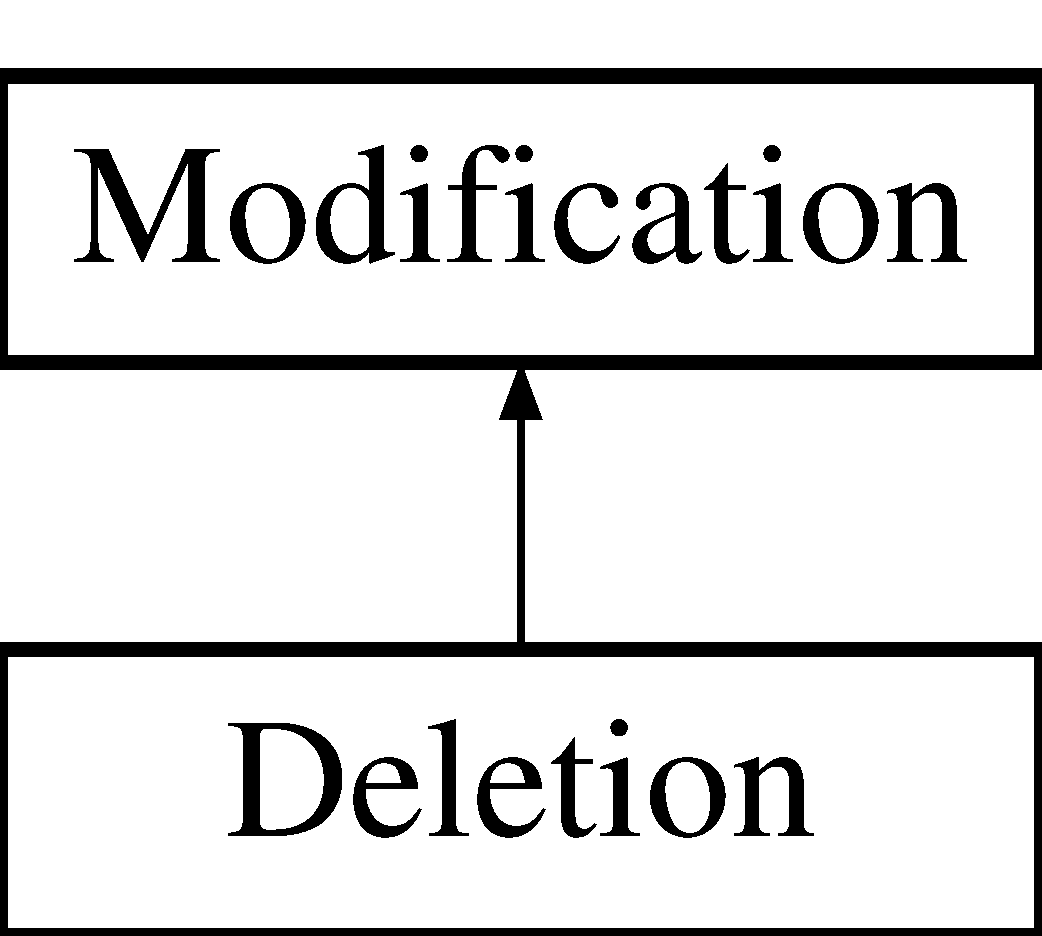
\includegraphics[height=2.000000cm]{classDeletion}
\end{center}
\end{figure}
\subsection*{Public Member Functions}
\begin{DoxyCompactItemize}
\item 
\mbox{\Hypertarget{classDeletion_a8446318e3f7004ef557b6021350fa389}\label{classDeletion_a8446318e3f7004ef557b6021350fa389}} 
{\bfseries Deletion} (\mbox{\hyperlink{classTreeObject}{Tree\+Object}} $\ast$obj, \mbox{\hyperlink{classTreeObject}{Tree\+Object}} $\ast$parent)
\item 
\mbox{\Hypertarget{classDeletion_ac5bdb21c4a8dbc8afea9910435e509a8}\label{classDeletion_ac5bdb21c4a8dbc8afea9910435e509a8}} 
void {\bfseries write\+\_\+out} (\mbox{\hyperlink{classPartitionManager}{Partition\+Manager}} $\ast$pm)
\end{DoxyCompactItemize}
\subsection*{Additional Inherited Members}


The documentation for this class was generated from the following files\+:\begin{DoxyCompactItemize}
\item 
Filesystem/\+Backend/Trees.\+h\item 
Filesystem/\+Backend/Trees.\+cpp\end{DoxyCompactItemize}

\hypertarget{classDisk}{}\section{Disk Class Reference}
\label{classDisk}\index{Disk@{Disk}}
\subsection*{Public Member Functions}
\begin{DoxyCompactItemize}
\item 
\mbox{\hyperlink{classDisk_a5be49d1002da046d1890df1b088900e4}{Disk}} (Blk\+Num\+Type numblocks, size\+\_\+t block\+Size, char $\ast$location)
\end{DoxyCompactItemize}
\begin{Indent}\textbf{ Modifier Functions}\par
\begin{DoxyCompactItemize}
\item 
void \mbox{\hyperlink{classDisk_a5d335138f56e6b87c8ebc4b6473183e7}{write\+Disk\+Block}} (Blk\+Num\+Type blknum, char $\ast$blkdata)
\end{DoxyCompactItemize}
\end{Indent}
\begin{Indent}\textbf{ Accessor Functions}\par
\begin{DoxyCompactItemize}
\item 
void \mbox{\hyperlink{classDisk_a2598cdd9013bdbb1213afa878c567daa}{read\+Disk\+Block}} (Blk\+Num\+Type blknum, char $\ast$blkdata)
\item 
size\+\_\+t \mbox{\hyperlink{classDisk_a1c149b57524fe4e7ae7c8643309e0501}{get\+Block\+Size}} ()
\item 
int \mbox{\hyperlink{classDisk_a3c61119ce5707dd4ab039201590a7c22}{get\+Block\+Count}} ()
\end{DoxyCompactItemize}
\end{Indent}


\subsection{Constructor \& Destructor Documentation}
\mbox{\Hypertarget{classDisk_a5be49d1002da046d1890df1b088900e4}\label{classDisk_a5be49d1002da046d1890df1b088900e4}} 
\index{Disk@{Disk}!Disk@{Disk}}
\index{Disk@{Disk}!Disk@{Disk}}
\subsubsection{\texorpdfstring{Disk()}{Disk()}}
{\footnotesize\ttfamily Disk\+::\+Disk (\begin{DoxyParamCaption}\item[{Blk\+Num\+Type}]{numblocks,  }\item[{size\+\_\+t}]{block\+Size,  }\item[{char $\ast$}]{location }\end{DoxyParamCaption})}


\begin{DoxyParams}{Parameters}
{\em numblocks} & the number of blocks on the \mbox{\hyperlink{classDisk}{Disk}} \\
\hline
{\em blocksize} & the block size for \mbox{\hyperlink{classDisk}{Disk}} blocks \\
\hline
{\em location} & the location of the \mbox{\hyperlink{classDisk}{Disk}} \\
\hline
\end{DoxyParams}


\subsection{Member Function Documentation}
\mbox{\Hypertarget{classDisk_a3c61119ce5707dd4ab039201590a7c22}\label{classDisk_a3c61119ce5707dd4ab039201590a7c22}} 
\index{Disk@{Disk}!get\+Block\+Count@{get\+Block\+Count}}
\index{get\+Block\+Count@{get\+Block\+Count}!Disk@{Disk}}
\subsubsection{\texorpdfstring{get\+Block\+Count()}{getBlockCount()}}
{\footnotesize\ttfamily int Disk\+::get\+Block\+Count (\begin{DoxyParamCaption}{ }\end{DoxyParamCaption})}

\begin{DoxyReturn}{Returns}
the number of blocks on the entire \mbox{\hyperlink{classDisk}{Disk}} 
\end{DoxyReturn}
\mbox{\Hypertarget{classDisk_a1c149b57524fe4e7ae7c8643309e0501}\label{classDisk_a1c149b57524fe4e7ae7c8643309e0501}} 
\index{Disk@{Disk}!get\+Block\+Size@{get\+Block\+Size}}
\index{get\+Block\+Size@{get\+Block\+Size}!Disk@{Disk}}
\subsubsection{\texorpdfstring{get\+Block\+Size()}{getBlockSize()}}
{\footnotesize\ttfamily size\+\_\+t Disk\+::get\+Block\+Size (\begin{DoxyParamCaption}{ }\end{DoxyParamCaption})}

\begin{DoxyReturn}{Returns}
the blocksize of the \mbox{\hyperlink{classDisk}{Disk}} 
\end{DoxyReturn}
\mbox{\Hypertarget{classDisk_a2598cdd9013bdbb1213afa878c567daa}\label{classDisk_a2598cdd9013bdbb1213afa878c567daa}} 
\index{Disk@{Disk}!read\+Disk\+Block@{read\+Disk\+Block}}
\index{read\+Disk\+Block@{read\+Disk\+Block}!Disk@{Disk}}
\subsubsection{\texorpdfstring{read\+Disk\+Block()}{readDiskBlock()}}
{\footnotesize\ttfamily void Disk\+::read\+Disk\+Block (\begin{DoxyParamCaption}\item[{Blk\+Num\+Type}]{blknum,  }\item[{char $\ast$}]{blkdata }\end{DoxyParamCaption})}

Reads a block from the \mbox{\hyperlink{classDisk}{Disk}}. 
\begin{DoxyParams}{Parameters}
{\em blknum} & the blocknumber to be read \\
\hline
{\em blkdata} & the buffer to put the read data. must be large enough to contain an entire block of data \\
\hline
\end{DoxyParams}
\begin{DoxySeeAlso}{See also}
Partition\+Manger\+::read\+Disk\+Block() Parition\+Manager\+::read\+Disk\+Block() 
\end{DoxySeeAlso}
\mbox{\Hypertarget{classDisk_a5d335138f56e6b87c8ebc4b6473183e7}\label{classDisk_a5d335138f56e6b87c8ebc4b6473183e7}} 
\index{Disk@{Disk}!write\+Disk\+Block@{write\+Disk\+Block}}
\index{write\+Disk\+Block@{write\+Disk\+Block}!Disk@{Disk}}
\subsubsection{\texorpdfstring{write\+Disk\+Block()}{writeDiskBlock()}}
{\footnotesize\ttfamily void Disk\+::write\+Disk\+Block (\begin{DoxyParamCaption}\item[{Blk\+Num\+Type}]{blknum,  }\item[{char $\ast$}]{blkdata }\end{DoxyParamCaption})}

Writes a block to the \mbox{\hyperlink{classDisk}{Disk}}. 
\begin{DoxyParams}{Parameters}
{\em blknum} & the blocknumber to be written \\
\hline
{\em blkdata} & the buffer to write the data from. It Will write an entire block size of data. \\
\hline
\end{DoxyParams}
\begin{DoxySeeAlso}{See also}
Partition\+Manger\+::write\+Disk\+Block() Parition\+Manager\+::write\+Disk\+Block() 
\end{DoxySeeAlso}


The documentation for this class was generated from the following files\+:\begin{DoxyCompactItemize}
\item 
Filesystem/\+Daemon\+Dependancies/\+Disk/Disk.\+h\item 
Filesystem/\+Daemon\+Dependancies/\+Disk/Disk.\+cpp\end{DoxyCompactItemize}

\hypertarget{classdisk__error}{}\section{disk\+\_\+error Class Reference}
\label{classdisk__error}\index{disk\+\_\+error@{disk\+\_\+error}}
Inheritance diagram for disk\+\_\+error\+:\begin{figure}[H]
\begin{center}
\leavevmode
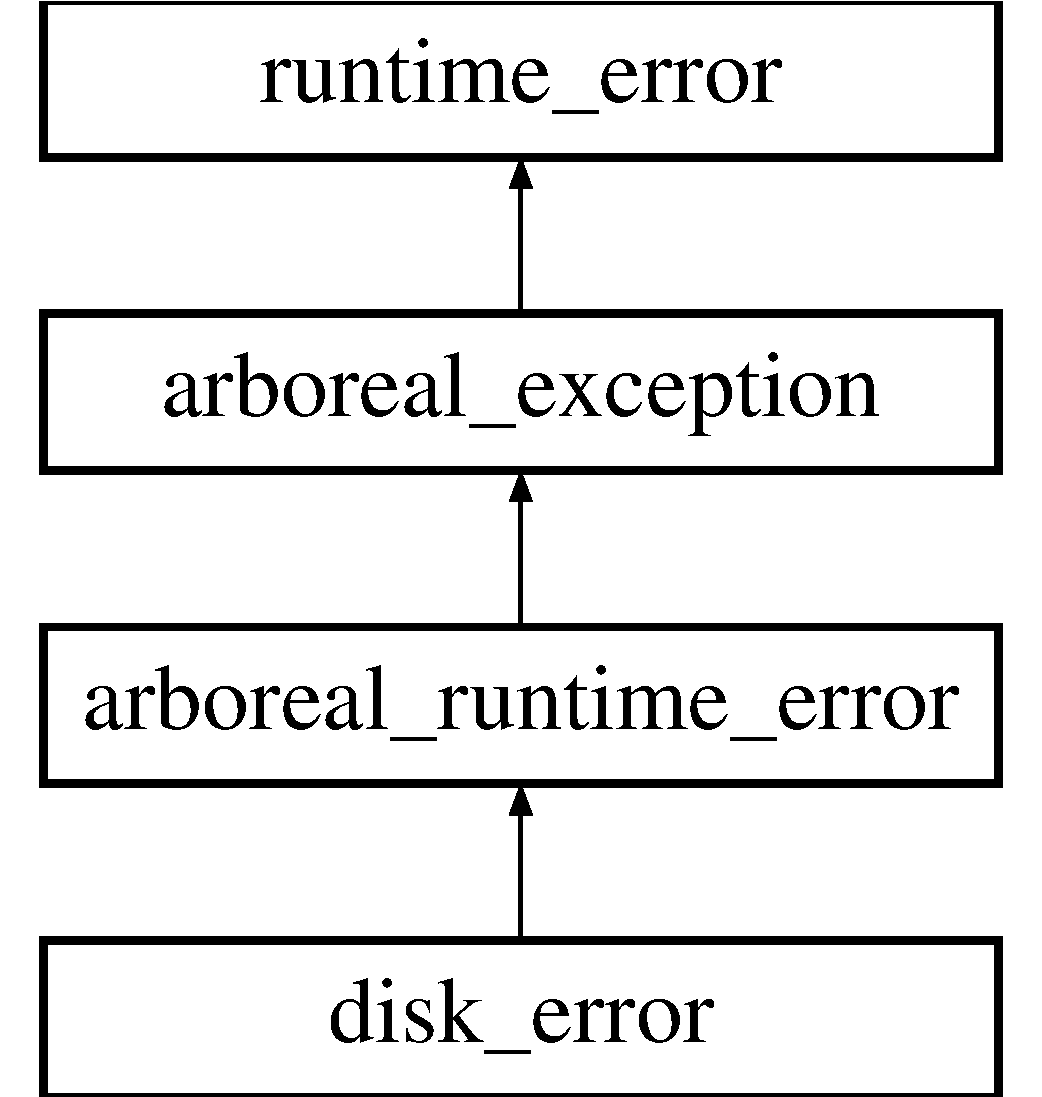
\includegraphics[height=4.000000cm]{classdisk__error}
\end{center}
\end{figure}
\subsection*{Public Member Functions}
\begin{DoxyCompactItemize}
\item 
\mbox{\Hypertarget{classdisk__error_a1f3a9f8326a8d192d3a54e698d09d29d}\label{classdisk__error_a1f3a9f8326a8d192d3a54e698d09d29d}} 
{\bfseries disk\+\_\+error} (const char $\ast$what, const char $\ast$where)
\item 
\mbox{\Hypertarget{classdisk__error_a03937aabd05ba77b2e49fff4c039b047}\label{classdisk__error_a03937aabd05ba77b2e49fff4c039b047}} 
{\bfseries disk\+\_\+error} (const char $\ast$what, const string \&where)
\item 
\mbox{\Hypertarget{classdisk__error_afb8e69ac35d47d5ed1bcc8b764baea4b}\label{classdisk__error_afb8e69ac35d47d5ed1bcc8b764baea4b}} 
{\bfseries disk\+\_\+error} (const string \&what, const string \&where)
\item 
\mbox{\Hypertarget{classdisk__error_aea5a9df17b57607f55f82de0cd384052}\label{classdisk__error_aea5a9df17b57607f55f82de0cd384052}} 
{\bfseries disk\+\_\+error} (const string \&what, const char $\ast$where)
\end{DoxyCompactItemize}
\subsection*{Additional Inherited Members}


The documentation for this class was generated from the following files\+:\begin{DoxyCompactItemize}
\item 
Filesystem/Arboreal\+\_\+\+Exceptions.\+h\item 
Filesystem/Arboreal\+\_\+\+Exceptions.\+cpp\end{DoxyCompactItemize}

\hypertarget{classDiskManager}{}\section{Disk\+Manager Class Reference}
\label{classDiskManager}\index{Disk\+Manager@{Disk\+Manager}}
\subsection*{Public Member Functions}
\begin{DoxyCompactItemize}
\item 
\mbox{\hyperlink{classDiskManager_a948cecec230d9895bafaced5534fd6cf}{Disk\+Manager}} (\mbox{\hyperlink{classDisk}{Disk}} $\ast$d)
\end{DoxyCompactItemize}
\begin{Indent}\textbf{ Accessor Functions}\par
\begin{DoxyCompactItemize}
\item 
void \mbox{\hyperlink{classDiskManager_afda24be04fb85711236a4d5905a5ad1c}{read\+Disk\+Block}} (string partition\+Name, Blk\+Num\+Type blknum, char $\ast$blkdata)
\item 
size\+\_\+t \mbox{\hyperlink{classDiskManager_aabdfbb2171f3c19a3ae14f9532876404}{get\+Block\+Size}} ()
\item 
Blk\+Num\+Type \mbox{\hyperlink{classDiskManager_ae32627ccfa72013e35da637570e1729b}{get\+Partition\+Size}} (string partition\+Name)
\item 
\mbox{\hyperlink{structDiskPartition}{Disk\+Partition}} $\ast$ \mbox{\hyperlink{classDiskManager_a08375c254bc09c8351a4f96cb669f1ab}{find\+Part}} (string partition\+Name)
\end{DoxyCompactItemize}
\end{Indent}
\begin{Indent}\textbf{ Modifier Functions}\par
\begin{DoxyCompactItemize}
\item 
void \mbox{\hyperlink{classDiskManager_ac96846d309a59e8ac7b100724329cb30}{write\+Disk\+Block}} (string partition\+Name, Blk\+Num\+Type blknum, char $\ast$blkdata)
\end{DoxyCompactItemize}
\end{Indent}


\subsection{Constructor \& Destructor Documentation}
\mbox{\Hypertarget{classDiskManager_a948cecec230d9895bafaced5534fd6cf}\label{classDiskManager_a948cecec230d9895bafaced5534fd6cf}} 
\index{Disk\+Manager@{Disk\+Manager}!Disk\+Manager@{Disk\+Manager}}
\index{Disk\+Manager@{Disk\+Manager}!Disk\+Manager@{Disk\+Manager}}
\subsubsection{\texorpdfstring{Disk\+Manager()}{DiskManager()}}
{\footnotesize\ttfamily Disk\+Manager\+::\+Disk\+Manager (\begin{DoxyParamCaption}\item[{\mbox{\hyperlink{classDisk}{Disk}} $\ast$}]{d }\end{DoxyParamCaption})}


\begin{DoxyParams}{Parameters}
{\em d} & Pointer to the \mbox{\hyperlink{classDisk}{Disk}} this will manage \\
\hline
\end{DoxyParams}


\subsection{Member Function Documentation}
\mbox{\Hypertarget{classDiskManager_a08375c254bc09c8351a4f96cb669f1ab}\label{classDiskManager_a08375c254bc09c8351a4f96cb669f1ab}} 
\index{Disk\+Manager@{Disk\+Manager}!find\+Part@{find\+Part}}
\index{find\+Part@{find\+Part}!Disk\+Manager@{Disk\+Manager}}
\subsubsection{\texorpdfstring{find\+Part()}{findPart()}}
{\footnotesize\ttfamily \mbox{\hyperlink{structDiskPartition}{Disk\+Partition}} $\ast$ Disk\+Manager\+::find\+Part (\begin{DoxyParamCaption}\item[{string}]{partition\+Name }\end{DoxyParamCaption})}


\begin{DoxyParams}{Parameters}
{\em partition\+Name} & the name of the partition \\
\hline
\end{DoxyParams}
\begin{DoxyReturn}{Returns}
the size of a partition in blocks 
\end{DoxyReturn}
\mbox{\Hypertarget{classDiskManager_aabdfbb2171f3c19a3ae14f9532876404}\label{classDiskManager_aabdfbb2171f3c19a3ae14f9532876404}} 
\index{Disk\+Manager@{Disk\+Manager}!get\+Block\+Size@{get\+Block\+Size}}
\index{get\+Block\+Size@{get\+Block\+Size}!Disk\+Manager@{Disk\+Manager}}
\subsubsection{\texorpdfstring{get\+Block\+Size()}{getBlockSize()}}
{\footnotesize\ttfamily size\+\_\+t Disk\+Manager\+::get\+Block\+Size (\begin{DoxyParamCaption}{ }\end{DoxyParamCaption})}

\begin{DoxyReturn}{Returns}
the blocksize of the \mbox{\hyperlink{classDisk}{Disk}} 
\end{DoxyReturn}
\mbox{\Hypertarget{classDiskManager_ae32627ccfa72013e35da637570e1729b}\label{classDiskManager_ae32627ccfa72013e35da637570e1729b}} 
\index{Disk\+Manager@{Disk\+Manager}!get\+Partition\+Size@{get\+Partition\+Size}}
\index{get\+Partition\+Size@{get\+Partition\+Size}!Disk\+Manager@{Disk\+Manager}}
\subsubsection{\texorpdfstring{get\+Partition\+Size()}{getPartitionSize()}}
{\footnotesize\ttfamily Blk\+Num\+Type Disk\+Manager\+::get\+Partition\+Size (\begin{DoxyParamCaption}\item[{string}]{partition\+Name }\end{DoxyParamCaption})}


\begin{DoxyParams}{Parameters}
{\em partition\+Name} & the name of the partition \\
\hline
\end{DoxyParams}
\begin{DoxyReturn}{Returns}
the size of a partition in blocks 
\end{DoxyReturn}
\mbox{\Hypertarget{classDiskManager_afda24be04fb85711236a4d5905a5ad1c}\label{classDiskManager_afda24be04fb85711236a4d5905a5ad1c}} 
\index{Disk\+Manager@{Disk\+Manager}!read\+Disk\+Block@{read\+Disk\+Block}}
\index{read\+Disk\+Block@{read\+Disk\+Block}!Disk\+Manager@{Disk\+Manager}}
\subsubsection{\texorpdfstring{read\+Disk\+Block()}{readDiskBlock()}}
{\footnotesize\ttfamily void Disk\+Manager\+::read\+Disk\+Block (\begin{DoxyParamCaption}\item[{string}]{partition\+Name,  }\item[{Blk\+Num\+Type}]{blknum,  }\item[{char $\ast$}]{blkdata }\end{DoxyParamCaption})}

Reads a block from the \mbox{\hyperlink{classDisk}{Disk}}. 
\begin{DoxyParams}{Parameters}
{\em partition\+Name} & the name of the partition to write the block to \\
\hline
{\em blknum} & the blocknumber to be read \\
\hline
{\em blkdata} & the buffer to put the read data. must be large enough to contain an entire block of data \\
\hline
\end{DoxyParams}
\begin{DoxySeeAlso}{See also}
Partition\+Manger\+::read\+Disk\+Block() Parition\+Manager\+::read\+Disk\+Block() 
\end{DoxySeeAlso}
\mbox{\Hypertarget{classDiskManager_ac96846d309a59e8ac7b100724329cb30}\label{classDiskManager_ac96846d309a59e8ac7b100724329cb30}} 
\index{Disk\+Manager@{Disk\+Manager}!write\+Disk\+Block@{write\+Disk\+Block}}
\index{write\+Disk\+Block@{write\+Disk\+Block}!Disk\+Manager@{Disk\+Manager}}
\subsubsection{\texorpdfstring{write\+Disk\+Block()}{writeDiskBlock()}}
{\footnotesize\ttfamily void Disk\+Manager\+::write\+Disk\+Block (\begin{DoxyParamCaption}\item[{string}]{partition\+Name,  }\item[{Blk\+Num\+Type}]{blknum,  }\item[{char $\ast$}]{blkdata }\end{DoxyParamCaption})}

Writes a block to the \mbox{\hyperlink{classDisk}{Disk}}. 
\begin{DoxyParams}{Parameters}
{\em partition\+Name} & the name of the partition to write the block to \\
\hline
{\em blknum} & the blocknumber to be written \\
\hline
{\em blkdata} & the buffer to write the data from. It Will write an entire block size of data. \\
\hline
\end{DoxyParams}
\begin{DoxySeeAlso}{See also}
Partition\+Manger\+::write\+Disk\+Block() Parition\+Manager\+::write\+Disk\+Block() 
\end{DoxySeeAlso}


The documentation for this class was generated from the following files\+:\begin{DoxyCompactItemize}
\item 
Filesystem/\+Daemon\+Dependancies/\+Disk\+Manager/Disk\+Manager.\+h\item 
Filesystem/\+Daemon\+Dependancies/\+Disk\+Manager/Disk\+Manager.\+cpp\end{DoxyCompactItemize}

\hypertarget{structDiskPartition}{}\section{Disk\+Partition Struct Reference}
\label{structDiskPartition}\index{Disk\+Partition@{Disk\+Partition}}
\subsection*{Public Attributes}
\begin{DoxyCompactItemize}
\item 
\mbox{\Hypertarget{structDiskPartition_a8c89b5f115fa534a3cb5d76505de97cb}\label{structDiskPartition_a8c89b5f115fa534a3cb5d76505de97cb}} 
string {\bfseries partition\+Name}
\item 
\mbox{\Hypertarget{structDiskPartition_a61dfe31b8baf361738168c2521c19286}\label{structDiskPartition_a61dfe31b8baf361738168c2521c19286}} 
Blk\+Num\+Type {\bfseries partition\+Size}
\item 
\mbox{\Hypertarget{structDiskPartition_a2b5b89e7739ffa6ac21772a92f88e35f}\label{structDiskPartition_a2b5b89e7739ffa6ac21772a92f88e35f}} 
Blk\+Num\+Type {\bfseries partition\+Blk\+Start}
\item 
\mbox{\Hypertarget{structDiskPartition_a6fd44394d9d8bf83fa61cfd12be25412}\label{structDiskPartition_a6fd44394d9d8bf83fa61cfd12be25412}} 
int {\bfseries file\+Name\+Size}
\end{DoxyCompactItemize}


The documentation for this struct was generated from the following file\+:\begin{DoxyCompactItemize}
\item 
Filesystem/\+Backend/Disk\+Manager.\+h\end{DoxyCompactItemize}

\hypertarget{classFile}{}\section{File Class Reference}
\label{classFile}\index{File@{File}}
\subsection*{Public Member Functions}
\begin{DoxyCompactItemize}
\item 
\mbox{\hyperlink{classFile_af29e498f601951f4ccf06f2fc3fb1f73}{File}} (string name, const vector$<$ string $>$ \&tags, \mbox{\hyperlink{structfile__attributes}{File\+Attributes}} attributes)
\end{DoxyCompactItemize}
\begin{Indent}\textbf{ Accessor Functions}\par
\begin{DoxyCompactItemize}
\item 
string \mbox{\hyperlink{classFile_a4b8e86f4fae0219744cf82f6bab35b53}{get\+\_\+name}} ()
\item 
vector$<$ string $>$ \& \mbox{\hyperlink{classFile_a479270bfe1fa436d317151ac108eb28a}{get\+\_\+tags}} ()
\item 
\mbox{\hyperlink{structfile__attributes}{File\+Attributes}} \mbox{\hyperlink{classFile_a9f59d3d546e8e574889558d63c71bf02}{get\+\_\+attributes}} ()
\end{DoxyCompactItemize}
\end{Indent}
\subsection*{Static Public Member Functions}
\begin{DoxyCompactItemize}
\item 
static \mbox{\hyperlink{classFile}{File}} $\ast$ \mbox{\hyperlink{classFile_a1118d477e6b00d789e948e8cca5ae393}{read\+\_\+buff}} (const char $\ast$serialized\+File)
\end{DoxyCompactItemize}


\subsection{Constructor \& Destructor Documentation}
\mbox{\Hypertarget{classFile_af29e498f601951f4ccf06f2fc3fb1f73}\label{classFile_af29e498f601951f4ccf06f2fc3fb1f73}} 
\index{File@{File}!File@{File}}
\index{File@{File}!File@{File}}
\subsubsection{\texorpdfstring{File()}{File()}}
{\footnotesize\ttfamily File\+::\+File (\begin{DoxyParamCaption}\item[{string}]{name,  }\item[{const vector$<$ string $>$ \&}]{tags,  }\item[{\mbox{\hyperlink{structfile__attributes}{File\+Attributes}}}]{attributes }\end{DoxyParamCaption})}


\begin{DoxyParams}{Parameters}
{\em name} & the name of the \mbox{\hyperlink{classFile}{File}} \\
\hline
{\em tags} & the tags to be associated with the \mbox{\hyperlink{classFile}{File}} \\
\hline
{\em attributes} & the \mbox{\hyperlink{classFile}{File}} attributes \\
\hline
\end{DoxyParams}


\subsection{Member Function Documentation}
\mbox{\Hypertarget{classFile_a9f59d3d546e8e574889558d63c71bf02}\label{classFile_a9f59d3d546e8e574889558d63c71bf02}} 
\index{File@{File}!get\+\_\+attributes@{get\+\_\+attributes}}
\index{get\+\_\+attributes@{get\+\_\+attributes}!File@{File}}
\subsubsection{\texorpdfstring{get\+\_\+attributes()}{get\_attributes()}}
{\footnotesize\ttfamily \mbox{\hyperlink{structfile__attributes}{File\+Attributes}} File\+::get\+\_\+attributes (\begin{DoxyParamCaption}{ }\end{DoxyParamCaption})}

\begin{DoxyReturn}{Returns}
the attributes associated with this \mbox{\hyperlink{classFile}{File}} 
\end{DoxyReturn}
\mbox{\Hypertarget{classFile_a4b8e86f4fae0219744cf82f6bab35b53}\label{classFile_a4b8e86f4fae0219744cf82f6bab35b53}} 
\index{File@{File}!get\+\_\+name@{get\+\_\+name}}
\index{get\+\_\+name@{get\+\_\+name}!File@{File}}
\subsubsection{\texorpdfstring{get\+\_\+name()}{get\_name()}}
{\footnotesize\ttfamily string File\+::get\+\_\+name (\begin{DoxyParamCaption}{ }\end{DoxyParamCaption})}

\begin{DoxyReturn}{Returns}
The name of the \mbox{\hyperlink{classFile}{File}} 
\end{DoxyReturn}
\mbox{\Hypertarget{classFile_a479270bfe1fa436d317151ac108eb28a}\label{classFile_a479270bfe1fa436d317151ac108eb28a}} 
\index{File@{File}!get\+\_\+tags@{get\+\_\+tags}}
\index{get\+\_\+tags@{get\+\_\+tags}!File@{File}}
\subsubsection{\texorpdfstring{get\+\_\+tags()}{get\_tags()}}
{\footnotesize\ttfamily vector$<$ string $>$ \& File\+::get\+\_\+tags (\begin{DoxyParamCaption}{ }\end{DoxyParamCaption})}

\begin{DoxyReturn}{Returns}
The tags associated with this \mbox{\hyperlink{classFile}{File}} 
\end{DoxyReturn}
\mbox{\Hypertarget{classFile_a1118d477e6b00d789e948e8cca5ae393}\label{classFile_a1118d477e6b00d789e948e8cca5ae393}} 
\index{File@{File}!read\+\_\+buff@{read\+\_\+buff}}
\index{read\+\_\+buff@{read\+\_\+buff}!File@{File}}
\subsubsection{\texorpdfstring{read\+\_\+buff()}{read\_buff()}}
{\footnotesize\ttfamily \mbox{\hyperlink{classFile}{File}} $\ast$ File\+::read\+\_\+buff (\begin{DoxyParamCaption}\item[{const char $\ast$}]{serialized\+File }\end{DoxyParamCaption})\hspace{0.3cm}{\ttfamily [static]}}

Will take a char$\ast$ buffer and create a \mbox{\hyperlink{classFile}{File}} object from it. The buffer must have been serialized in the correct format 
\begin{DoxyParams}{Parameters}
{\em serialized\+File} & the serialized\+File object \\
\hline
\end{DoxyParams}
\begin{DoxyReturn}{Returns}
a File$\ast$ to the created \mbox{\hyperlink{classFile}{File}} 
\end{DoxyReturn}
\begin{DoxySeeAlso}{See also}
\mbox{\hyperlink{classFileInfo_a64fc62c3e376dfd61088932d8b793589}{File\+Info\+::serialize()}} 
\end{DoxySeeAlso}


The documentation for this class was generated from the following files\+:\begin{DoxyCompactItemize}
\item 
Filesystem/File.\+h\item 
Filesystem/File.\+cpp\end{DoxyCompactItemize}

\hypertarget{structfile__attributes}{}\section{file\+\_\+attributes Struct Reference}
\label{structfile__attributes}\index{file\+\_\+attributes@{file\+\_\+attributes}}
\subsection*{Public Attributes}
\begin{DoxyCompactItemize}
\item 
\mbox{\Hypertarget{structfile__attributes_a9fa92e6a7d6ac7f18df7940697524411}\label{structfile__attributes_a9fa92e6a7d6ac7f18df7940697524411}} 
time\+\_\+t {\bfseries creation\+Time}
\item 
\mbox{\Hypertarget{structfile__attributes_a9b16144fd6ce8d982afc738058f07fa3}\label{structfile__attributes_a9b16144fd6ce8d982afc738058f07fa3}} 
time\+\_\+t {\bfseries last\+Access}
\item 
\mbox{\Hypertarget{structfile__attributes_ad4592775c8cb9a899a12ca551329a936}\label{structfile__attributes_ad4592775c8cb9a899a12ca551329a936}} 
time\+\_\+t {\bfseries last\+Edit}
\item 
\mbox{\Hypertarget{structfile__attributes_a753691702c194d2e43c0fb62e6cd4ee1}\label{structfile__attributes_a753691702c194d2e43c0fb62e6cd4ee1}} 
size\+\_\+t {\bfseries size}
\item 
\mbox{\Hypertarget{structfile__attributes_a6af710c43bfc31b1a005c9ad7251f801}\label{structfile__attributes_a6af710c43bfc31b1a005c9ad7251f801}} 
char {\bfseries permissions} \mbox{[}12\mbox{]}
\item 
\mbox{\Hypertarget{structfile__attributes_a74be4a864fa3f38eff632b4b25654b97}\label{structfile__attributes_a74be4a864fa3f38eff632b4b25654b97}} 
int {\bfseries owner}
\end{DoxyCompactItemize}


The documentation for this struct was generated from the following file\+:\begin{DoxyCompactItemize}
\item 
types.\+h\end{DoxyCompactItemize}

\hypertarget{classfile__error}{}\section{file\+\_\+error Class Reference}
\label{classfile__error}\index{file\+\_\+error@{file\+\_\+error}}
Inheritance diagram for file\+\_\+error\+:\begin{figure}[H]
\begin{center}
\leavevmode
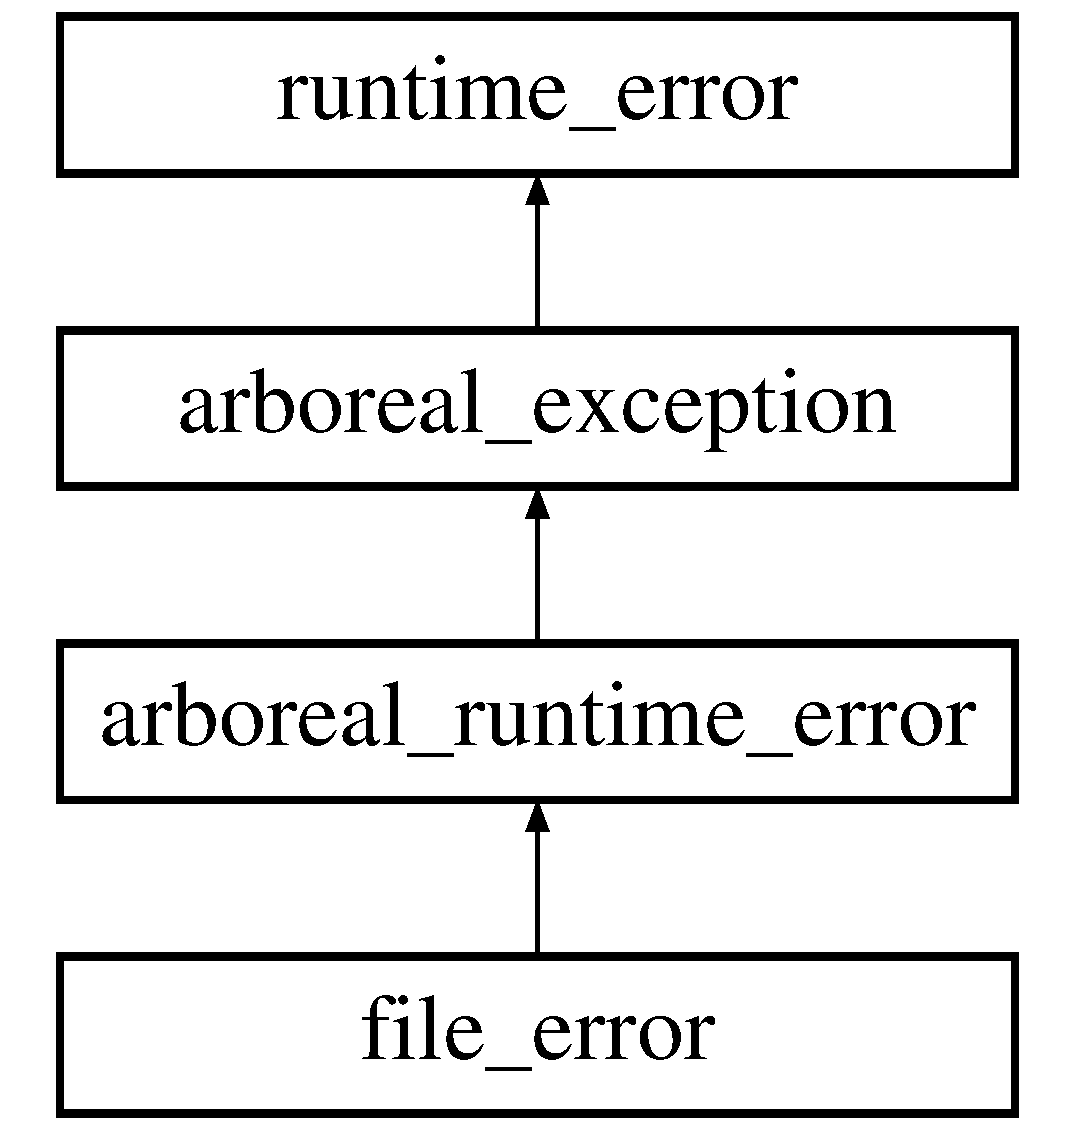
\includegraphics[height=4.000000cm]{db/ddf/classfile__error}
\end{center}
\end{figure}
\subsection*{Public Member Functions}
\begin{DoxyCompactItemize}
\item 
\mbox{\Hypertarget{classfile__error_a10da41c5d15b25fdafa97ae79523e242}\label{classfile__error_a10da41c5d15b25fdafa97ae79523e242}} 
{\bfseries file\+\_\+error} (const char $\ast$what, const char $\ast$where, const int ecode=99)
\item 
\mbox{\Hypertarget{classfile__error_ae70ca16a0a8eee95a88a64128b7fcbad}\label{classfile__error_ae70ca16a0a8eee95a88a64128b7fcbad}} 
{\bfseries file\+\_\+error} (const char $\ast$what, const string \&where, const int ecode=99)
\item 
\mbox{\Hypertarget{classfile__error_a9b1c03f989df972ca3201f984ddece6d}\label{classfile__error_a9b1c03f989df972ca3201f984ddece6d}} 
{\bfseries file\+\_\+error} (const string \&what, const string \&where, const int ecode=99)
\item 
\mbox{\Hypertarget{classfile__error_a2698ca75c20dd3ffc5adb8d470fff246}\label{classfile__error_a2698ca75c20dd3ffc5adb8d470fff246}} 
{\bfseries file\+\_\+error} (const string \&what, const char $\ast$where, const int ecode=99)
\end{DoxyCompactItemize}
\subsection*{Additional Inherited Members}


The documentation for this class was generated from the following files\+:\begin{DoxyCompactItemize}
\item 
Shared\+Headers/Arboreal\+\_\+\+Exceptions.\+h\item 
Shared\+C\+P\+P\+Files/Arboreal\+\_\+\+Exceptions.\+cpp\end{DoxyCompactItemize}

\hypertarget{classFileInfo}{}\section{File\+Info Class Reference}
\label{classFileInfo}\index{File\+Info@{File\+Info}}
Inheritance diagram for File\+Info\+:\begin{figure}[H]
\begin{center}
\leavevmode
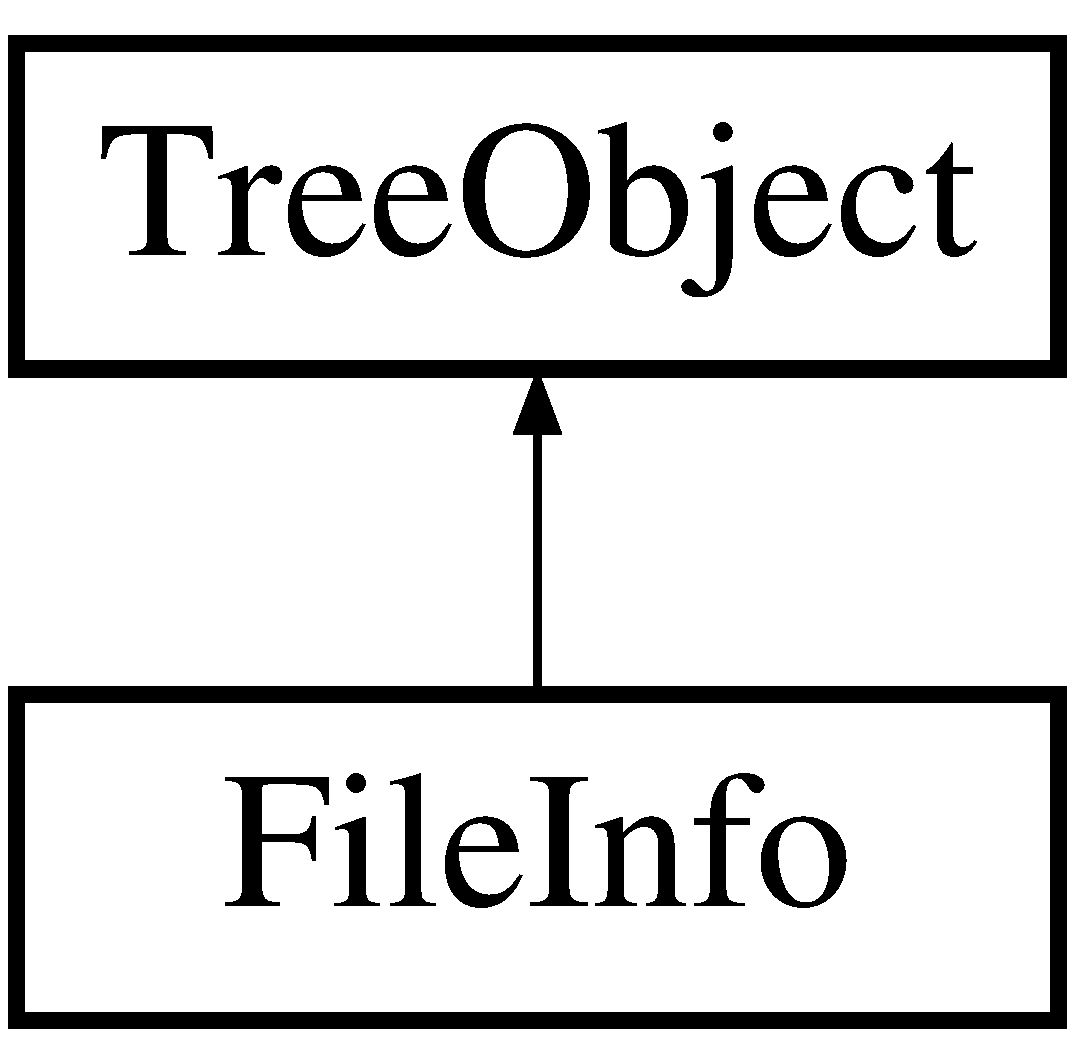
\includegraphics[height=2.000000cm]{classFileInfo}
\end{center}
\end{figure}
\subsection*{Public Member Functions}
\begin{DoxyCompactItemize}
\item 
\mbox{\hyperlink{classFileInfo_a3586bb4f50c4a0f63ff4ea0a1e56ce9c}{File\+Info}} (string filename, Blk\+Num\+Type blknum, \mbox{\hyperlink{classPartitionManager}{Partition\+Manager}} $\ast$pm)
\item 
void \mbox{\hyperlink{classFileInfo_a8e835f000ddfd0f1097ccfa7e7801a09}{write\+\_\+out}} ()
\item 
void \mbox{\hyperlink{classFileInfo_a2bf60d4be97347f3d7a15cf839afca7d}{read\+\_\+in}} (unordered\+\_\+multimap$<$ string, \mbox{\hyperlink{classFileInfo}{File\+Info}} $\ast$$>$ $\ast$all\+Files, \mbox{\hyperlink{classRootTree}{Root\+Tree}} $\ast$root\+Tree)
\item 
void \mbox{\hyperlink{classFileInfo_ae058242283d3317eaf2b79428e6137f6}{erase}} (string name)
\item 
void \mbox{\hyperlink{classFileInfo_ad93a84b63e417b07aa68b619051ab746}{insert}} (string name, \mbox{\hyperlink{classTreeObject}{Tree\+Object}} $\ast$ptr)
\item 
void \mbox{\hyperlink{classFileInfo_a2ca34d945ed1208f227a249ba72ee427}{del}} ()
\item 
void \mbox{\hyperlink{classFileInfo_a8c6b58cb9f7e9978064291ef81380e01}{delete\+\_\+cont\+\_\+blocks}} (Blk\+Num\+Type blknum)
\item 
void \mbox{\hyperlink{classFileInfo_a7f788f31521c535646eebfa9959bbb24}{insert\+\_\+addition}} (\mbox{\hyperlink{classTreeObject}{Tree\+Object}} $\ast$add)
\item 
void \mbox{\hyperlink{classFileInfo_a278136b1d68f55dc56a4be807076fc0d}{insert\+\_\+deletion}} (\mbox{\hyperlink{classTreeObject}{Tree\+Object}} $\ast$\mbox{\hyperlink{classFileInfo_a2ca34d945ed1208f227a249ba72ee427}{del}})
\end{DoxyCompactItemize}
\begin{Indent}\textbf{ Accessor Functions}\par
\begin{DoxyCompactItemize}
\item 
string \mbox{\hyperlink{classFileInfo_a96827c2e48fb1a15d468e9afd545383e}{mangle}} ()
\begin{DoxyCompactList}\small\item\em mangles the filename with its tags \end{DoxyCompactList}\item 
string \mbox{\hyperlink{classFileInfo_a105ad751f21bead6fc2a76e79cb3b701}{mangle}} (vector$<$ string $>$ \&tags)
\begin{DoxyCompactList}\small\item\em mangles the filename with the specified tags \end{DoxyCompactList}\item 
string \mbox{\hyperlink{classFileInfo_aec8a60addbed54097f6cac0a6a516717}{mangle}} (unordered\+\_\+set$<$ string $>$ \&tags)
\begin{DoxyCompactList}\small\item\em mangles the filename with the specified tags \end{DoxyCompactList}\item 
\mbox{\hyperlink{structfinode}{Finode}} \mbox{\hyperlink{classFileInfo_a706117270bcf31739d7ce0aa0d79891f}{get\+\_\+finode}} ()
\item 
size\+\_\+t \mbox{\hyperlink{classFileInfo_aa07a5b95bfd41814b7fb2ee30a279c65}{get\+\_\+file\+\_\+size}} ()
\item 
\mbox{\hyperlink{classAttributes}{Attributes}} $\ast$ \mbox{\hyperlink{classFileInfo_a07f09582ef3c3beb105906d5c71234a5}{get\+\_\+attributes}} ()
\item 
\mbox{\Hypertarget{classFileInfo_a0acbb8eead54541137757001474fa689}\label{classFileInfo_a0acbb8eead54541137757001474fa689}} 
\mbox{\hyperlink{structfile__attributes}{File\+Attributes}} {\bfseries get\+\_\+file\+\_\+attributes} ()
\item 
unordered\+\_\+set$<$ string $>$ \mbox{\hyperlink{classFileInfo_a63d01334c1c2ae22e5d1930afa5c74d4}{get\+\_\+tags}} ()
\item 
\mbox{\Hypertarget{classFileInfo_ad66648be9d256ac110cdcf204a3eacc7}\label{classFileInfo_ad66648be9d256ac110cdcf204a3eacc7}} 
vector$<$ string $>$ {\bfseries get\+\_\+vec\+\_\+tags} ()
\end{DoxyCompactItemize}
\end{Indent}
\begin{Indent}\textbf{ Modifier Functions}\par
\begin{DoxyCompactItemize}
\item 
void \mbox{\hyperlink{classFileInfo_a1537d2ac2b5c170d144911c8337c81bc}{add\+\_\+direct\+\_\+block}} (Blk\+Num\+Type blknum, int \mbox{\hyperlink{structindex}{index}})
\item 
void \mbox{\hyperlink{classFileInfo_a074956f43b5a6900205a541dbeaeb8c5}{add\+\_\+indirect\+\_\+block}} (Blk\+Num\+Type blknum, short level)
\item 
void \mbox{\hyperlink{classFileInfo_a3c548a8dfcb6530bfef7551ac24ca473}{update\+\_\+file\+\_\+size}} (size\+\_\+t bytes)
\item 
void \mbox{\hyperlink{classFileInfo_aacaeadeeb41726f8cbea0b7cb1ff6a22}{set\+\_\+access}} ()
\item 
void \mbox{\hyperlink{classFileInfo_a05eb10c6804660ecd47e556c27ecd019}{set\+\_\+edit}} ()
\item 
void \mbox{\hyperlink{classFileInfo_a377208012195dba0b24723837f6db39f}{set\+\_\+permissions}} (char $\ast$perms)
\begin{DoxyCompactList}\small\item\em sets the permisssions for this file \end{DoxyCompactList}\end{DoxyCompactItemize}
\end{Indent}
\subsection*{Static Public Member Functions}
\begin{DoxyCompactItemize}
\item 
static string $\ast$ \mbox{\hyperlink{classFileInfo_a64fc62c3e376dfd61088932d8b793589}{serialize}} (\mbox{\hyperlink{classFileInfo}{File\+Info}} $\ast$file)
\end{DoxyCompactItemize}
\subsection*{Additional Inherited Members}


\subsection{Constructor \& Destructor Documentation}
\mbox{\Hypertarget{classFileInfo_a3586bb4f50c4a0f63ff4ea0a1e56ce9c}\label{classFileInfo_a3586bb4f50c4a0f63ff4ea0a1e56ce9c}} 
\index{File\+Info@{File\+Info}!File\+Info@{File\+Info}}
\index{File\+Info@{File\+Info}!File\+Info@{File\+Info}}
\subsubsection{\texorpdfstring{File\+Info()}{FileInfo()}}
{\footnotesize\ttfamily File\+Info\+::\+File\+Info (\begin{DoxyParamCaption}\item[{string}]{filename,  }\item[{Blk\+Num\+Type}]{blknum,  }\item[{\mbox{\hyperlink{classPartitionManager}{Partition\+Manager}} $\ast$}]{pm }\end{DoxyParamCaption})}


\begin{DoxyParams}{Parameters}
{\em filename} & Name of the \mbox{\hyperlink{classFile}{File}} \\
\hline
{\em blknum} & the blocknumber of the associated Finode on disk \\
\hline
\end{DoxyParams}


\subsection{Member Function Documentation}
\mbox{\Hypertarget{classFileInfo_a1537d2ac2b5c170d144911c8337c81bc}\label{classFileInfo_a1537d2ac2b5c170d144911c8337c81bc}} 
\index{File\+Info@{File\+Info}!add\+\_\+direct\+\_\+block@{add\+\_\+direct\+\_\+block}}
\index{add\+\_\+direct\+\_\+block@{add\+\_\+direct\+\_\+block}!File\+Info@{File\+Info}}
\subsubsection{\texorpdfstring{add\+\_\+direct\+\_\+block()}{add\_direct\_block()}}
{\footnotesize\ttfamily void File\+Info\+::add\+\_\+direct\+\_\+block (\begin{DoxyParamCaption}\item[{Blk\+Num\+Type}]{blknum,  }\item[{int}]{index }\end{DoxyParamCaption})}

adds the specified blocknumber to the array of direct blocks in this file\textquotesingle{}s Finode 
\begin{DoxyParams}{Parameters}
{\em blknum} & the block number of the direct block that has already been allocated \\
\hline
{\em index} & the index of the blknum in the array, must be less than 12 and at least 0. \\
\hline
\end{DoxyParams}

\begin{DoxyExceptions}{Exceptions}
{\em \mbox{\hyperlink{classarboreal__logic__error}{arboreal\+\_\+logic\+\_\+error}}} & index out of bounds \\
\hline
\end{DoxyExceptions}
\begin{DoxySeeAlso}{See also}
\mbox{\hyperlink{classFileInfo_a074956f43b5a6900205a541dbeaeb8c5}{add\+\_\+indirect\+\_\+block}} 
\end{DoxySeeAlso}
\mbox{\Hypertarget{classFileInfo_a074956f43b5a6900205a541dbeaeb8c5}\label{classFileInfo_a074956f43b5a6900205a541dbeaeb8c5}} 
\index{File\+Info@{File\+Info}!add\+\_\+indirect\+\_\+block@{add\+\_\+indirect\+\_\+block}}
\index{add\+\_\+indirect\+\_\+block@{add\+\_\+indirect\+\_\+block}!File\+Info@{File\+Info}}
\subsubsection{\texorpdfstring{add\+\_\+indirect\+\_\+block()}{add\_indirect\_block()}}
{\footnotesize\ttfamily void File\+Info\+::add\+\_\+indirect\+\_\+block (\begin{DoxyParamCaption}\item[{Blk\+Num\+Type}]{blknum,  }\item[{short}]{level }\end{DoxyParamCaption})}

adds the specified blocknumber to the Finode as the start of the specified level of indirect blocks 
\begin{DoxyParams}{Parameters}
{\em blknum} & the block number of the indirect block that has already been allocated \\
\hline
{\em level} & the level that the block number is associated with. must be 1, 2 or 3. \\
\hline
\end{DoxyParams}

\begin{DoxyExceptions}{Exceptions}
{\em \mbox{\hyperlink{classarboreal__logic__error}{arboreal\+\_\+logic\+\_\+error}}} & Invalid level \\
\hline
\end{DoxyExceptions}
\begin{DoxySeeAlso}{See also}
\mbox{\hyperlink{classFileInfo_a1537d2ac2b5c170d144911c8337c81bc}{add\+\_\+direct\+\_\+block}} 
\end{DoxySeeAlso}
\mbox{\Hypertarget{classFileInfo_a2ca34d945ed1208f227a249ba72ee427}\label{classFileInfo_a2ca34d945ed1208f227a249ba72ee427}} 
\index{File\+Info@{File\+Info}!del@{del}}
\index{del@{del}!File\+Info@{File\+Info}}
\subsubsection{\texorpdfstring{del()}{del()}}
{\footnotesize\ttfamily void File\+Info\+::del (\begin{DoxyParamCaption}{ }\end{DoxyParamCaption})\hspace{0.3cm}{\ttfamily [virtual]}}

Will completely remove the \mbox{\hyperlink{classTreeObject}{Tree\+Object}}\textquotesingle{}s presence on disk 

Implements \mbox{\hyperlink{classTreeObject_af390b7479aa972888e594c07a85740b6}{Tree\+Object}}.

\mbox{\Hypertarget{classFileInfo_a8c6b58cb9f7e9978064291ef81380e01}\label{classFileInfo_a8c6b58cb9f7e9978064291ef81380e01}} 
\index{File\+Info@{File\+Info}!delete\+\_\+cont\+\_\+blocks@{delete\+\_\+cont\+\_\+blocks}}
\index{delete\+\_\+cont\+\_\+blocks@{delete\+\_\+cont\+\_\+blocks}!File\+Info@{File\+Info}}
\subsubsection{\texorpdfstring{delete\+\_\+cont\+\_\+blocks()}{delete\_cont\_blocks()}}
{\footnotesize\ttfamily void File\+Info\+::delete\+\_\+cont\+\_\+blocks (\begin{DoxyParamCaption}\item[{Blk\+Num\+Type}]{blknum }\end{DoxyParamCaption})\hspace{0.3cm}{\ttfamily [virtual]}}

Will follow the chain of continuation blocks and free all of them 
\begin{DoxyParams}{Parameters}
{\em blknum} & will free the blknum and use it to follow the chain of continuation blocks \\
\hline
\end{DoxyParams}


Reimplemented from \mbox{\hyperlink{classTreeObject_a07f5f5de1cff0cfdc2372e81559f5181}{Tree\+Object}}.

\mbox{\Hypertarget{classFileInfo_ae058242283d3317eaf2b79428e6137f6}\label{classFileInfo_ae058242283d3317eaf2b79428e6137f6}} 
\index{File\+Info@{File\+Info}!erase@{erase}}
\index{erase@{erase}!File\+Info@{File\+Info}}
\subsubsection{\texorpdfstring{erase()}{erase()}}
{\footnotesize\ttfamily void File\+Info\+::erase (\begin{DoxyParamCaption}\item[{string}]{name }\end{DoxyParamCaption})\hspace{0.3cm}{\ttfamily [virtual]}}

Disassociate the given name from this object 
\begin{DoxyParams}{Parameters}
{\em name} & the name of the object to be erased. \\
\hline
\end{DoxyParams}

\begin{DoxyExceptions}{Exceptions}
{\em \mbox{\hyperlink{classarboreal__logic__error}{arboreal\+\_\+logic\+\_\+error}}} & \\
\hline
\end{DoxyExceptions}


Reimplemented from \mbox{\hyperlink{classTreeObject_a453b5df2a9ef7c6faad259900d574ee2}{Tree\+Object}}.

\mbox{\Hypertarget{classFileInfo_a07f09582ef3c3beb105906d5c71234a5}\label{classFileInfo_a07f09582ef3c3beb105906d5c71234a5}} 
\index{File\+Info@{File\+Info}!get\+\_\+attributes@{get\+\_\+attributes}}
\index{get\+\_\+attributes@{get\+\_\+attributes}!File\+Info@{File\+Info}}
\subsubsection{\texorpdfstring{get\+\_\+attributes()}{get\_attributes()}}
{\footnotesize\ttfamily \mbox{\hyperlink{classAttributes}{Attributes}} $\ast$ File\+Info\+::get\+\_\+attributes (\begin{DoxyParamCaption}{ }\end{DoxyParamCaption})}

\begin{DoxyReturn}{Returns}
the \mbox{\hyperlink{classAttributes}{Attributes}} accociated with this file 
\end{DoxyReturn}
\mbox{\Hypertarget{classFileInfo_aa07a5b95bfd41814b7fb2ee30a279c65}\label{classFileInfo_aa07a5b95bfd41814b7fb2ee30a279c65}} 
\index{File\+Info@{File\+Info}!get\+\_\+file\+\_\+size@{get\+\_\+file\+\_\+size}}
\index{get\+\_\+file\+\_\+size@{get\+\_\+file\+\_\+size}!File\+Info@{File\+Info}}
\subsubsection{\texorpdfstring{get\+\_\+file\+\_\+size()}{get\_file\_size()}}
{\footnotesize\ttfamily size\+\_\+t File\+Info\+::get\+\_\+file\+\_\+size (\begin{DoxyParamCaption}{ }\end{DoxyParamCaption})}

\begin{DoxyReturn}{Returns}
the size of this file in bytes 
\end{DoxyReturn}
\mbox{\Hypertarget{classFileInfo_a706117270bcf31739d7ce0aa0d79891f}\label{classFileInfo_a706117270bcf31739d7ce0aa0d79891f}} 
\index{File\+Info@{File\+Info}!get\+\_\+finode@{get\+\_\+finode}}
\index{get\+\_\+finode@{get\+\_\+finode}!File\+Info@{File\+Info}}
\subsubsection{\texorpdfstring{get\+\_\+finode()}{get\_finode()}}
{\footnotesize\ttfamily \mbox{\hyperlink{structfinode}{Finode}} File\+Info\+::get\+\_\+finode (\begin{DoxyParamCaption}{ }\end{DoxyParamCaption})}

\begin{DoxyReturn}{Returns}
the Finode associated with this file 
\end{DoxyReturn}
\mbox{\Hypertarget{classFileInfo_a63d01334c1c2ae22e5d1930afa5c74d4}\label{classFileInfo_a63d01334c1c2ae22e5d1930afa5c74d4}} 
\index{File\+Info@{File\+Info}!get\+\_\+tags@{get\+\_\+tags}}
\index{get\+\_\+tags@{get\+\_\+tags}!File\+Info@{File\+Info}}
\subsubsection{\texorpdfstring{get\+\_\+tags()}{get\_tags()}}
{\footnotesize\ttfamily unordered\+\_\+set$<$ string $>$ File\+Info\+::get\+\_\+tags (\begin{DoxyParamCaption}{ }\end{DoxyParamCaption})}

\begin{DoxyReturn}{Returns}
The tags associated with this file 
\end{DoxyReturn}
\mbox{\Hypertarget{classFileInfo_ad93a84b63e417b07aa68b619051ab746}\label{classFileInfo_ad93a84b63e417b07aa68b619051ab746}} 
\index{File\+Info@{File\+Info}!insert@{insert}}
\index{insert@{insert}!File\+Info@{File\+Info}}
\subsubsection{\texorpdfstring{insert()}{insert()}}
{\footnotesize\ttfamily void File\+Info\+::insert (\begin{DoxyParamCaption}\item[{string}]{name,  }\item[{\mbox{\hyperlink{classTreeObject}{Tree\+Object}} $\ast$}]{obj }\end{DoxyParamCaption})\hspace{0.3cm}{\ttfamily [virtual]}}

Associate a \mbox{\hyperlink{classTreeObject}{Tree\+Object}} with this object 
\begin{DoxyParams}{Parameters}
{\em name} & name of the object, mangled if inserting a \mbox{\hyperlink{classFileInfo}{File\+Info}} \\
\hline
{\em obj} & the object to be inserted \\
\hline
\end{DoxyParams}

\begin{DoxyExceptions}{Exceptions}
{\em \mbox{\hyperlink{classtag__error}{tag\+\_\+error}}} & \\
\hline
\end{DoxyExceptions}
\begin{DoxySeeAlso}{See also}
\mbox{\hyperlink{classFileInfo_ad93a84b63e417b07aa68b619051ab746}{File\+Info\+::insert()}} 
\end{DoxySeeAlso}


Reimplemented from \mbox{\hyperlink{classTreeObject_af8cc57edba9f435b52ccf33cfbbb2fc6}{Tree\+Object}}.

\mbox{\Hypertarget{classFileInfo_a7f788f31521c535646eebfa9959bbb24}\label{classFileInfo_a7f788f31521c535646eebfa9959bbb24}} 
\index{File\+Info@{File\+Info}!insert\+\_\+addition@{insert\+\_\+addition}}
\index{insert\+\_\+addition@{insert\+\_\+addition}!File\+Info@{File\+Info}}
\subsubsection{\texorpdfstring{insert\+\_\+addition()}{insert\_addition()}}
{\footnotesize\ttfamily void File\+Info\+::insert\+\_\+addition (\begin{DoxyParamCaption}\item[{\mbox{\hyperlink{classTreeObject}{Tree\+Object}} $\ast$}]{add }\end{DoxyParamCaption})\hspace{0.3cm}{\ttfamily [virtual]}}

Do not call on \mbox{\hyperlink{classFileInfo}{File\+Info}} 

Reimplemented from \mbox{\hyperlink{classTreeObject_a41ce6080e0df5adcea4b0a76d35af885}{Tree\+Object}}.

\mbox{\Hypertarget{classFileInfo_a278136b1d68f55dc56a4be807076fc0d}\label{classFileInfo_a278136b1d68f55dc56a4be807076fc0d}} 
\index{File\+Info@{File\+Info}!insert\+\_\+deletion@{insert\+\_\+deletion}}
\index{insert\+\_\+deletion@{insert\+\_\+deletion}!File\+Info@{File\+Info}}
\subsubsection{\texorpdfstring{insert\+\_\+deletion()}{insert\_deletion()}}
{\footnotesize\ttfamily void File\+Info\+::insert\+\_\+deletion (\begin{DoxyParamCaption}\item[{\mbox{\hyperlink{classTreeObject}{Tree\+Object}} $\ast$}]{del }\end{DoxyParamCaption})\hspace{0.3cm}{\ttfamily [virtual]}}

Do not call on \mbox{\hyperlink{classFileInfo}{File\+Info}} 

Reimplemented from \mbox{\hyperlink{classTreeObject_afcc4b3928d2b77ff080aa229a9706215}{Tree\+Object}}.

\mbox{\Hypertarget{classFileInfo_a96827c2e48fb1a15d468e9afd545383e}\label{classFileInfo_a96827c2e48fb1a15d468e9afd545383e}} 
\index{File\+Info@{File\+Info}!mangle@{mangle}}
\index{mangle@{mangle}!File\+Info@{File\+Info}}
\subsubsection{\texorpdfstring{mangle()}{mangle()}\hspace{0.1cm}{\footnotesize\ttfamily [1/3]}}
{\footnotesize\ttfamily string File\+Info\+::mangle (\begin{DoxyParamCaption}{ }\end{DoxyParamCaption})}



mangles the filename with its tags 

The name is mangled as follows\+: Each tag is placed in alphabetical order and appended to the filename using \textquotesingle{}\+\_\+\textquotesingle{} as the seperator.

\begin{DoxyReturn}{Returns}
the mangled name of this file. 
\end{DoxyReturn}
\begin{DoxySeeAlso}{See also}
\mbox{\hyperlink{classFileInfo_a105ad751f21bead6fc2a76e79cb3b701}{mangle(vector$<$string$>$\&)}} \mbox{\hyperlink{classFileInfo_aec8a60addbed54097f6cac0a6a516717}{mangle(unordered\+\_\+set$<$string$>$\& tags)}} 
\end{DoxySeeAlso}
\mbox{\Hypertarget{classFileInfo_a105ad751f21bead6fc2a76e79cb3b701}\label{classFileInfo_a105ad751f21bead6fc2a76e79cb3b701}} 
\index{File\+Info@{File\+Info}!mangle@{mangle}}
\index{mangle@{mangle}!File\+Info@{File\+Info}}
\subsubsection{\texorpdfstring{mangle()}{mangle()}\hspace{0.1cm}{\footnotesize\ttfamily [2/3]}}
{\footnotesize\ttfamily string File\+Info\+::mangle (\begin{DoxyParamCaption}\item[{vector$<$ string $>$ \&}]{tags }\end{DoxyParamCaption})}



mangles the filename with the specified tags 

The name is mangled as follows\+: Each tag is placed in alphabetical order and appended to the filename using \textquotesingle{}\+\_\+\textquotesingle{} as the seperator. \begin{DoxyReturn}{Returns}
the mangled name of this file. 
\end{DoxyReturn}

\begin{DoxyParams}{Parameters}
{\em tags} & the tags you wish to mangle the filename with \\
\hline
\end{DoxyParams}
\begin{DoxySeeAlso}{See also}
\mbox{\hyperlink{classFileInfo_a96827c2e48fb1a15d468e9afd545383e}{mangle()}} \mbox{\hyperlink{classFileInfo_aec8a60addbed54097f6cac0a6a516717}{mangle(unordered\+\_\+set$<$string$>$\& tags)}} 
\end{DoxySeeAlso}
\mbox{\Hypertarget{classFileInfo_aec8a60addbed54097f6cac0a6a516717}\label{classFileInfo_aec8a60addbed54097f6cac0a6a516717}} 
\index{File\+Info@{File\+Info}!mangle@{mangle}}
\index{mangle@{mangle}!File\+Info@{File\+Info}}
\subsubsection{\texorpdfstring{mangle()}{mangle()}\hspace{0.1cm}{\footnotesize\ttfamily [3/3]}}
{\footnotesize\ttfamily string File\+Info\+::mangle (\begin{DoxyParamCaption}\item[{unordered\+\_\+set$<$ string $>$ \&}]{tags }\end{DoxyParamCaption})}



mangles the filename with the specified tags 

) The name is mangled as follows\+: Each tag is placed in alphabetical order and appended to the filename using \textquotesingle{}\+\_\+\textquotesingle{} as the seperator.

\begin{DoxyReturn}{Returns}
the mangled name of this file. 
\end{DoxyReturn}

\begin{DoxyParams}{Parameters}
{\em tags} & the tags you wish to mangle the filename with \\
\hline
\end{DoxyParams}
\begin{DoxySeeAlso}{See also}
\mbox{\hyperlink{classFileInfo_a96827c2e48fb1a15d468e9afd545383e}{mangle()}} \mbox{\hyperlink{classFileInfo_a96827c2e48fb1a15d468e9afd545383e}{mangle}}(unordered\+\_\+set$<$string$>$\& tags 
\end{DoxySeeAlso}
\mbox{\Hypertarget{classFileInfo_a2bf60d4be97347f3d7a15cf839afca7d}\label{classFileInfo_a2bf60d4be97347f3d7a15cf839afca7d}} 
\index{File\+Info@{File\+Info}!read\+\_\+in@{read\+\_\+in}}
\index{read\+\_\+in@{read\+\_\+in}!File\+Info@{File\+Info}}
\subsubsection{\texorpdfstring{read\+\_\+in()}{read\_in()}}
{\footnotesize\ttfamily void File\+Info\+::read\+\_\+in (\begin{DoxyParamCaption}\item[{unordered\+\_\+multimap$<$ string, \mbox{\hyperlink{classFileInfo}{File\+Info}} $\ast$$>$ $\ast$}]{all\+Files,  }\item[{\mbox{\hyperlink{classRootTree}{Root\+Tree}} $\ast$}]{root\+Tree }\end{DoxyParamCaption})\hspace{0.3cm}{\ttfamily [virtual]}}

Will read in all object data from disk 
\begin{DoxyParams}{Parameters}
{\em all\+Files} & a pointer to the map of all files \\
\hline
{\em root\+Tree} & a pointer to the root tree \\
\hline
\end{DoxyParams}


Implements \mbox{\hyperlink{classTreeObject_a722eb00e6782626281afc8eff92840a4}{Tree\+Object}}.

\mbox{\Hypertarget{classFileInfo_a64fc62c3e376dfd61088932d8b793589}\label{classFileInfo_a64fc62c3e376dfd61088932d8b793589}} 
\index{File\+Info@{File\+Info}!serialize@{serialize}}
\index{serialize@{serialize}!File\+Info@{File\+Info}}
\subsubsection{\texorpdfstring{serialize()}{serialize()}}
{\footnotesize\ttfamily string $\ast$ File\+Info\+::serialize (\begin{DoxyParamCaption}\item[{\mbox{\hyperlink{classFileInfo}{File\+Info}} $\ast$}]{file }\end{DoxyParamCaption})\hspace{0.3cm}{\ttfamily [static]}}

Will serialize a \mbox{\hyperlink{classFileInfo}{File\+Info}} object such that it can be read in as a \mbox{\hyperlink{classFile}{File}} object 
\begin{DoxyParams}{Parameters}
{\em file} & the \mbox{\hyperlink{classFileInfo}{File\+Info}} object to be serialized \\
\hline
\end{DoxyParams}
\begin{DoxyReturn}{Returns}
The serialized object in string form 
\end{DoxyReturn}
\begin{DoxySeeAlso}{See also}
\mbox{\hyperlink{classFile_a1118d477e6b00d789e948e8cca5ae393}{File\+::read\+\_\+buff()}} 
\end{DoxySeeAlso}
\mbox{\Hypertarget{classFileInfo_aacaeadeeb41726f8cbea0b7cb1ff6a22}\label{classFileInfo_aacaeadeeb41726f8cbea0b7cb1ff6a22}} 
\index{File\+Info@{File\+Info}!set\+\_\+access@{set\+\_\+access}}
\index{set\+\_\+access@{set\+\_\+access}!File\+Info@{File\+Info}}
\subsubsection{\texorpdfstring{set\+\_\+access()}{set\_access()}}
{\footnotesize\ttfamily void File\+Info\+::set\+\_\+access (\begin{DoxyParamCaption}{ }\end{DoxyParamCaption})}

marks the file as accessed at the current U\+N\+IX time \mbox{\Hypertarget{classFileInfo_a05eb10c6804660ecd47e556c27ecd019}\label{classFileInfo_a05eb10c6804660ecd47e556c27ecd019}} 
\index{File\+Info@{File\+Info}!set\+\_\+edit@{set\+\_\+edit}}
\index{set\+\_\+edit@{set\+\_\+edit}!File\+Info@{File\+Info}}
\subsubsection{\texorpdfstring{set\+\_\+edit()}{set\_edit()}}
{\footnotesize\ttfamily void File\+Info\+::set\+\_\+edit (\begin{DoxyParamCaption}{ }\end{DoxyParamCaption})}

marks the file as edited at the current U\+N\+IX time \mbox{\Hypertarget{classFileInfo_a377208012195dba0b24723837f6db39f}\label{classFileInfo_a377208012195dba0b24723837f6db39f}} 
\index{File\+Info@{File\+Info}!set\+\_\+permissions@{set\+\_\+permissions}}
\index{set\+\_\+permissions@{set\+\_\+permissions}!File\+Info@{File\+Info}}
\subsubsection{\texorpdfstring{set\+\_\+permissions()}{set\_permissions()}}
{\footnotesize\ttfamily void File\+Info\+::set\+\_\+permissions (\begin{DoxyParamCaption}\item[{char $\ast$}]{perms }\end{DoxyParamCaption})}



sets the permisssions for this file 

The permisssions format is as follows. a 1 for true 0 false Byte 0, 1, 2 \+: reserved, for now Byte 3 -\/ 5 \+: read write and execute permisssions for the user Byte 6 -\/ 8 \+: read write and execute permisssions for the group Byte 9 -\/ 11 \+: read write and execute permisssions for the world Currently there is no differentiation between user group and world


\begin{DoxyParams}{Parameters}
{\em perms} & the permisssions in the correct format \\
\hline
\end{DoxyParams}
\mbox{\Hypertarget{classFileInfo_a3c548a8dfcb6530bfef7551ac24ca473}\label{classFileInfo_a3c548a8dfcb6530bfef7551ac24ca473}} 
\index{File\+Info@{File\+Info}!update\+\_\+file\+\_\+size@{update\+\_\+file\+\_\+size}}
\index{update\+\_\+file\+\_\+size@{update\+\_\+file\+\_\+size}!File\+Info@{File\+Info}}
\subsubsection{\texorpdfstring{update\+\_\+file\+\_\+size()}{update\_file\_size()}}
{\footnotesize\ttfamily void File\+Info\+::update\+\_\+file\+\_\+size (\begin{DoxyParamCaption}\item[{size\+\_\+t}]{bytes }\end{DoxyParamCaption})}

Sets the file size to the specified bytes. Only the filesystem should call. 
\begin{DoxyParams}{Parameters}
{\em bytes} & the new file size \\
\hline
\end{DoxyParams}
\mbox{\Hypertarget{classFileInfo_a8e835f000ddfd0f1097ccfa7e7801a09}\label{classFileInfo_a8e835f000ddfd0f1097ccfa7e7801a09}} 
\index{File\+Info@{File\+Info}!write\+\_\+out@{write\+\_\+out}}
\index{write\+\_\+out@{write\+\_\+out}!File\+Info@{File\+Info}}
\subsubsection{\texorpdfstring{write\+\_\+out()}{write\_out()}}
{\footnotesize\ttfamily void File\+Info\+::write\+\_\+out (\begin{DoxyParamCaption}{ }\end{DoxyParamCaption})\hspace{0.3cm}{\ttfamily [virtual]}}

Intended to write out the object to disk 

Implements \mbox{\hyperlink{classTreeObject_a63708d61353d83e3e03597394bb7aca0}{Tree\+Object}}.



The documentation for this class was generated from the following files\+:\begin{DoxyCompactItemize}
\item 
Filesystem/\+Daemon\+Dependancies/\+Trees/Trees.\+h\item 
Filesystem/\+Daemon\+Dependancies/\+Trees/Trees.\+cpp\end{DoxyCompactItemize}

\hypertarget{classFileOpen}{}\section{File\+Open Class Reference}
\label{classFileOpen}\index{File\+Open@{File\+Open}}
\subsection*{Public Member Functions}
\begin{DoxyCompactItemize}
\item 
\mbox{\Hypertarget{classFileOpen_a387c8980a812856a3633ff162c1c1af4}\label{classFileOpen_a387c8980a812856a3633ff162c1c1af4}} 
{\bfseries File\+Open} (\mbox{\hyperlink{classFileInfo}{File\+Info}} $\ast$file, char mode, \mbox{\hyperlink{classPartitionManager}{Partition\+Manager}} $\ast$pm)
\item 
\mbox{\Hypertarget{classFileOpen_a811022e6d3aeb87197f606f96ea48b4d}\label{classFileOpen_a811022e6d3aeb87197f606f96ea48b4d}} 
\mbox{\hyperlink{classFileInfo}{File\+Info}} $\ast$ {\bfseries get\+File} ()
\item 
\mbox{\Hypertarget{classFileOpen_a04e80a75040ac13609bbc05854ba4627}\label{classFileOpen_a04e80a75040ac13609bbc05854ba4627}} 
size\+\_\+t {\bfseries get\+Seek} ()
\item 
\mbox{\Hypertarget{classFileOpen_a2e0be6fcbcabe3b84c494aa3686d0a53}\label{classFileOpen_a2e0be6fcbcabe3b84c494aa3686d0a53}} 
char {\bfseries get\+Mode} ()
\item 
\mbox{\Hypertarget{classFileOpen_a613c5b8b0fb9e82419c00577f19afd47}\label{classFileOpen_a613c5b8b0fb9e82419c00577f19afd47}} 
void {\bfseries increment\+Seek} (size\+\_\+t bytes, bool write=false)
\item 
\mbox{\Hypertarget{classFileOpen_ab66bfe7c36a52078a06ea48643bdcbdf}\label{classFileOpen_ab66bfe7c36a52078a06ea48643bdcbdf}} 
void {\bfseries decrement\+Seek} (size\+\_\+t bytes)
\item 
\mbox{\Hypertarget{classFileOpen_ace2f20f95830ff64e7da5806b856a01e}\label{classFileOpen_ace2f20f95830ff64e7da5806b856a01e}} 
\mbox{\hyperlink{structindex}{Index}} {\bfseries byte\+To\+Index} (short offset)
\item 
\mbox{\Hypertarget{classFileOpen_acf54611ade567a58ea0078e24e2d245a}\label{classFileOpen_acf54611ade567a58ea0078e24e2d245a}} 
\mbox{\hyperlink{structindex}{Index}} {\bfseries increment\+Index} ()
\item 
\mbox{\Hypertarget{classFileOpen_aa98c19c8afed7c9b5942ce4e63fc7879}\label{classFileOpen_aa98c19c8afed7c9b5942ce4e63fc7879}} 
void {\bfseries set\+E\+OF} ()
\item 
\mbox{\Hypertarget{classFileOpen_aebc4cc325efd14978893ccc81b6eea51}\label{classFileOpen_aebc4cc325efd14978893ccc81b6eea51}} 
void {\bfseries reset\+Seek} ()
\item 
\mbox{\Hypertarget{classFileOpen_af14a37e4bb198d00105fb6eaac065098}\label{classFileOpen_af14a37e4bb198d00105fb6eaac065098}} 
bool {\bfseries get\+E\+OF} ()
\item 
\mbox{\Hypertarget{classFileOpen_a8f05a036d43fd6e957956771c1384c11}\label{classFileOpen_a8f05a036d43fd6e957956771c1384c11}} 
void {\bfseries goto\+Past\+Last\+Byte} ()
\item 
\mbox{\Hypertarget{classFileOpen_ac10189670f476050bc3fdb44d74dcb33}\label{classFileOpen_ac10189670f476050bc3fdb44d74dcb33}} 
void {\bfseries refresh} ()
\end{DoxyCompactItemize}


The documentation for this class was generated from the following files\+:\begin{DoxyCompactItemize}
\item 
filesystem.\+h\item 
filesystem.\+cpp\end{DoxyCompactItemize}

\hypertarget{classFileSystem}{}\section{File\+System Class Reference}
\label{classFileSystem}\index{File\+System@{File\+System}}
\subsection*{Public Member Functions}
\begin{DoxyCompactItemize}
\item 
\mbox{\Hypertarget{classFileSystem_a3c9bf0d395385ca84319dcfaf9d005f4}\label{classFileSystem_a3c9bf0d395385ca84319dcfaf9d005f4}} 
{\bfseries File\+System} (\mbox{\hyperlink{classDiskManager}{Disk\+Manager}} $\ast$dm, string file\+System\+Name)
\item 
\mbox{\Hypertarget{classFileSystem_afa5afeedec00348c8d1ab922dac9b086}\label{classFileSystem_afa5afeedec00348c8d1ab922dac9b086}} 
vector$<$ \mbox{\hyperlink{classFileInfo}{File\+Info}} $\ast$ $>$ $\ast$ {\bfseries tag\+Search} (unordered\+\_\+set$<$ string $>$ \&tags)
\item 
\mbox{\Hypertarget{classFileSystem_aaa02d1a13bb71582a2a4268d32cba5b6}\label{classFileSystem_aaa02d1a13bb71582a2a4268d32cba5b6}} 
vector$<$ \mbox{\hyperlink{classFileInfo}{File\+Info}} $\ast$ $>$ $\ast$ {\bfseries file\+Search} (string name)
\item 
\mbox{\Hypertarget{classFileSystem_a678d743f3dc5b86c0b0c568795ec6a29}\label{classFileSystem_a678d743f3dc5b86c0b0c568795ec6a29}} 
void {\bfseries create\+\_\+tag} (string tag\+Name)
\item 
\mbox{\Hypertarget{classFileSystem_a7c1842bbdfc9bb43c848b21886dac602}\label{classFileSystem_a7c1842bbdfc9bb43c848b21886dac602}} 
void {\bfseries delete\+\_\+tag} (string tag\+Name)
\item 
\mbox{\Hypertarget{classFileSystem_a639cbe0f8e5be5793cc20594c493a2c8}\label{classFileSystem_a639cbe0f8e5be5793cc20594c493a2c8}} 
void {\bfseries merge\+\_\+tags} (string tag1, string tag2)
\item 
\mbox{\Hypertarget{classFileSystem_a33649a9100b30978db80654ece6504f4}\label{classFileSystem_a33649a9100b30978db80654ece6504f4}} 
void {\bfseries tag\+\_\+file} (\mbox{\hyperlink{classFileInfo}{File\+Info}} $\ast$file, unordered\+\_\+set$<$ string $>$ tags\+To\+Add)
\item 
\mbox{\Hypertarget{classFileSystem_ac41a4071cfd0f4470f606e24c04740b7}\label{classFileSystem_ac41a4071cfd0f4470f606e24c04740b7}} 
void {\bfseries untag\+\_\+file} (\mbox{\hyperlink{classFileInfo}{File\+Info}} $\ast$file, unordered\+\_\+set$<$ string $>$ tags\+To\+Remove, bool deleting=false)
\item 
\mbox{\Hypertarget{classFileSystem_a7d761ee2fa4d0c2965b5d3c7a75e7fdc}\label{classFileSystem_a7d761ee2fa4d0c2965b5d3c7a75e7fdc}} 
void {\bfseries tag\+\_\+file} (vector$<$ string $>$ \&file\+Path, unordered\+\_\+set$<$ string $>$ tags)
\item 
\mbox{\Hypertarget{classFileSystem_a0389071e782ad9972fbf599179d44c3e}\label{classFileSystem_a0389071e782ad9972fbf599179d44c3e}} 
void {\bfseries untag\+\_\+file} (vector$<$ string $>$ \&file\+Path, unordered\+\_\+set$<$ string $>$ tags)
\item 
\mbox{\Hypertarget{classFileSystem_aaaecc65bbba05c3ede2e6246915e35d1}\label{classFileSystem_aaaecc65bbba05c3ede2e6246915e35d1}} 
void {\bfseries rename\+\_\+tag} (string original\+Tag\+Name, string new\+Tag\+Name)
\item 
\mbox{\Hypertarget{classFileSystem_a2725ca065d28de5650e8368270743614}\label{classFileSystem_a2725ca065d28de5650e8368270743614}} 
\mbox{\hyperlink{classFileInfo}{File\+Info}} $\ast$ {\bfseries create\+\_\+file} (string filename, unordered\+\_\+set$<$ string $>$ \&tags)
\item 
\mbox{\Hypertarget{classFileSystem_a2718456ead4a9e7244c33d4a86cb844c}\label{classFileSystem_a2718456ead4a9e7244c33d4a86cb844c}} 
void {\bfseries delete\+\_\+file} (\mbox{\hyperlink{classFileInfo}{File\+Info}} $\ast$file)
\item 
\mbox{\Hypertarget{classFileSystem_a5620f645c0e25ade03f14ae81432654c}\label{classFileSystem_a5620f645c0e25ade03f14ae81432654c}} 
void {\bfseries delete\+\_\+file} (vector$<$ string $>$ \&file\+Path)
\item 
\mbox{\Hypertarget{classFileSystem_a02953b33b71137de70b8c8e48c59ff77}\label{classFileSystem_a02953b33b71137de70b8c8e48c59ff77}} 
void {\bfseries write\+\_\+changes} ()
\item 
\mbox{\Hypertarget{classFileSystem_a466ab4fcc5f4aeba5131c8700e006d4c}\label{classFileSystem_a466ab4fcc5f4aeba5131c8700e006d4c}} 
void {\bfseries rename\+\_\+file} (vector$<$ string $>$ \&original\+File\+Path, string new\+File\+Name)
\item 
\mbox{\Hypertarget{classFileSystem_a661ae7deb6fb32cdd7d631dfadb8c983}\label{classFileSystem_a661ae7deb6fb32cdd7d631dfadb8c983}} 
int {\bfseries open\+\_\+file} (vector$<$ string $>$ \&file\+Path, char mode)
\item 
\mbox{\Hypertarget{classFileSystem_ac4e7222e78b352ed442f2cfd99d46a98}\label{classFileSystem_ac4e7222e78b352ed442f2cfd99d46a98}} 
void {\bfseries close\+\_\+file} (unsigned int file\+Desc)
\item 
\mbox{\Hypertarget{classFileSystem_aa8bf729b0bad79a4c2fda24c2d1def7f}\label{classFileSystem_aa8bf729b0bad79a4c2fda24c2d1def7f}} 
size\+\_\+t {\bfseries read\+\_\+file} (unsigned int file\+Desc, char $\ast$data, size\+\_\+t len)
\item 
\mbox{\Hypertarget{classFileSystem_ad8658ccba0a17c3e9b22d05aeb498c99}\label{classFileSystem_ad8658ccba0a17c3e9b22d05aeb498c99}} 
size\+\_\+t {\bfseries write\+\_\+file} (unsigned int file\+Desc, const char $\ast$data, size\+\_\+t len)
\item 
\mbox{\Hypertarget{classFileSystem_a3362c6b1cabc3497ac41542e94837e4a}\label{classFileSystem_a3362c6b1cabc3497ac41542e94837e4a}} 
size\+\_\+t {\bfseries append\+\_\+file} (unsigned int file\+Desc, const char $\ast$data, size\+\_\+t len)
\item 
\mbox{\Hypertarget{classFileSystem_af2d28b0d03e0595b686be6bc0e3e22b5}\label{classFileSystem_af2d28b0d03e0595b686be6bc0e3e22b5}} 
void {\bfseries seek\+\_\+file\+\_\+absolute} (unsigned int file\+Desc, size\+\_\+t offset)
\item 
\mbox{\Hypertarget{classFileSystem_aee77ad983da8db9fe2de0c13b91fe977}\label{classFileSystem_aee77ad983da8db9fe2de0c13b91fe977}} 
void {\bfseries seek\+\_\+file\+\_\+relative} (unsigned int file\+Desc, long int offset)
\item 
\mbox{\Hypertarget{classFileSystem_a32588895aea79931d4a09deb89ec2659}\label{classFileSystem_a32588895aea79931d4a09deb89ec2659}} 
\mbox{\hyperlink{classAttributes}{Attributes}} $\ast$ {\bfseries get\+\_\+attributes} (vector$<$ string $>$ \&file\+Path)
\item 
\mbox{\Hypertarget{classFileSystem_abfa7e15fdbeaaaabfa3a542625c90b83}\label{classFileSystem_abfa7e15fdbeaaaabfa3a542625c90b83}} 
void {\bfseries set\+\_\+permissions} (vector$<$ string $>$ \&file\+Path, char $\ast$perms)
\item 
\mbox{\Hypertarget{classFileSystem_a6c6e95f60417b02601b72e951e7108f8}\label{classFileSystem_a6c6e95f60417b02601b72e951e7108f8}} 
\mbox{\hyperlink{classFileInfo}{File\+Info}} $\ast$ {\bfseries path\+\_\+to\+\_\+file} (vector$<$ string $>$ \&path)
\item 
\mbox{\Hypertarget{classFileSystem_a0444400c1e30b7981123ba6991798c86}\label{classFileSystem_a0444400c1e30b7981123ba6991798c86}} 
int {\bfseries get\+\_\+file\+\_\+name\+\_\+size} ()
\item 
\mbox{\Hypertarget{classFileSystem_a8ec00d561e8d7510358618b249cc60d1}\label{classFileSystem_a8ec00d561e8d7510358618b249cc60d1}} 
void {\bfseries print\+\_\+root} ()
\item 
\mbox{\Hypertarget{classFileSystem_ab76af13f044c3ca52e8503a9695685bd}\label{classFileSystem_ab76af13f044c3ca52e8503a9695685bd}} 
void {\bfseries print\+\_\+tags} ()
\item 
\mbox{\Hypertarget{classFileSystem_a8d51e4c73c71d91d94ae91355f36bdb1}\label{classFileSystem_a8d51e4c73c71d91d94ae91355f36bdb1}} 
void {\bfseries print\+\_\+files} ()
\end{DoxyCompactItemize}


The documentation for this class was generated from the following files\+:\begin{DoxyCompactItemize}
\item 
Filesystem/\+Backend/File\+System.\+h\item 
Filesystem/\+Backend/File\+System.\+cpp\end{DoxyCompactItemize}

\hypertarget{structfinode}{}\section{finode Struct Reference}
\label{structfinode}\index{finode@{finode}}
\subsection*{Public Attributes}
\begin{DoxyCompactItemize}
\item 
\mbox{\Hypertarget{structfinode_acea49fb643c2e6a421d4d4ed674fe2c8}\label{structfinode_acea49fb643c2e6a421d4d4ed674fe2c8}} 
Blk\+Num\+Type {\bfseries attributes}
\item 
\mbox{\Hypertarget{structfinode_ad2e7c7bf4f5653afac46fb609f4a04bd}\label{structfinode_ad2e7c7bf4f5653afac46fb609f4a04bd}} 
Blk\+Num\+Type {\bfseries direct\+Blocks} \mbox{[}12\mbox{]}
\item 
\mbox{\Hypertarget{structfinode_a0d707b42974c4777cd5ff71e3b70ed5a}\label{structfinode_a0d707b42974c4777cd5ff71e3b70ed5a}} 
Blk\+Num\+Type {\bfseries level1\+Indirect}
\item 
\mbox{\Hypertarget{structfinode_a758697bad925160db4e1e08b1d51550c}\label{structfinode_a758697bad925160db4e1e08b1d51550c}} 
Blk\+Num\+Type {\bfseries level2\+Indirect}
\item 
\mbox{\Hypertarget{structfinode_a6c3fe6a69987a36fdfeae3acc8904edb}\label{structfinode_a6c3fe6a69987a36fdfeae3acc8904edb}} 
Blk\+Num\+Type {\bfseries level3\+Indirect}
\end{DoxyCompactItemize}


The documentation for this struct was generated from the following file\+:\begin{DoxyCompactItemize}
\item 
Filesystem/types.\+h\end{DoxyCompactItemize}

\hypertarget{structindex}{}\section{index Struct Reference}
\label{structindex}\index{index@{index}}
\subsection*{Public Attributes}
\begin{DoxyCompactItemize}
\item 
\mbox{\Hypertarget{structindex_a4601f529cd0b66a29506c272687be78d}\label{structindex_a4601f529cd0b66a29506c272687be78d}} 
Blk\+Num\+Type {\bfseries blknum}
\item 
\mbox{\Hypertarget{structindex_a5ebe7af77c7d366b339d77f992078e11}\label{structindex_a5ebe7af77c7d366b339d77f992078e11}} 
size\+\_\+t {\bfseries offset}
\end{DoxyCompactItemize}


The documentation for this struct was generated from the following file\+:\begin{DoxyCompactItemize}
\item 
Filesystem/types.\+h\end{DoxyCompactItemize}

\hypertarget{classinvalid__arg}{}\section{invalid\+\_\+arg Class Reference}
\label{classinvalid__arg}\index{invalid\+\_\+arg@{invalid\+\_\+arg}}
Inheritance diagram for invalid\+\_\+arg\+:\begin{figure}[H]
\begin{center}
\leavevmode
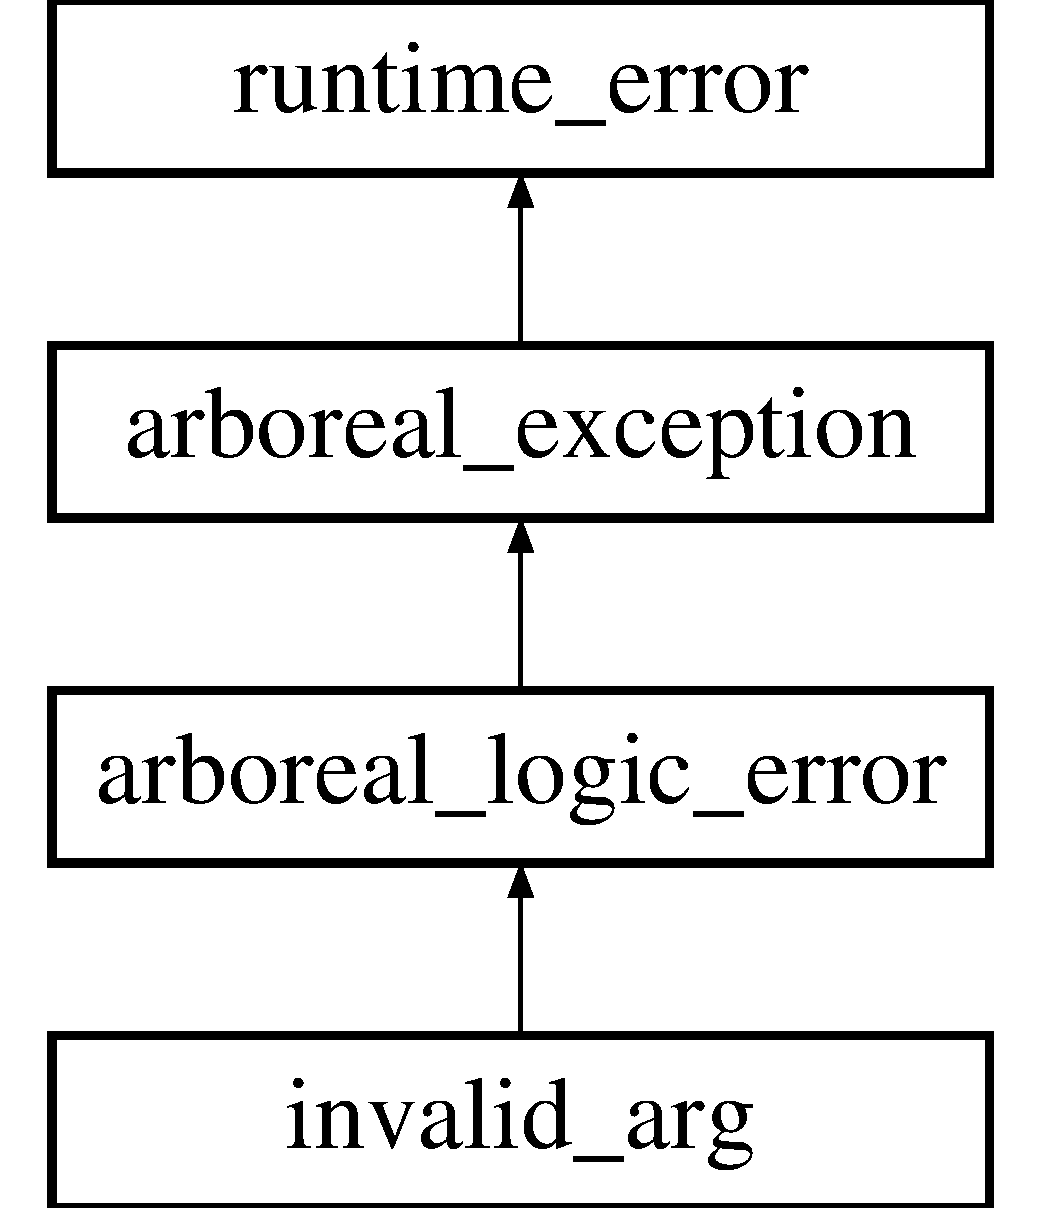
\includegraphics[height=4.000000cm]{classinvalid__arg}
\end{center}
\end{figure}
\subsection*{Public Member Functions}
\begin{DoxyCompactItemize}
\item 
{\bfseries invalid\+\_\+arg} (const char $\ast$what, const char $\ast$where, const int ecode=99)\hypertarget{classinvalid__arg_ab470c1e208290687c57ddb80ad7c91bf}{}\label{classinvalid__arg_ab470c1e208290687c57ddb80ad7c91bf}

\item 
{\bfseries invalid\+\_\+arg} (const char $\ast$what, const string \&where, const int ecode=99)\hypertarget{classinvalid__arg_ac64346933956c640dc48166d3c11ea6d}{}\label{classinvalid__arg_ac64346933956c640dc48166d3c11ea6d}

\item 
{\bfseries invalid\+\_\+arg} (const string \&what, const string \&where, const int ecode=99)\hypertarget{classinvalid__arg_afd1c07ada97de63dd8b2bf8d19753649}{}\label{classinvalid__arg_afd1c07ada97de63dd8b2bf8d19753649}

\item 
{\bfseries invalid\+\_\+arg} (const string \&what, const char $\ast$where, const int ecode=99)\hypertarget{classinvalid__arg_a1b68c46a8c2ddc202eb89edf05667618}{}\label{classinvalid__arg_a1b68c46a8c2ddc202eb89edf05667618}

\end{DoxyCompactItemize}
\subsection*{Additional Inherited Members}


The documentation for this class was generated from the following files\+:\begin{DoxyCompactItemize}
\item 
Shared\+Headers/Arboreal\+\_\+\+Exceptions.\+h\item 
Shared\+C\+P\+P\+Files/Arboreal\+\_\+\+Exceptions.\+cpp\end{DoxyCompactItemize}

\hypertarget{classModification}{}\section{Modification Class Reference}
\label{classModification}\index{Modification@{Modification}}
Inheritance diagram for Modification\+:\begin{figure}[H]
\begin{center}
\leavevmode
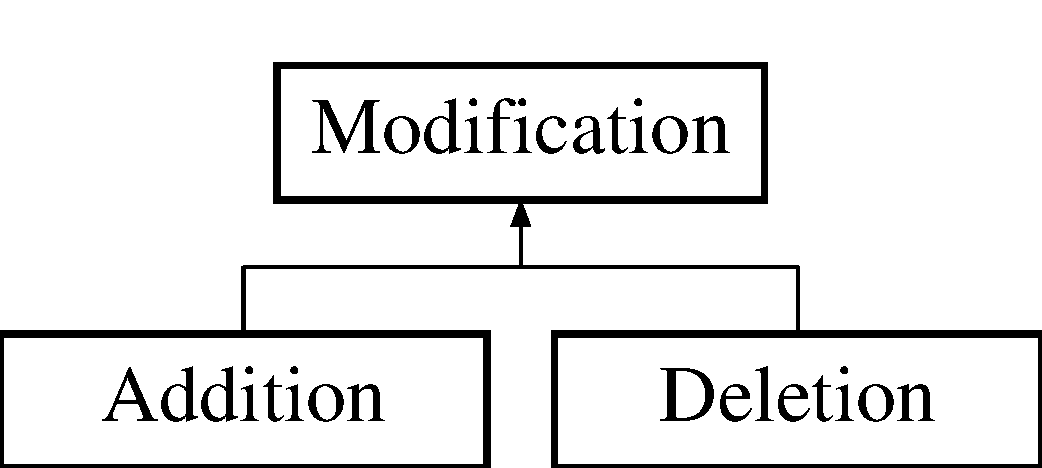
\includegraphics[height=2.000000cm]{classModification}
\end{center}
\end{figure}
\subsection*{Public Member Functions}
\begin{DoxyCompactItemize}
\item 
\mbox{\Hypertarget{classModification_a50d1fd809524902d2a1e78d02f4be1dc}\label{classModification_a50d1fd809524902d2a1e78d02f4be1dc}} 
virtual void {\bfseries write\+\_\+out} (\mbox{\hyperlink{classPartitionManager}{Partition\+Manager}} $\ast$pm)=0
\end{DoxyCompactItemize}
\subsection*{Protected Member Functions}
\begin{DoxyCompactItemize}
\item 
\mbox{\Hypertarget{classModification_a76407b8c6d2adb840dceea708355aba8}\label{classModification_a76407b8c6d2adb840dceea708355aba8}} 
{\bfseries Modification} (\mbox{\hyperlink{classTreeObject}{Tree\+Object}} $\ast$obj, \mbox{\hyperlink{classTreeObject}{Tree\+Object}} $\ast$parent)
\end{DoxyCompactItemize}
\subsection*{Protected Attributes}
\begin{DoxyCompactItemize}
\item 
\mbox{\Hypertarget{classModification_a0aa2f9924cde904b1683f3bd80d87a02}\label{classModification_a0aa2f9924cde904b1683f3bd80d87a02}} 
\mbox{\hyperlink{classTreeObject}{Tree\+Object}} $\ast$ {\bfseries \+\_\+mod}
\item 
\mbox{\Hypertarget{classModification_a529d02be9866b96746bcae63a763f868}\label{classModification_a529d02be9866b96746bcae63a763f868}} 
\mbox{\hyperlink{classTreeObject}{Tree\+Object}} $\ast$ {\bfseries \+\_\+parent}
\end{DoxyCompactItemize}


The documentation for this class was generated from the following files\+:\begin{DoxyCompactItemize}
\item 
Filesystem/\+Daemon\+Dependancies/\+Trees/Trees.\+h\item 
Filesystem/\+Daemon\+Dependancies/\+Trees/Trees.\+cpp\end{DoxyCompactItemize}

\hypertarget{classParseError}{}\section{Parse\+Error Class Reference}
\label{classParseError}\index{Parse\+Error@{Parse\+Error}}
\subsection*{Public Member Functions}
\begin{DoxyCompactItemize}
\item 
\mbox{\hyperlink{classParseError_a89210010aa80b9602ef5e57649886937}{Parse\+Error}} (const char $\ast$\mbox{\hyperlink{classParseError_aa725d47c84792c9142267e51c2074f58}{where}}, const char $\ast$\mbox{\hyperlink{classParseError_a08560dce27779ffee6c4bfb0d796aa6e}{what}})
\end{DoxyCompactItemize}
\begin{Indent}\textbf{ Accessor Functions}\par
\begin{DoxyCompactItemize}
\item 
std\+::string \mbox{\hyperlink{classParseError_aa725d47c84792c9142267e51c2074f58}{where}} ()
\item 
std\+::string \mbox{\hyperlink{classParseError_a08560dce27779ffee6c4bfb0d796aa6e}{what}} ()
\end{DoxyCompactItemize}
\end{Indent}


\subsection{Constructor \& Destructor Documentation}
\mbox{\Hypertarget{classParseError_a89210010aa80b9602ef5e57649886937}\label{classParseError_a89210010aa80b9602ef5e57649886937}} 
\index{Parse\+Error@{Parse\+Error}!Parse\+Error@{Parse\+Error}}
\index{Parse\+Error@{Parse\+Error}!Parse\+Error@{Parse\+Error}}
\subsubsection{\texorpdfstring{Parse\+Error()}{ParseError()}}
{\footnotesize\ttfamily Parse\+Error\+::\+Parse\+Error (\begin{DoxyParamCaption}\item[{const char $\ast$}]{where,  }\item[{const char $\ast$}]{what }\end{DoxyParamCaption})\hspace{0.3cm}{\ttfamily [inline]}}


\begin{DoxyParams}{Parameters}
{\em where} & Where the parse error took place\\
\hline
{\em what} & What the parse error consisted of \\
\hline
\end{DoxyParams}


\subsection{Member Function Documentation}
\mbox{\Hypertarget{classParseError_a08560dce27779ffee6c4bfb0d796aa6e}\label{classParseError_a08560dce27779ffee6c4bfb0d796aa6e}} 
\index{Parse\+Error@{Parse\+Error}!what@{what}}
\index{what@{what}!Parse\+Error@{Parse\+Error}}
\subsubsection{\texorpdfstring{what()}{what()}}
{\footnotesize\ttfamily std\+::string Parse\+Error\+::what (\begin{DoxyParamCaption}{ }\end{DoxyParamCaption})\hspace{0.3cm}{\ttfamily [inline]}}

\begin{DoxyReturn}{Returns}
A std\+::string detailing what the parse error consisted of 
\end{DoxyReturn}
\mbox{\Hypertarget{classParseError_aa725d47c84792c9142267e51c2074f58}\label{classParseError_aa725d47c84792c9142267e51c2074f58}} 
\index{Parse\+Error@{Parse\+Error}!where@{where}}
\index{where@{where}!Parse\+Error@{Parse\+Error}}
\subsubsection{\texorpdfstring{where()}{where()}}
{\footnotesize\ttfamily std\+::string Parse\+Error\+::where (\begin{DoxyParamCaption}{ }\end{DoxyParamCaption})\hspace{0.3cm}{\ttfamily [inline]}}

\begin{DoxyReturn}{Returns}
A std\+::string detailing where the parse error occured 
\end{DoxyReturn}


The documentation for this class was generated from the following file\+:\begin{DoxyCompactItemize}
\item 
C\+L\+I/Parser.\+h\end{DoxyCompactItemize}

\hypertarget{classParser}{}\section{Parser Class Reference}
\label{classParser}\index{Parser@{Parser}}
\subsection*{Public Member Functions}
\begin{DoxyCompactItemize}
\item 
\mbox{\hyperlink{classParser_a306c6c33d7a6cf1bb682be360fcfe982}{Parser}} (char $\ast$buffer, char $\ast$cwd, int max\+\_\+name\+\_\+size)
\item 
\mbox{\hyperlink{classParser_ada33680bf5f723ef95c44eeed1bff451}{Parser}} (std\+::string string, std\+::string cwd, int max\+\_\+name\+\_\+size)
\item 
\mbox{\hyperlink{classParser_a5168f5c44e9649e71796f9bef48bdbbe}{Parser}} (const char $\ast$string\+\_\+lit, const char $\ast$cwd, int max\+\_\+name\+\_\+size)
\item 
\mbox{\hyperlink{classParser_a12234f6cd36b61af4b50c94a179422c1}{Parser}} ()
\item 
\mbox{\hyperlink{classParser_a3e658b5917a93a3ef648050d060e3a93}{$\sim$\+Parser}} ()
\item 
void \mbox{\hyperlink{classParser_a87f5e73ca10ef5f84f37a4b37e0e6f59}{reset}} (std\+::string string, std\+::string cwd=\char`\"{}\char`\"{})
\begin{DoxyCompactList}\small\item\em Changes the member \+\_\+string of the parser class to whatever is passed. \end{DoxyCompactList}\item 
void \mbox{\hyperlink{classParser_a5e097c301e171481e8d2af91c112e35e}{reset}} (char $\ast$buffer, char $\ast$cwd=N\+U\+LL)
\begin{DoxyCompactList}\small\item\em Changes the member \+\_\+string of the parser class to whatever is passed. \end{DoxyCompactList}\item 
void \mbox{\hyperlink{classParser_ab51b81b1617f1948205d73804e3c0fb9}{reset}} (const char $\ast$string\+\_\+lit, const char $\ast$cwd=\char`\"{}\char`\"{})
\begin{DoxyCompactList}\small\item\em Changes the member \+\_\+string of the parser class to whatever is passed. \end{DoxyCompactList}\item 
void \mbox{\hyperlink{classParser_ac9c3bf43a7f27f92ecf538b83c5984d6}{set\+\_\+max\+\_\+name\+\_\+size}} (int size)
\begin{DoxyCompactList}\small\item\em Sets the maximum allowed file and tagname size that the \mbox{\hyperlink{classParser}{Parser}} will use. \end{DoxyCompactList}\item 
void \mbox{\hyperlink{classParser_a086f1431a0cac193fb6ff4506ba5c701}{set\+\_\+cwd}} (std\+::string cwd)
\begin{DoxyCompactList}\small\item\em Sets the Current Working Directory that the \mbox{\hyperlink{classParser}{Parser}} will use. \end{DoxyCompactList}\item 
std\+::vector$<$ std\+::string $>$ \mbox{\hyperlink{classParser_a5b531e9ed867eeb8ccb9cb088cf35c24}{parse}} (int type)
\begin{DoxyCompactList}\small\item\em Parse a string based on a certain rule. \end{DoxyCompactList}\item 
std\+::vector$<$ std\+::string $>$ \mbox{\hyperlink{classParser_aa973764b863dfbe448fa2fd7aa9ffdaa}{get\+\_\+cwd\+\_\+tags}} ()
\begin{DoxyCompactList}\small\item\em Returns a vector representation of the current working directory. \end{DoxyCompactList}\end{DoxyCompactItemize}
\subsection*{Static Public Member Functions}
\begin{DoxyCompactItemize}
\item 
static std\+::vector$<$ std\+::string $>$ \mbox{\hyperlink{classParser_a71c87961db9707dc18db00a645d3d1e5}{split\+\_\+on\+\_\+delim}} (std\+::string string, char delim)
\begin{DoxyCompactList}\small\item\em Splits a string at each instance of a particualar char (the delimeter) \end{DoxyCompactList}\end{DoxyCompactItemize}


\subsection{Constructor \& Destructor Documentation}
\mbox{\Hypertarget{classParser_a306c6c33d7a6cf1bb682be360fcfe982}\label{classParser_a306c6c33d7a6cf1bb682be360fcfe982}} 
\index{Parser@{Parser}!Parser@{Parser}}
\index{Parser@{Parser}!Parser@{Parser}}
\subsubsection{\texorpdfstring{Parser()}{Parser()}\hspace{0.1cm}{\footnotesize\ttfamily [1/4]}}
{\footnotesize\ttfamily Parser\+::\+Parser (\begin{DoxyParamCaption}\item[{char $\ast$}]{buffer,  }\item[{char $\ast$}]{cwd,  }\item[{int}]{max\+\_\+name\+\_\+size }\end{DoxyParamCaption})}


\begin{DoxyParams}{Parameters}
{\em buffer} & A C-\/\+Style String representation of the string to be parsed\\
\hline
{\em cwd} & A C-\/\+Style String representation of the current working directory; (This value is typically provided by the Liaison process). The directory string is used to parse commands which act within directories only thus providing commands such as \textquotesingle{}tag\textquotesingle{} a \char`\"{}path\char`\"{} to the file(s) which will be tagged without the user having to explicitly enter those file\textquotesingle{}s entire paths themselves.\\
\hline
{\em max\+\_\+name\+\_\+size} & The maximum length that a file or tagname is allowed to have; (This value is typically provided by the Liaison process) \\
\hline
\end{DoxyParams}
\mbox{\Hypertarget{classParser_ada33680bf5f723ef95c44eeed1bff451}\label{classParser_ada33680bf5f723ef95c44eeed1bff451}} 
\index{Parser@{Parser}!Parser@{Parser}}
\index{Parser@{Parser}!Parser@{Parser}}
\subsubsection{\texorpdfstring{Parser()}{Parser()}\hspace{0.1cm}{\footnotesize\ttfamily [2/4]}}
{\footnotesize\ttfamily Parser\+::\+Parser (\begin{DoxyParamCaption}\item[{std\+::string}]{string,  }\item[{std\+::string}]{cwd,  }\item[{int}]{max\+\_\+name\+\_\+size }\end{DoxyParamCaption})}


\begin{DoxyParams}{Parameters}
{\em buffer} & A std\+::string representation of the string to be parsed\\
\hline
{\em cwd} & A std\+::string representation of the current working directory; (This value is typically provided by the Liaison process). The directory string is used to parse commands which act within directories only thus, providing commands such as \textquotesingle{}tag\textquotesingle{} a \char`\"{}path\char`\"{} to the file(s) which will be tagged without the user having to explicitly enter those file\textquotesingle{}s entire paths themselves.\\
\hline
{\em max\+\_\+name\+\_\+size} & The maximum length that a file or tagname is allowed to have; (This value is typically provided by the Liaison process) \\
\hline
\end{DoxyParams}
\mbox{\Hypertarget{classParser_a5168f5c44e9649e71796f9bef48bdbbe}\label{classParser_a5168f5c44e9649e71796f9bef48bdbbe}} 
\index{Parser@{Parser}!Parser@{Parser}}
\index{Parser@{Parser}!Parser@{Parser}}
\subsubsection{\texorpdfstring{Parser()}{Parser()}\hspace{0.1cm}{\footnotesize\ttfamily [3/4]}}
{\footnotesize\ttfamily Parser\+::\+Parser (\begin{DoxyParamCaption}\item[{const char $\ast$}]{string\+\_\+lit,  }\item[{const char $\ast$}]{cwd,  }\item[{int}]{max\+\_\+name\+\_\+size }\end{DoxyParamCaption})}


\begin{DoxyParams}{Parameters}
{\em buffer} & A String Literal representation of the string to be parsed\\
\hline
{\em cwd} & A String Literal representation of the current working directory; (This value is typically provided by the Liaison process). The directory string is used to parse commands which act within directories only thus, providing commands such as \textquotesingle{}tag\textquotesingle{} a \char`\"{}path\char`\"{} to the file(s) which will be tagged without the user having to explicitly enter those file\textquotesingle{}s entire paths themselves.\\
\hline
{\em max\+\_\+name\+\_\+size} & The maximum length that a file or tagname is allowed to have; (This value is typically provided by the Liaison process) \\
\hline
\end{DoxyParams}
\mbox{\Hypertarget{classParser_a12234f6cd36b61af4b50c94a179422c1}\label{classParser_a12234f6cd36b61af4b50c94a179422c1}} 
\index{Parser@{Parser}!Parser@{Parser}}
\index{Parser@{Parser}!Parser@{Parser}}
\subsubsection{\texorpdfstring{Parser()}{Parser()}\hspace{0.1cm}{\footnotesize\ttfamily [4/4]}}
{\footnotesize\ttfamily Parser\+::\+Parser (\begin{DoxyParamCaption}{ }\end{DoxyParamCaption})}

Default Constructor to be used in case initialization of values needs to be done elsewhere \mbox{\Hypertarget{classParser_a3e658b5917a93a3ef648050d060e3a93}\label{classParser_a3e658b5917a93a3ef648050d060e3a93}} 
\index{Parser@{Parser}!````~Parser@{$\sim$\+Parser}}
\index{````~Parser@{$\sim$\+Parser}!Parser@{Parser}}
\subsubsection{\texorpdfstring{$\sim$\+Parser()}{~Parser()}}
{\footnotesize\ttfamily Parser\+::$\sim$\+Parser (\begin{DoxyParamCaption}{ }\end{DoxyParamCaption})}

Default Destructor; Does nothing 

\subsection{Member Function Documentation}
\mbox{\Hypertarget{classParser_aa973764b863dfbe448fa2fd7aa9ffdaa}\label{classParser_aa973764b863dfbe448fa2fd7aa9ffdaa}} 
\index{Parser@{Parser}!get\+\_\+cwd\+\_\+tags@{get\+\_\+cwd\+\_\+tags}}
\index{get\+\_\+cwd\+\_\+tags@{get\+\_\+cwd\+\_\+tags}!Parser@{Parser}}
\subsubsection{\texorpdfstring{get\+\_\+cwd\+\_\+tags()}{get\_cwd\_tags()}}
{\footnotesize\ttfamily std\+::vector$<$ std\+::string $>$ Parser\+::get\+\_\+cwd\+\_\+tags (\begin{DoxyParamCaption}{ }\end{DoxyParamCaption})}



Returns a vector representation of the current working directory. 

That is, it will decompose \textquotesingle{}/string1/string2\textquotesingle{} into a vector containing \mbox{[}string1, string2\mbox{]}. This is useful when the calling code requires the current working directory as a vector of strings rather than as a standard string representation.

\begin{DoxyReturn}{Returns}
A std\+::vector of std\+::string comprised of the non-\/\textquotesingle{}/\textquotesingle{} parts of the \mbox{\hyperlink{classParser}{Parser}} member value \+\_\+cwd 
\end{DoxyReturn}
\mbox{\Hypertarget{classParser_a5b531e9ed867eeb8ccb9cb088cf35c24}\label{classParser_a5b531e9ed867eeb8ccb9cb088cf35c24}} 
\index{Parser@{Parser}!parse@{parse}}
\index{parse@{parse}!Parser@{Parser}}
\subsubsection{\texorpdfstring{parse()}{parse()}}
{\footnotesize\ttfamily std\+::vector$<$ std\+::string $>$ Parser\+::parse (\begin{DoxyParamCaption}\item[{int}]{type }\end{DoxyParamCaption})}



Parse a string based on a certain rule. 

The rule generally corresponds to how a \mbox{\hyperlink{classCLI}{C\+LI}} command should be decomposed. ~\newline
For example the \mbox{\hyperlink{classCLI}{C\+LI}} command for finding files takes a list of files, hower the filesystem itself does not support batch commands, therefore, the \mbox{\hyperlink{classParser}{Parser}} will decompose the command into its constituent parts (i.\+e. a single file). ~\newline
This particular behavior is access by passing \textquotesingle{}8\textquotesingle{} as the \char`\"{}type\char`\"{} of decomposition that needs to take place (Note that this corresponds to the command\textquotesingle{}s ID). ~\newline
However the \mbox{\hyperlink{classParser}{Parser}} can be extended to support any rule whatsoever, so long as it is added to the \mbox{\hyperlink{classParser}{Parser}}\textquotesingle{}s \mbox{\hyperlink{classParser_a5b531e9ed867eeb8ccb9cb088cf35c24}{parse()}} function switch statement.


\begin{DoxyParams}{Parameters}
{\em type} & The integer identification of the parse rule that will be executed\\
\hline
\end{DoxyParams}
\begin{DoxyReturn}{Returns}
A std\+::vector of std\+::string comprised of the result after the chosen parse rule is executed. 
\end{DoxyReturn}
\mbox{\Hypertarget{classParser_a87f5e73ca10ef5f84f37a4b37e0e6f59}\label{classParser_a87f5e73ca10ef5f84f37a4b37e0e6f59}} 
\index{Parser@{Parser}!reset@{reset}}
\index{reset@{reset}!Parser@{Parser}}
\subsubsection{\texorpdfstring{reset()}{reset()}\hspace{0.1cm}{\footnotesize\ttfamily [1/3]}}
{\footnotesize\ttfamily void Parser\+::reset (\begin{DoxyParamCaption}\item[{std\+::string}]{string,  }\item[{std\+::string}]{cwd = {\ttfamily \char`\"{}\char`\"{}} }\end{DoxyParamCaption})}



Changes the member \+\_\+string of the parser class to whatever is passed. 

The \mbox{\hyperlink{classParser}{Parser}} class conducts all operations on its member \+\_\+string rather than requiring that a string value be passed to its \mbox{\hyperlink{classParser_a5b531e9ed867eeb8ccb9cb088cf35c24}{parse()}} method. This was done in order to make use of the class as streamlined as possible.


\begin{DoxyParams}{Parameters}
{\em string} & A std\+::string representation of the string to be parsed\\
\hline
{\em cwd} & A std\+::string representation of the current working directory; Note that this argument is optional and allows the user to both reset the string the \mbox{\hyperlink{classParser}{Parser}} will work with as well as the directory string the \mbox{\hyperlink{classParser}{Parser}} will use. The directory string is used to parse commands which act within directories only thus providing commands such as \textquotesingle{}tag\textquotesingle{} a \char`\"{}path\char`\"{} to the file(s) which will be tagged without the user having to explicitly enter those file\textquotesingle{}s entire paths themselves. \\
\hline
\end{DoxyParams}
\mbox{\Hypertarget{classParser_a5e097c301e171481e8d2af91c112e35e}\label{classParser_a5e097c301e171481e8d2af91c112e35e}} 
\index{Parser@{Parser}!reset@{reset}}
\index{reset@{reset}!Parser@{Parser}}
\subsubsection{\texorpdfstring{reset()}{reset()}\hspace{0.1cm}{\footnotesize\ttfamily [2/3]}}
{\footnotesize\ttfamily void Parser\+::reset (\begin{DoxyParamCaption}\item[{char $\ast$}]{buffer,  }\item[{char $\ast$}]{cwd = {\ttfamily NULL} }\end{DoxyParamCaption})}



Changes the member \+\_\+string of the parser class to whatever is passed. 

The \mbox{\hyperlink{classParser}{Parser}} class conducts all operations on its member \+\_\+string rather than requiring that a string value be passed to its \mbox{\hyperlink{classParser_a5b531e9ed867eeb8ccb9cb088cf35c24}{parse()}} method. This was done in order to make use of the class as streamlined as possible.


\begin{DoxyParams}{Parameters}
{\em string} & A C-\/\+Style String representation of the string to be parsed\\
\hline
{\em cwd} & A C-\/\+Style String representation of the current working directory; Note that this argument is optional and allows the user to both reset the string the \mbox{\hyperlink{classParser}{Parser}} will work with as well as the directory string the \mbox{\hyperlink{classParser}{Parser}} will use. The directory string is used to parse commands which act within directories only thus providing commands such as \textquotesingle{}tag\textquotesingle{} a \char`\"{}path\char`\"{} to the file(s) which will be tagged without the user having to explicitly enter those file\textquotesingle{}s entire paths themselves.\\
\hline
\end{DoxyParams}
\begin{DoxyReturn}{Returns}
Void 
\end{DoxyReturn}
\mbox{\Hypertarget{classParser_ab51b81b1617f1948205d73804e3c0fb9}\label{classParser_ab51b81b1617f1948205d73804e3c0fb9}} 
\index{Parser@{Parser}!reset@{reset}}
\index{reset@{reset}!Parser@{Parser}}
\subsubsection{\texorpdfstring{reset()}{reset()}\hspace{0.1cm}{\footnotesize\ttfamily [3/3]}}
{\footnotesize\ttfamily void Parser\+::reset (\begin{DoxyParamCaption}\item[{const char $\ast$}]{string\+\_\+lit,  }\item[{const char $\ast$}]{cwd = {\ttfamily \char`\"{}\char`\"{}} }\end{DoxyParamCaption})}



Changes the member \+\_\+string of the parser class to whatever is passed. 

The \mbox{\hyperlink{classParser}{Parser}} class conducts all operations on its member \+\_\+string rather than requiring that a string value be passed to its \mbox{\hyperlink{classParser_a5b531e9ed867eeb8ccb9cb088cf35c24}{parse()}} method. This was done in order to make use of the class as streamlined as possible.


\begin{DoxyParams}{Parameters}
{\em string} & A String Literal representation of the string to be parsed\\
\hline
{\em cwd} & A String Literal representation of the current working directory; Note that this argument is optional and allows the user to both reset the string the \mbox{\hyperlink{classParser}{Parser}} will work with as well as the directory string the \mbox{\hyperlink{classParser}{Parser}} will use. The directory string is used to parse commands which act within directories only thus providing commands such as \textquotesingle{}tag\textquotesingle{} a \char`\"{}path\char`\"{} to the file(s) which will be tagged without the user having to explicitly enter those file\textquotesingle{}s entire paths themselves.\\
\hline
\end{DoxyParams}
\begin{DoxyReturn}{Returns}
Void 
\end{DoxyReturn}
\mbox{\Hypertarget{classParser_a086f1431a0cac193fb6ff4506ba5c701}\label{classParser_a086f1431a0cac193fb6ff4506ba5c701}} 
\index{Parser@{Parser}!set\+\_\+cwd@{set\+\_\+cwd}}
\index{set\+\_\+cwd@{set\+\_\+cwd}!Parser@{Parser}}
\subsubsection{\texorpdfstring{set\+\_\+cwd()}{set\_cwd()}}
{\footnotesize\ttfamily void Parser\+::set\+\_\+cwd (\begin{DoxyParamCaption}\item[{std\+::string}]{cwd }\end{DoxyParamCaption})}



Sets the Current Working Directory that the \mbox{\hyperlink{classParser}{Parser}} will use. 

The directory string is used to parse commands which act within directories only thus providing commands such as \textquotesingle{}tag\textquotesingle{} a \char`\"{}path\char`\"{} to the file(s) which will be tagged without the user having to explicitly enter those file\textquotesingle{}s entire paths themselves. This function does not have counterparts which tahe C-\/\+Style Strings or String Literals. This is because, in all situations, if the current working directory must be set using this method, it is highly likely that the calling code has a std\+::string representation of the current working directory rather than a representation in one of the other formats. If such functionality (C-\/\+Style Strings and others) is desired, extensibility is easy enough. Regardless the \mbox{\hyperlink{classParser}{Parser}}\textquotesingle{}s \+\_\+cwd member will always be a std\+::string.


\begin{DoxyParams}{Parameters}
{\em cwd} & A std\+::string representation of the current working directory\\
\hline
\end{DoxyParams}
\begin{DoxyReturn}{Returns}
Void 
\end{DoxyReturn}
\mbox{\Hypertarget{classParser_ac9c3bf43a7f27f92ecf538b83c5984d6}\label{classParser_ac9c3bf43a7f27f92ecf538b83c5984d6}} 
\index{Parser@{Parser}!set\+\_\+max\+\_\+name\+\_\+size@{set\+\_\+max\+\_\+name\+\_\+size}}
\index{set\+\_\+max\+\_\+name\+\_\+size@{set\+\_\+max\+\_\+name\+\_\+size}!Parser@{Parser}}
\subsubsection{\texorpdfstring{set\+\_\+max\+\_\+name\+\_\+size()}{set\_max\_name\_size()}}
{\footnotesize\ttfamily void Parser\+::set\+\_\+max\+\_\+name\+\_\+size (\begin{DoxyParamCaption}\item[{int}]{size }\end{DoxyParamCaption})}



Sets the maximum allowed file and tagname size that the \mbox{\hyperlink{classParser}{Parser}} will use. 

If this size is exceeded an error is thrown and the \mbox{\hyperlink{classParser}{Parser}} will stop its current activities. This value is dictated by the \mbox{\hyperlink{classCLI}{C\+LI}} and is generally provided to the \mbox{\hyperlink{classParser}{Parser}} by the Liaison Process.


\begin{DoxyParams}{Parameters}
{\em size} & The maximum file/tag name length \\
\hline
\end{DoxyParams}
\mbox{\Hypertarget{classParser_a71c87961db9707dc18db00a645d3d1e5}\label{classParser_a71c87961db9707dc18db00a645d3d1e5}} 
\index{Parser@{Parser}!split\+\_\+on\+\_\+delim@{split\+\_\+on\+\_\+delim}}
\index{split\+\_\+on\+\_\+delim@{split\+\_\+on\+\_\+delim}!Parser@{Parser}}
\subsubsection{\texorpdfstring{split\+\_\+on\+\_\+delim()}{split\_on\_delim()}}
{\footnotesize\ttfamily std\+::vector$<$ std\+::string $>$ Parser\+::split\+\_\+on\+\_\+delim (\begin{DoxyParamCaption}\item[{std\+::string}]{string,  }\item[{char}]{delim }\end{DoxyParamCaption})\hspace{0.3cm}{\ttfamily [static]}}



Splits a string at each instance of a particualar char (the delimeter) 

The delimeters are N\+OT included anywhere in the resulting vector. This function is static and is mainly used outside the \mbox{\hyperlink{classParser}{Parser}} in order to split values that the parser returned. This can happen because the complexity of certain commands does not allow the parser to fully decompose the string and instead it can only reorganize the command into a form which can be easily split later. It is important to note that this function does not differentiate between the number of delimeter charcters the string contains. That is, it will read the whole string and split it at any point where the delimeter is seen whether it is seen in 1 or 100 places.


\begin{DoxyParams}{Parameters}
{\em string} & A std\+::string representation of whatever string needs to be split \\
\hline
{\em delim} & A char value representing where the string should be split \\
\hline
\end{DoxyParams}


The documentation for this class was generated from the following files\+:\begin{DoxyCompactItemize}
\item 
Shared\+Headers/Parser.\+h\item 
Shared\+C\+P\+P\+Files/Parser.\+cpp\end{DoxyCompactItemize}

\hypertarget{classPartitionManager}{}\section{Partition\+Manager Class Reference}
\label{classPartitionManager}\index{Partition\+Manager@{Partition\+Manager}}
\subsection*{Public Member Functions}
\begin{DoxyCompactItemize}
\item 
\mbox{\hyperlink{classPartitionManager_aa875b0b19b7ab9f32b02d2c9be383b75}{Partition\+Manager}} (\mbox{\hyperlink{classDiskManager}{Disk\+Manager}} $\ast$dm, string partition\+Name)
\end{DoxyCompactItemize}
\begin{Indent}\textbf{ Accessor Functions}\par
\begin{DoxyCompactItemize}
\item 
void \mbox{\hyperlink{classPartitionManager_a7aca34c24770b7b9290c489475655ada}{read\+Disk\+Block}} (Blk\+Num\+Type blknum, char $\ast$blkdata)
\item 
size\+\_\+t \mbox{\hyperlink{classPartitionManager_aa1026e17e77f154d7034fafd188bda02}{get\+Block\+Size}} ()
\item 
string \mbox{\hyperlink{classPartitionManager_a7c756dba2665e5a7b62b2ccb261f1158}{get\+Partition\+Name}} ()
\item 
int \mbox{\hyperlink{classPartitionManager_a3b047c1c63c2f9a9e04805471c04ccf0}{get\+\_\+file\+\_\+name\+\_\+size}} ()
\end{DoxyCompactItemize}
\end{Indent}
\begin{Indent}\textbf{ Modifier Functions}\par
\begin{DoxyCompactItemize}
\item 
void \mbox{\hyperlink{classPartitionManager_a114d5d4f8d90b6e9207b09d99e246bed}{write\+Disk\+Block}} (Blk\+Num\+Type blknum, char $\ast$blkdata)
\item 
Blk\+Num\+Type \mbox{\hyperlink{classPartitionManager_a682ce5963a31cf7009455cb1c229b26a}{get\+Free\+Disk\+Block}} ()
\item 
void \mbox{\hyperlink{classPartitionManager_a3ce9b50aa5e7d9063919fc55d125246b}{return\+Disk\+Block}} (Blk\+Num\+Type blknum)
\end{DoxyCompactItemize}
\end{Indent}


\subsection{Constructor \& Destructor Documentation}
\mbox{\Hypertarget{classPartitionManager_aa875b0b19b7ab9f32b02d2c9be383b75}\label{classPartitionManager_aa875b0b19b7ab9f32b02d2c9be383b75}} 
\index{Partition\+Manager@{Partition\+Manager}!Partition\+Manager@{Partition\+Manager}}
\index{Partition\+Manager@{Partition\+Manager}!Partition\+Manager@{Partition\+Manager}}
\subsubsection{\texorpdfstring{Partition\+Manager()}{PartitionManager()}}
{\footnotesize\ttfamily Partition\+Manager\+::\+Partition\+Manager (\begin{DoxyParamCaption}\item[{\mbox{\hyperlink{classDiskManager}{Disk\+Manager}} $\ast$}]{dm,  }\item[{string}]{partition\+Name }\end{DoxyParamCaption})}


\begin{DoxyParams}{Parameters}
{\em dm} & the \mbox{\hyperlink{classDiskManager}{Disk\+Manager}} associated with this object \\
\hline
{\em partition\+Name} & the name of the partition that this will be managing \\
\hline
\end{DoxyParams}


\subsection{Member Function Documentation}
\mbox{\Hypertarget{classPartitionManager_a3b047c1c63c2f9a9e04805471c04ccf0}\label{classPartitionManager_a3b047c1c63c2f9a9e04805471c04ccf0}} 
\index{Partition\+Manager@{Partition\+Manager}!get\+\_\+file\+\_\+name\+\_\+size@{get\+\_\+file\+\_\+name\+\_\+size}}
\index{get\+\_\+file\+\_\+name\+\_\+size@{get\+\_\+file\+\_\+name\+\_\+size}!Partition\+Manager@{Partition\+Manager}}
\subsubsection{\texorpdfstring{get\+\_\+file\+\_\+name\+\_\+size()}{get\_file\_name\_size()}}
{\footnotesize\ttfamily int Partition\+Manager\+::get\+\_\+file\+\_\+name\+\_\+size (\begin{DoxyParamCaption}{ }\end{DoxyParamCaption})}

\begin{DoxyReturn}{Returns}
The maximum file name size for this partition in bytes 
\end{DoxyReturn}
\mbox{\Hypertarget{classPartitionManager_aa1026e17e77f154d7034fafd188bda02}\label{classPartitionManager_aa1026e17e77f154d7034fafd188bda02}} 
\index{Partition\+Manager@{Partition\+Manager}!get\+Block\+Size@{get\+Block\+Size}}
\index{get\+Block\+Size@{get\+Block\+Size}!Partition\+Manager@{Partition\+Manager}}
\subsubsection{\texorpdfstring{get\+Block\+Size()}{getBlockSize()}}
{\footnotesize\ttfamily size\+\_\+t Partition\+Manager\+::get\+Block\+Size (\begin{DoxyParamCaption}{ }\end{DoxyParamCaption})}

\begin{DoxyReturn}{Returns}
the blocksize of the \mbox{\hyperlink{classDisk}{Disk}} 
\end{DoxyReturn}
\mbox{\Hypertarget{classPartitionManager_a682ce5963a31cf7009455cb1c229b26a}\label{classPartitionManager_a682ce5963a31cf7009455cb1c229b26a}} 
\index{Partition\+Manager@{Partition\+Manager}!get\+Free\+Disk\+Block@{get\+Free\+Disk\+Block}}
\index{get\+Free\+Disk\+Block@{get\+Free\+Disk\+Block}!Partition\+Manager@{Partition\+Manager}}
\subsubsection{\texorpdfstring{get\+Free\+Disk\+Block()}{getFreeDiskBlock()}}
{\footnotesize\ttfamily Blk\+Num\+Type Partition\+Manager\+::get\+Free\+Disk\+Block (\begin{DoxyParamCaption}{ }\end{DoxyParamCaption})}

Allocates a block on disk if there is a free one. The \mbox{\hyperlink{classDisk}{Disk}} free list is updated accordingly \begin{DoxyReturn}{Returns}
the block number of the newly allocated block 
\end{DoxyReturn}
\mbox{\Hypertarget{classPartitionManager_a7c756dba2665e5a7b62b2ccb261f1158}\label{classPartitionManager_a7c756dba2665e5a7b62b2ccb261f1158}} 
\index{Partition\+Manager@{Partition\+Manager}!get\+Partition\+Name@{get\+Partition\+Name}}
\index{get\+Partition\+Name@{get\+Partition\+Name}!Partition\+Manager@{Partition\+Manager}}
\subsubsection{\texorpdfstring{get\+Partition\+Name()}{getPartitionName()}}
{\footnotesize\ttfamily string Partition\+Manager\+::get\+Partition\+Name (\begin{DoxyParamCaption}{ }\end{DoxyParamCaption})}

\begin{DoxyReturn}{Returns}
The name of the partition this \mbox{\hyperlink{classPartitionManager}{Partition\+Manager}} is associated with 
\end{DoxyReturn}
\mbox{\Hypertarget{classPartitionManager_a7aca34c24770b7b9290c489475655ada}\label{classPartitionManager_a7aca34c24770b7b9290c489475655ada}} 
\index{Partition\+Manager@{Partition\+Manager}!read\+Disk\+Block@{read\+Disk\+Block}}
\index{read\+Disk\+Block@{read\+Disk\+Block}!Partition\+Manager@{Partition\+Manager}}
\subsubsection{\texorpdfstring{read\+Disk\+Block()}{readDiskBlock()}}
{\footnotesize\ttfamily void Partition\+Manager\+::read\+Disk\+Block (\begin{DoxyParamCaption}\item[{Blk\+Num\+Type}]{blknum,  }\item[{char $\ast$}]{blkdata }\end{DoxyParamCaption})}

Reads a block from the \mbox{\hyperlink{classDisk}{Disk}}. 
\begin{DoxyParams}{Parameters}
{\em blknum} & the blocknumber to be read \\
\hline
{\em blkdata} & the buffer to put the read data. must be large enough to contain an entire block of data \\
\hline
\end{DoxyParams}
\mbox{\Hypertarget{classPartitionManager_a3ce9b50aa5e7d9063919fc55d125246b}\label{classPartitionManager_a3ce9b50aa5e7d9063919fc55d125246b}} 
\index{Partition\+Manager@{Partition\+Manager}!return\+Disk\+Block@{return\+Disk\+Block}}
\index{return\+Disk\+Block@{return\+Disk\+Block}!Partition\+Manager@{Partition\+Manager}}
\subsubsection{\texorpdfstring{return\+Disk\+Block()}{returnDiskBlock()}}
{\footnotesize\ttfamily void Partition\+Manager\+::return\+Disk\+Block (\begin{DoxyParamCaption}\item[{Blk\+Num\+Type}]{blknum }\end{DoxyParamCaption})}

returns a block to the \mbox{\hyperlink{classDisk}{Disk}} free list and zeros it out before writing. 
\begin{DoxyParams}{Parameters}
{\em blknum} & the blocknumber of the block to be freed \\
\hline
\end{DoxyParams}
\mbox{\Hypertarget{classPartitionManager_a114d5d4f8d90b6e9207b09d99e246bed}\label{classPartitionManager_a114d5d4f8d90b6e9207b09d99e246bed}} 
\index{Partition\+Manager@{Partition\+Manager}!write\+Disk\+Block@{write\+Disk\+Block}}
\index{write\+Disk\+Block@{write\+Disk\+Block}!Partition\+Manager@{Partition\+Manager}}
\subsubsection{\texorpdfstring{write\+Disk\+Block()}{writeDiskBlock()}}
{\footnotesize\ttfamily void Partition\+Manager\+::write\+Disk\+Block (\begin{DoxyParamCaption}\item[{Blk\+Num\+Type}]{blknum,  }\item[{char $\ast$}]{blkdata }\end{DoxyParamCaption})}

Writes a block to the \mbox{\hyperlink{classDisk}{Disk}}. 
\begin{DoxyParams}{Parameters}
{\em blknum} & the blocknumber to be written \\
\hline
{\em blkdata} & the buffer to write the data from. It Will write an entire block size of data. \\
\hline
\end{DoxyParams}


The documentation for this class was generated from the following files\+:\begin{DoxyCompactItemize}
\item 
Filesystem/\+Daemon\+Dependancies/\+Partition\+Manager/Partition\+Manager.\+h\item 
Filesystem/\+Daemon\+Dependancies/\+Partition\+Manager/Partition\+Manager.\+cpp\end{DoxyCompactItemize}

\hypertarget{structrootSuperBlock}{}\section{root\+Super\+Block Struct Reference}
\label{structrootSuperBlock}\index{root\+Super\+Block@{root\+Super\+Block}}
\subsection*{Public Attributes}
\begin{DoxyCompactItemize}
\item 
\mbox{\Hypertarget{structrootSuperBlock_a346c6cd3ede82eb90190548d45c1789d}\label{structrootSuperBlock_a346c6cd3ede82eb90190548d45c1789d}} 
size\+\_\+t {\bfseries size}
\item 
\mbox{\Hypertarget{structrootSuperBlock_ac316fdcc2d2736d675980495d1732872}\label{structrootSuperBlock_ac316fdcc2d2736d675980495d1732872}} 
\mbox{\hyperlink{structindex}{Index}} {\bfseries last\+Entry}
\item 
\mbox{\Hypertarget{structrootSuperBlock_afb7d56b6d69b3f1555db0e3bce1d9612}\label{structrootSuperBlock_afb7d56b6d69b3f1555db0e3bce1d9612}} 
Blk\+Num\+Type {\bfseries start\+Block}
\end{DoxyCompactItemize}


The documentation for this struct was generated from the following file\+:\begin{DoxyCompactItemize}
\item 
Filesystem/types.\+h\end{DoxyCompactItemize}

\hypertarget{classRootTree}{}\section{Root\+Tree Class Reference}
\label{classRootTree}\index{Root\+Tree@{Root\+Tree}}
Inheritance diagram for Root\+Tree\+:\begin{figure}[H]
\begin{center}
\leavevmode
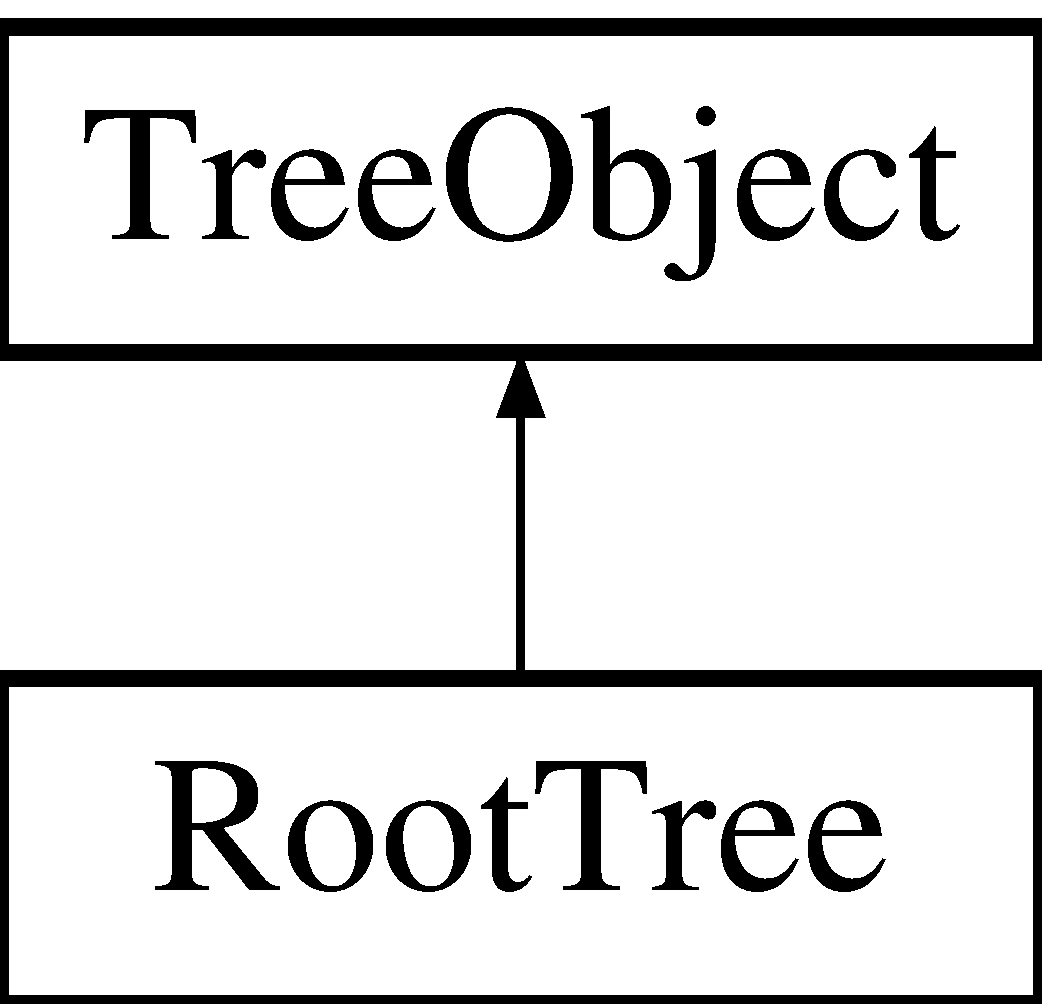
\includegraphics[height=2.000000cm]{classRootTree}
\end{center}
\end{figure}
\subsection*{Public Member Functions}
\begin{DoxyCompactItemize}
\item 
\mbox{\Hypertarget{classRootTree_a491c0374c9024faf1e1c8045f21a4cad}\label{classRootTree_a491c0374c9024faf1e1c8045f21a4cad}} 
{\bfseries Root\+Tree} (\mbox{\hyperlink{classPartitionManager}{Partition\+Manager}} $\ast$pm)
\item 
void \mbox{\hyperlink{classRootTree_ad6eefe5d46ee37b3725799897a78c2dd}{write\+\_\+out}} ()
\item 
void \mbox{\hyperlink{classRootTree_a658eed78be67e890de2283af960dc532}{read\+\_\+in}} (unordered\+\_\+multimap$<$ string, \mbox{\hyperlink{classFileInfo}{File\+Info}} $\ast$$>$ $\ast$all\+Files, \mbox{\hyperlink{classRootTree}{Root\+Tree}} $\ast$root\+Tree)
\item 
void \mbox{\hyperlink{classRootTree_ac431dc04b767fc66791c251d8173650d}{del}} ()
\end{DoxyCompactItemize}
\subsection*{Additional Inherited Members}


\subsection{Member Function Documentation}
\mbox{\Hypertarget{classRootTree_ac431dc04b767fc66791c251d8173650d}\label{classRootTree_ac431dc04b767fc66791c251d8173650d}} 
\index{Root\+Tree@{Root\+Tree}!del@{del}}
\index{del@{del}!Root\+Tree@{Root\+Tree}}
\subsubsection{\texorpdfstring{del()}{del()}}
{\footnotesize\ttfamily void Root\+Tree\+::del (\begin{DoxyParamCaption}{ }\end{DoxyParamCaption})\hspace{0.3cm}{\ttfamily [virtual]}}

Will completely remove the \mbox{\hyperlink{classTreeObject}{Tree\+Object}}\textquotesingle{}s presence on disk 

Implements \mbox{\hyperlink{classTreeObject_af390b7479aa972888e594c07a85740b6}{Tree\+Object}}.

\mbox{\Hypertarget{classRootTree_a658eed78be67e890de2283af960dc532}\label{classRootTree_a658eed78be67e890de2283af960dc532}} 
\index{Root\+Tree@{Root\+Tree}!read\+\_\+in@{read\+\_\+in}}
\index{read\+\_\+in@{read\+\_\+in}!Root\+Tree@{Root\+Tree}}
\subsubsection{\texorpdfstring{read\+\_\+in()}{read\_in()}}
{\footnotesize\ttfamily void Root\+Tree\+::read\+\_\+in (\begin{DoxyParamCaption}\item[{unordered\+\_\+multimap$<$ string, \mbox{\hyperlink{classFileInfo}{File\+Info}} $\ast$$>$ $\ast$}]{all\+Files,  }\item[{\mbox{\hyperlink{classRootTree}{Root\+Tree}} $\ast$}]{root\+Tree }\end{DoxyParamCaption})\hspace{0.3cm}{\ttfamily [virtual]}}

Will read in all object data from disk 
\begin{DoxyParams}{Parameters}
{\em all\+Files} & a pointer to the map of all files \\
\hline
{\em root\+Tree} & a pointer to the root tree \\
\hline
\end{DoxyParams}


Implements \mbox{\hyperlink{classTreeObject_a722eb00e6782626281afc8eff92840a4}{Tree\+Object}}.

\mbox{\Hypertarget{classRootTree_ad6eefe5d46ee37b3725799897a78c2dd}\label{classRootTree_ad6eefe5d46ee37b3725799897a78c2dd}} 
\index{Root\+Tree@{Root\+Tree}!write\+\_\+out@{write\+\_\+out}}
\index{write\+\_\+out@{write\+\_\+out}!Root\+Tree@{Root\+Tree}}
\subsubsection{\texorpdfstring{write\+\_\+out()}{write\_out()}}
{\footnotesize\ttfamily void Root\+Tree\+::write\+\_\+out (\begin{DoxyParamCaption}{ }\end{DoxyParamCaption})\hspace{0.3cm}{\ttfamily [virtual]}}

Intended to write out the object to disk 

Implements \mbox{\hyperlink{classTreeObject_a63708d61353d83e3e03597394bb7aca0}{Tree\+Object}}.



The documentation for this class was generated from the following files\+:\begin{DoxyCompactItemize}
\item 
Filesystem/\+Backend/Trees.\+h\item 
Filesystem/\+Backend/Trees.\+cpp\end{DoxyCompactItemize}

\hypertarget{classtag__error}{}\section{tag\+\_\+error Class Reference}
\label{classtag__error}\index{tag\+\_\+error@{tag\+\_\+error}}
Inheritance diagram for tag\+\_\+error\+:\begin{figure}[H]
\begin{center}
\leavevmode
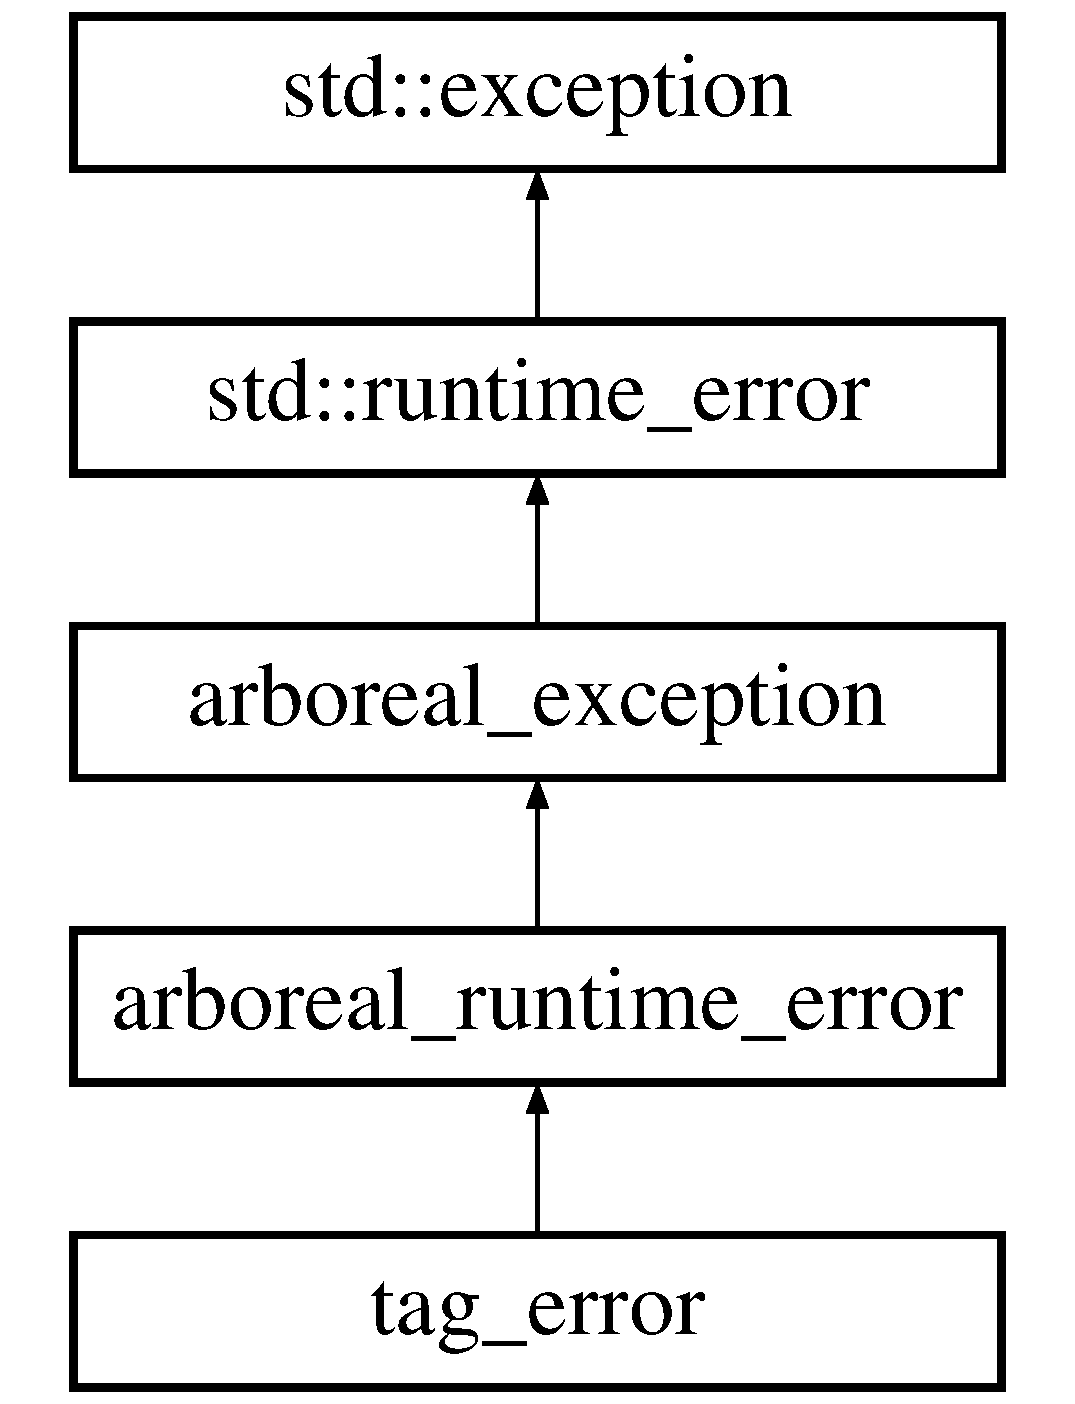
\includegraphics[height=4.000000cm]{classtag__error}
\end{center}
\end{figure}
\subsection*{Public Member Functions}
\begin{DoxyCompactItemize}
\item 
{\bfseries tag\+\_\+error} (const char $\ast$what, const char $\ast$where, const int ecode=99)\hypertarget{classtag__error_a49b7eb59916bbc065f7d79bbf31cb460}{}\label{classtag__error_a49b7eb59916bbc065f7d79bbf31cb460}

\item 
{\bfseries tag\+\_\+error} (const char $\ast$what, const string \&where, const int ecode=99)\hypertarget{classtag__error_abc7794a3cf421776f77b781b4bef9dfb}{}\label{classtag__error_abc7794a3cf421776f77b781b4bef9dfb}

\item 
{\bfseries tag\+\_\+error} (const string \&what, const string \&where, const int ecode=99)\hypertarget{classtag__error_afc103fa30ef508088c2cb4eda60837d2}{}\label{classtag__error_afc103fa30ef508088c2cb4eda60837d2}

\item 
{\bfseries tag\+\_\+error} (const string \&what, const char $\ast$where, const int ecode=99)\hypertarget{classtag__error_a70a4e7f9da04ca034f23e42ce1e95433}{}\label{classtag__error_a70a4e7f9da04ca034f23e42ce1e95433}

\end{DoxyCompactItemize}
\subsection*{Additional Inherited Members}


The documentation for this class was generated from the following files\+:\begin{DoxyCompactItemize}
\item 
Shared\+Headers/Arboreal\+\_\+\+Exceptions.\+h\item 
Shared\+C\+P\+P\+Files/Arboreal\+\_\+\+Exceptions.\+cpp\end{DoxyCompactItemize}

\hypertarget{classTagTree}{}\section{Tag\+Tree Class Reference}
\label{classTagTree}\index{Tag\+Tree@{Tag\+Tree}}
Inheritance diagram for Tag\+Tree\+:\begin{figure}[H]
\begin{center}
\leavevmode
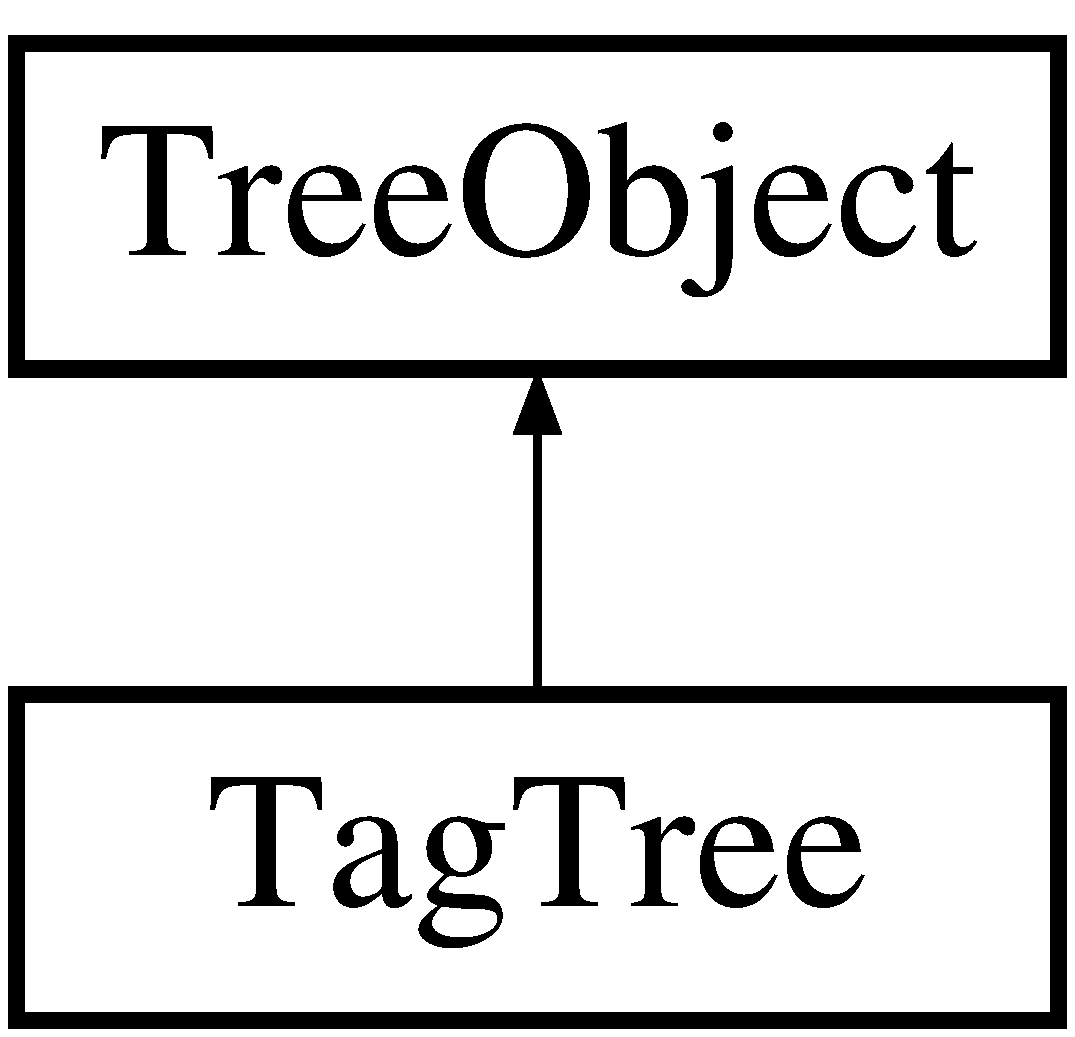
\includegraphics[height=2.000000cm]{classTagTree}
\end{center}
\end{figure}
\subsection*{Public Member Functions}
\begin{DoxyCompactItemize}
\item 
\mbox{\Hypertarget{classTagTree_a80b23fa47a18727a248c3db1e8b2ed83}\label{classTagTree_a80b23fa47a18727a248c3db1e8b2ed83}} 
{\bfseries Tag\+Tree} (string tag\+Name, Blk\+Num\+Type blknum, \mbox{\hyperlink{classPartitionManager}{Partition\+Manager}} $\ast$pm)
\item 
void \mbox{\hyperlink{classTagTree_ae316c2517c607547f02ce43b63a6316d}{write\+Out}} ()
\item 
\mbox{\Hypertarget{classTagTree_a2e72921ccc19667331c64d3d0100b269}\label{classTagTree_a2e72921ccc19667331c64d3d0100b269}} 
void {\bfseries read\+In} (unordered\+\_\+multimap$<$ string, \mbox{\hyperlink{classFileInfo}{File\+Info}} $\ast$$>$ $\ast$all\+Files, \mbox{\hyperlink{classRootTree}{Root\+Tree}} $\ast$root\+Tree)
\item 
\mbox{\Hypertarget{classTagTree_ad8108969f4d28b938e55c8339f19db35}\label{classTagTree_ad8108969f4d28b938e55c8339f19db35}} 
void {\bfseries del} ()
\end{DoxyCompactItemize}
\subsection*{Additional Inherited Members}


\subsection{Member Function Documentation}
\mbox{\Hypertarget{classTagTree_ae316c2517c607547f02ce43b63a6316d}\label{classTagTree_ae316c2517c607547f02ce43b63a6316d}} 
\index{Tag\+Tree@{Tag\+Tree}!write\+Out@{write\+Out}}
\index{write\+Out@{write\+Out}!Tag\+Tree@{Tag\+Tree}}
\subsubsection{\texorpdfstring{write\+Out()}{writeOut()}}
{\footnotesize\ttfamily void Tag\+Tree\+::write\+Out (\begin{DoxyParamCaption}{ }\end{DoxyParamCaption})\hspace{0.3cm}{\ttfamily [virtual]}}

Intended to write out the object to disk 

Implements \mbox{\hyperlink{classTreeObject_abf2bf88337bec961784b5dfeb9b795ed}{Tree\+Object}}.



The documentation for this class was generated from the following files\+:\begin{DoxyCompactItemize}
\item 
Trees.\+h\item 
Trees.\+cpp\end{DoxyCompactItemize}

\hypertarget{structtagTreeSuperBlock}{}\section{tag\+Tree\+Super\+Block Struct Reference}
\label{structtagTreeSuperBlock}\index{tag\+Tree\+Super\+Block@{tag\+Tree\+Super\+Block}}
\subsection*{Public Attributes}
\begin{DoxyCompactItemize}
\item 
\mbox{\Hypertarget{structtagTreeSuperBlock_a5fba4a1328640e6b41f4c3e8ca7ee804}\label{structtagTreeSuperBlock_a5fba4a1328640e6b41f4c3e8ca7ee804}} 
size\+\_\+t {\bfseries size}
\item 
\mbox{\Hypertarget{structtagTreeSuperBlock_ac2492d025873ac0d95921ee91acabe51}\label{structtagTreeSuperBlock_ac2492d025873ac0d95921ee91acabe51}} 
\mbox{\hyperlink{structindex}{Index}} {\bfseries last\+Entry}
\item 
\mbox{\Hypertarget{structtagTreeSuperBlock_ad7f50abf9a6efeee63037e73d0c349d9}\label{structtagTreeSuperBlock_ad7f50abf9a6efeee63037e73d0c349d9}} 
Blk\+Num\+Type {\bfseries start\+Block}
\end{DoxyCompactItemize}


The documentation for this struct was generated from the following file\+:\begin{DoxyCompactItemize}
\item 
types.\+h\end{DoxyCompactItemize}

\hypertarget{classTreeObject}{}\section{Tree\+Object Class Reference}
\label{classTreeObject}\index{Tree\+Object@{Tree\+Object}}
Inheritance diagram for Tree\+Object\+:\begin{figure}[H]
\begin{center}
\leavevmode
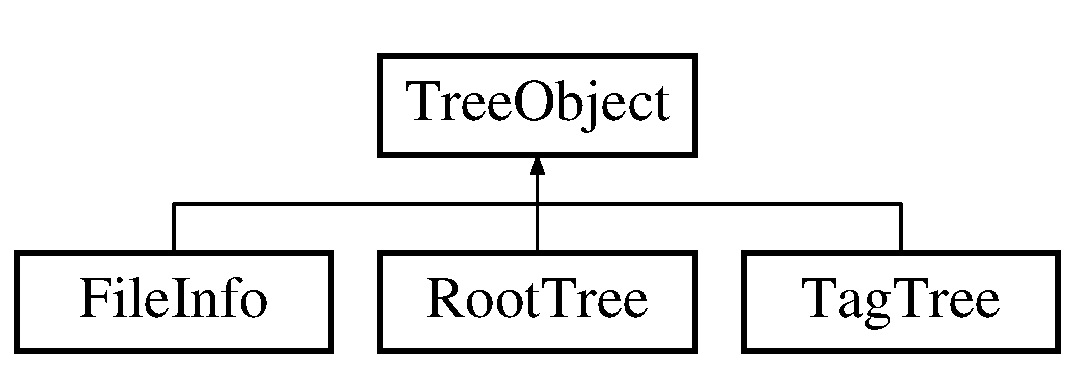
\includegraphics[height=2.000000cm]{d9/da2/classTreeObject}
\end{center}
\end{figure}
\subsection*{Public Member Functions}
\begin{DoxyCompactItemize}
\item 
\mbox{\hyperlink{classTreeObject_a1ef90156e6b45ddef28c59a89cd1097d}{Tree\+Object}} (string name, Blk\+Num\+Type blknum, \mbox{\hyperlink{classPartitionManager}{Partition\+Manager}} $\ast$pm)
\end{DoxyCompactItemize}
\begin{Indent}\textbf{ Accessor Functions}\par
\begin{DoxyCompactItemize}
\item 
string \mbox{\hyperlink{classTreeObject_a5216922ec0b98bcc375601db8d253770}{get\+\_\+name}} () const
\item 
Blk\+Num\+Type \mbox{\hyperlink{classTreeObject_af7841065fe85d0884341d72669185169}{get\+\_\+block\+\_\+number}} () const
\item 
\mbox{\hyperlink{structindex}{Index}} \mbox{\hyperlink{classTreeObject_ae0983a3ff99d413e22beaaac8d7b6d12}{get\+\_\+index}} (\mbox{\hyperlink{classTreeObject}{Tree\+Object}} $\ast$obj) const
\item 
\mbox{\hyperlink{structindex}{Index}} \mbox{\hyperlink{classTreeObject_a2d7c1a4c2d36c81110ccae09d9724125}{get\+\_\+last\+\_\+entry}} () const
\item 
Blk\+Num\+Type \mbox{\hyperlink{classTreeObject_a16153734dbee4adc99fa195715728c2f}{get\+\_\+start\+\_\+block}} () const
\item 
size\+\_\+t \mbox{\hyperlink{classTreeObject_a2a3dffe29aba8965c7977312c3721b50}{size}} () const
\item 
unordered\+\_\+map$<$ string, \mbox{\hyperlink{classTreeObject}{Tree\+Object}} $\ast$ $>$\+::iterator \mbox{\hyperlink{classTreeObject_af8bb5e54c0a13e1e0e5be409153ab6d8}{begin}} ()
\item 
unordered\+\_\+map$<$ string, \mbox{\hyperlink{classTreeObject}{Tree\+Object}} $\ast$ $>$\+::iterator \mbox{\hyperlink{classTreeObject_a2544e2976f3b75cd1f0230f5f908059c}{end}} ()
\item 
\mbox{\hyperlink{classTreeObject}{Tree\+Object}} $\ast$ \mbox{\hyperlink{classTreeObject_a6a7477c29a06a9896df549f83611252f}{find}} (string name) const
\item 
queue$<$ \mbox{\hyperlink{structindex}{Index}} $>$ $\ast$ \mbox{\hyperlink{classTreeObject_aa0900ad50c10023e4700f11218d30d7a}{get\+\_\+free\+\_\+spots}} ()
\end{DoxyCompactItemize}
\end{Indent}
\begin{Indent}\textbf{ Modifier Functions}\par
\begin{DoxyCompactItemize}
\item 
void \mbox{\hyperlink{classTreeObject_a8ae7e42502b4652102e0b3c4c4e1671b}{set\+\_\+name}} (string name)
\item 
void \mbox{\hyperlink{classTreeObject_af908239ff96a0f3064d0d8aefb58381b}{add\+\_\+index}} (\mbox{\hyperlink{classTreeObject}{Tree\+Object}} $\ast$obj, \mbox{\hyperlink{structindex}{Index}} \mbox{\hyperlink{structindex}{index}})
\item 
void \mbox{\hyperlink{classTreeObject_a2ec94bc9d2647275049ddf2a70b8510e}{set\+\_\+last\+\_\+entry}} (\mbox{\hyperlink{structindex}{Index}} \mbox{\hyperlink{structindex}{index}})
\item 
virtual void \mbox{\hyperlink{classTreeObject_af8cc57edba9f435b52ccf33cfbbb2fc6}{insert}} (string name, \mbox{\hyperlink{classTreeObject}{Tree\+Object}} $\ast$obj)
\item 
virtual void \mbox{\hyperlink{classTreeObject_a453b5df2a9ef7c6faad259900d574ee2}{erase}} (string name)
\item 
virtual void \mbox{\hyperlink{classTreeObject_a41ce6080e0df5adcea4b0a76d35af885}{insert\+\_\+addition}} (\mbox{\hyperlink{classTreeObject}{Tree\+Object}} $\ast$add)
\item 
virtual void \mbox{\hyperlink{classTreeObject_afcc4b3928d2b77ff080aa229a9706215}{insert\+\_\+deletion}} (\mbox{\hyperlink{classTreeObject}{Tree\+Object}} $\ast$\mbox{\hyperlink{classTreeObject_af390b7479aa972888e594c07a85740b6}{del}})
\end{DoxyCompactItemize}
\end{Indent}
\begin{Indent}\textbf{ Disk Functions}\par
\begin{DoxyCompactItemize}
\item 
virtual void \mbox{\hyperlink{classTreeObject_a63708d61353d83e3e03597394bb7aca0}{write\+\_\+out}} ()=0
\item 
virtual void \mbox{\hyperlink{classTreeObject_a722eb00e6782626281afc8eff92840a4}{read\+\_\+in}} (unordered\+\_\+multimap$<$ string, \mbox{\hyperlink{classFileInfo}{File\+Info}} $\ast$$>$ $\ast$all\+Files, \mbox{\hyperlink{classRootTree}{Root\+Tree}} $\ast$root\+Tree)=0
\item 
virtual void \mbox{\hyperlink{classTreeObject_af390b7479aa972888e594c07a85740b6}{del}} ()=0
\item 
void \mbox{\hyperlink{classTreeObject_a6b6f0a5c23577748b489652013fa1728}{increment\+\_\+allocate}} (\mbox{\hyperlink{structindex}{Index}} $\ast$\mbox{\hyperlink{structindex}{index}})
\item 
void \mbox{\hyperlink{classTreeObject_a86fbde9e7ee245385bf7ca7a8f355bd0}{increment\+\_\+follow}} (\mbox{\hyperlink{structindex}{Index}} $\ast$\mbox{\hyperlink{structindex}{index}})
\end{DoxyCompactItemize}
\end{Indent}
\subsection*{Protected Member Functions}
\begin{DoxyCompactItemize}
\item 
virtual void \mbox{\hyperlink{classTreeObject_a07f5f5de1cff0cfdc2372e81559f5181}{delete\+\_\+cont\+\_\+blocks}} (Blk\+Num\+Type blknum)
\end{DoxyCompactItemize}
\subsection*{Protected Attributes}
\begin{DoxyCompactItemize}
\item 
\mbox{\Hypertarget{classTreeObject_ac285793f5d7cba8069670210606c66c7}\label{classTreeObject_ac285793f5d7cba8069670210606c66c7}} 
queue$<$ \mbox{\hyperlink{classModification}{Modification}} $\ast$ $>$ \mbox{\hyperlink{classTreeObject_ac285793f5d7cba8069670210606c66c7}{\+\_\+modifications}}
\begin{DoxyCompactList}\small\item\em A collection of associated Modifications. \end{DoxyCompactList}\item 
\mbox{\Hypertarget{classTreeObject_a59effca19a3475c84496c7f82c856d38}\label{classTreeObject_a59effca19a3475c84496c7f82c856d38}} 
unordered\+\_\+map$<$ string, \mbox{\hyperlink{classTreeObject}{Tree\+Object}} $\ast$ $>$ \mbox{\hyperlink{classTreeObject_a59effca19a3475c84496c7f82c856d38}{\+\_\+my\+Tree}}
\begin{DoxyCompactList}\small\item\em A collection of contained Tree\+Objects. \end{DoxyCompactList}\item 
\mbox{\Hypertarget{classTreeObject_a368b410ed9b21c7106babf2ba93399b3}\label{classTreeObject_a368b410ed9b21c7106babf2ba93399b3}} 
string \mbox{\hyperlink{classTreeObject_a368b410ed9b21c7106babf2ba93399b3}{\+\_\+name}}
\begin{DoxyCompactList}\small\item\em name or value \end{DoxyCompactList}\item 
\mbox{\Hypertarget{classTreeObject_a17cfa5bde700978b4ec326909362bd2c}\label{classTreeObject_a17cfa5bde700978b4ec326909362bd2c}} 
Blk\+Num\+Type \mbox{\hyperlink{classTreeObject_a17cfa5bde700978b4ec326909362bd2c}{\+\_\+block\+Number}}
\begin{DoxyCompactList}\small\item\em Blocknumber of the superblock on disk. \end{DoxyCompactList}\item 
\mbox{\Hypertarget{classTreeObject_ae79eb5bd12c820b50f5d10c3f9b5dc66}\label{classTreeObject_ae79eb5bd12c820b50f5d10c3f9b5dc66}} 
unordered\+\_\+map$<$ \mbox{\hyperlink{classTreeObject}{Tree\+Object}} $\ast$, \mbox{\hyperlink{structindex}{Index}} $>$ \mbox{\hyperlink{classTreeObject_ae79eb5bd12c820b50f5d10c3f9b5dc66}{\+\_\+indeces}}
\begin{DoxyCompactList}\small\item\em location(s) of the superblock entry(ies) on disk \end{DoxyCompactList}\item 
\mbox{\Hypertarget{classTreeObject_a1418b7078e9fbb06506a310ad9417c52}\label{classTreeObject_a1418b7078e9fbb06506a310ad9417c52}} 
\mbox{\hyperlink{structindex}{Index}} \mbox{\hyperlink{classTreeObject_a1418b7078e9fbb06506a310ad9417c52}{\+\_\+last\+Entry}}
\begin{DoxyCompactList}\small\item\em Index of the last entry of data on disk. \end{DoxyCompactList}\item 
\mbox{\Hypertarget{classTreeObject_a5872ffdaa0c1a0cbf393da9a8a7657f3}\label{classTreeObject_a5872ffdaa0c1a0cbf393da9a8a7657f3}} 
Blk\+Num\+Type \mbox{\hyperlink{classTreeObject_a5872ffdaa0c1a0cbf393da9a8a7657f3}{\+\_\+start\+Block}}
\begin{DoxyCompactList}\small\item\em blocknumber of the start of this data on disk \end{DoxyCompactList}\item 
\mbox{\Hypertarget{classTreeObject_a0b2ab130a5b95945bbd81250f667d63b}\label{classTreeObject_a0b2ab130a5b95945bbd81250f667d63b}} 
\mbox{\hyperlink{classPartitionManager}{Partition\+Manager}} $\ast$ \mbox{\hyperlink{classTreeObject_a0b2ab130a5b95945bbd81250f667d63b}{\+\_\+my\+Partition\+Manager}}
\begin{DoxyCompactList}\small\item\em Associated \mbox{\hyperlink{classPartitionManager}{Partition\+Manager}}. \end{DoxyCompactList}\item 
\mbox{\Hypertarget{classTreeObject_a43defc5d87c903cdc3e36edc3323ef87}\label{classTreeObject_a43defc5d87c903cdc3e36edc3323ef87}} 
queue$<$ \mbox{\hyperlink{structindex}{Index}} $>$ {\bfseries \+\_\+free\+Spots}
\end{DoxyCompactItemize}


\subsection{Constructor \& Destructor Documentation}
\mbox{\Hypertarget{classTreeObject_a1ef90156e6b45ddef28c59a89cd1097d}\label{classTreeObject_a1ef90156e6b45ddef28c59a89cd1097d}} 
\index{Tree\+Object@{Tree\+Object}!Tree\+Object@{Tree\+Object}}
\index{Tree\+Object@{Tree\+Object}!Tree\+Object@{Tree\+Object}}
\subsubsection{\texorpdfstring{Tree\+Object()}{TreeObject()}}
{\footnotesize\ttfamily Tree\+Object\+::\+Tree\+Object (\begin{DoxyParamCaption}\item[{string}]{name,  }\item[{Blk\+Num\+Type}]{blknum,  }\item[{\mbox{\hyperlink{classPartitionManager}{Partition\+Manager}} $\ast$}]{pm }\end{DoxyParamCaption})}


\begin{DoxyParams}{Parameters}
{\em name} & name of this object \\
\hline
{\em blknum} & blocknumber of the superblock \\
\hline
{\em pm} & \mbox{\hyperlink{classPartitionManager}{Partition\+Manager}} object to be associated with this object \\
\hline
\end{DoxyParams}


\subsection{Member Function Documentation}
\mbox{\Hypertarget{classTreeObject_af908239ff96a0f3064d0d8aefb58381b}\label{classTreeObject_af908239ff96a0f3064d0d8aefb58381b}} 
\index{Tree\+Object@{Tree\+Object}!add\+\_\+index@{add\+\_\+index}}
\index{add\+\_\+index@{add\+\_\+index}!Tree\+Object@{Tree\+Object}}
\subsubsection{\texorpdfstring{add\+\_\+index()}{add\_index()}}
{\footnotesize\ttfamily void Tree\+Object\+::add\+\_\+index (\begin{DoxyParamCaption}\item[{\mbox{\hyperlink{classTreeObject}{Tree\+Object}} $\ast$}]{obj,  }\item[{\mbox{\hyperlink{structindex}{Index}}}]{index }\end{DoxyParamCaption})}

Add an index to \+\_\+indeces for the specified \mbox{\hyperlink{classTreeObject}{Tree\+Object}}. If the index already existed. nothing happpens 
\begin{DoxyParams}{Parameters}
{\em obj} & the object that the Index references to \\
\hline
{\em index} & the Index of obj \\
\hline
\end{DoxyParams}
\mbox{\Hypertarget{classTreeObject_af8bb5e54c0a13e1e0e5be409153ab6d8}\label{classTreeObject_af8bb5e54c0a13e1e0e5be409153ab6d8}} 
\index{Tree\+Object@{Tree\+Object}!begin@{begin}}
\index{begin@{begin}!Tree\+Object@{Tree\+Object}}
\subsubsection{\texorpdfstring{begin()}{begin()}}
{\footnotesize\ttfamily unordered\+\_\+map$<$ string, \mbox{\hyperlink{classTreeObject}{Tree\+Object}} $\ast$ $>$\+::iterator Tree\+Object\+::begin (\begin{DoxyParamCaption}{ }\end{DoxyParamCaption})}

\begin{DoxyReturn}{Returns}
An iterator to the beginning of the Tree\+Objects associated with this object 
\end{DoxyReturn}
\mbox{\Hypertarget{classTreeObject_af390b7479aa972888e594c07a85740b6}\label{classTreeObject_af390b7479aa972888e594c07a85740b6}} 
\index{Tree\+Object@{Tree\+Object}!del@{del}}
\index{del@{del}!Tree\+Object@{Tree\+Object}}
\subsubsection{\texorpdfstring{del()}{del()}}
{\footnotesize\ttfamily virtual void Tree\+Object\+::del (\begin{DoxyParamCaption}{ }\end{DoxyParamCaption})\hspace{0.3cm}{\ttfamily [pure virtual]}}

Will completely remove the \mbox{\hyperlink{classTreeObject}{Tree\+Object}}\textquotesingle{}s presence on disk 

Implemented in \mbox{\hyperlink{classRootTree_ac431dc04b767fc66791c251d8173650d}{Root\+Tree}}, \mbox{\hyperlink{classTagTree_ad8108969f4d28b938e55c8339f19db35}{Tag\+Tree}}, and \mbox{\hyperlink{classFileInfo_a2ca34d945ed1208f227a249ba72ee427}{File\+Info}}.

\mbox{\Hypertarget{classTreeObject_a07f5f5de1cff0cfdc2372e81559f5181}\label{classTreeObject_a07f5f5de1cff0cfdc2372e81559f5181}} 
\index{Tree\+Object@{Tree\+Object}!delete\+\_\+cont\+\_\+blocks@{delete\+\_\+cont\+\_\+blocks}}
\index{delete\+\_\+cont\+\_\+blocks@{delete\+\_\+cont\+\_\+blocks}!Tree\+Object@{Tree\+Object}}
\subsubsection{\texorpdfstring{delete\+\_\+cont\+\_\+blocks()}{delete\_cont\_blocks()}}
{\footnotesize\ttfamily void Tree\+Object\+::delete\+\_\+cont\+\_\+blocks (\begin{DoxyParamCaption}\item[{Blk\+Num\+Type}]{blknum }\end{DoxyParamCaption})\hspace{0.3cm}{\ttfamily [protected]}, {\ttfamily [virtual]}}

Will follow the chain of continuation blocks and free all of them 
\begin{DoxyParams}{Parameters}
{\em blknum} & will free the blknum and use it to follow the chain of continuation blocks \\
\hline
\end{DoxyParams}


Reimplemented in \mbox{\hyperlink{classFileInfo_a8c6b58cb9f7e9978064291ef81380e01}{File\+Info}}.

\mbox{\Hypertarget{classTreeObject_a2544e2976f3b75cd1f0230f5f908059c}\label{classTreeObject_a2544e2976f3b75cd1f0230f5f908059c}} 
\index{Tree\+Object@{Tree\+Object}!end@{end}}
\index{end@{end}!Tree\+Object@{Tree\+Object}}
\subsubsection{\texorpdfstring{end()}{end()}}
{\footnotesize\ttfamily unordered\+\_\+map$<$ string, \mbox{\hyperlink{classTreeObject}{Tree\+Object}} $\ast$ $>$\+::iterator Tree\+Object\+::end (\begin{DoxyParamCaption}{ }\end{DoxyParamCaption})}

\begin{DoxyReturn}{Returns}
An iterator to the end of the Tree\+Objects associated with this object 
\end{DoxyReturn}
\mbox{\Hypertarget{classTreeObject_a453b5df2a9ef7c6faad259900d574ee2}\label{classTreeObject_a453b5df2a9ef7c6faad259900d574ee2}} 
\index{Tree\+Object@{Tree\+Object}!erase@{erase}}
\index{erase@{erase}!Tree\+Object@{Tree\+Object}}
\subsubsection{\texorpdfstring{erase()}{erase()}}
{\footnotesize\ttfamily void Tree\+Object\+::erase (\begin{DoxyParamCaption}\item[{string}]{name }\end{DoxyParamCaption})\hspace{0.3cm}{\ttfamily [virtual]}}

Disassociate the given name from this object 
\begin{DoxyParams}{Parameters}
{\em name} & the name of the object to be erased. \\
\hline
\end{DoxyParams}

\begin{DoxyExceptions}{Exceptions}
{\em \mbox{\hyperlink{classarboreal__logic__error}{arboreal\+\_\+logic\+\_\+error}}} & \\
\hline
\end{DoxyExceptions}


Reimplemented in \mbox{\hyperlink{classFileInfo_ae058242283d3317eaf2b79428e6137f6}{File\+Info}}.

\mbox{\Hypertarget{classTreeObject_a6a7477c29a06a9896df549f83611252f}\label{classTreeObject_a6a7477c29a06a9896df549f83611252f}} 
\index{Tree\+Object@{Tree\+Object}!find@{find}}
\index{find@{find}!Tree\+Object@{Tree\+Object}}
\subsubsection{\texorpdfstring{find()}{find()}}
{\footnotesize\ttfamily \mbox{\hyperlink{classTreeObject}{Tree\+Object}} $\ast$ Tree\+Object\+::find (\begin{DoxyParamCaption}\item[{string}]{name }\end{DoxyParamCaption}) const}

Search \+\_\+my\+Tree for the specified name 
\begin{DoxyParams}{Parameters}
{\em name} & the name of the desired object \\
\hline
\end{DoxyParams}
\begin{DoxyReturn}{Returns}
a pointer to the object if found, 0 otherwise 
\end{DoxyReturn}
\mbox{\Hypertarget{classTreeObject_af7841065fe85d0884341d72669185169}\label{classTreeObject_af7841065fe85d0884341d72669185169}} 
\index{Tree\+Object@{Tree\+Object}!get\+\_\+block\+\_\+number@{get\+\_\+block\+\_\+number}}
\index{get\+\_\+block\+\_\+number@{get\+\_\+block\+\_\+number}!Tree\+Object@{Tree\+Object}}
\subsubsection{\texorpdfstring{get\+\_\+block\+\_\+number()}{get\_block\_number()}}
{\footnotesize\ttfamily Blk\+Num\+Type Tree\+Object\+::get\+\_\+block\+\_\+number (\begin{DoxyParamCaption}{ }\end{DoxyParamCaption}) const}

\begin{DoxyReturn}{Returns}
The blocknumber of the superblock 
\end{DoxyReturn}
\mbox{\Hypertarget{classTreeObject_aa0900ad50c10023e4700f11218d30d7a}\label{classTreeObject_aa0900ad50c10023e4700f11218d30d7a}} 
\index{Tree\+Object@{Tree\+Object}!get\+\_\+free\+\_\+spots@{get\+\_\+free\+\_\+spots}}
\index{get\+\_\+free\+\_\+spots@{get\+\_\+free\+\_\+spots}!Tree\+Object@{Tree\+Object}}
\subsubsection{\texorpdfstring{get\+\_\+free\+\_\+spots()}{get\_free\_spots()}}
{\footnotesize\ttfamily queue$<$ \mbox{\hyperlink{structindex}{Index}} $>$ $\ast$ Tree\+Object\+::get\+\_\+free\+\_\+spots (\begin{DoxyParamCaption}{ }\end{DoxyParamCaption})}

\begin{DoxyReturn}{Returns}
a pointer to the queue of empty spaces where new entries can be added 
\end{DoxyReturn}
\mbox{\Hypertarget{classTreeObject_ae0983a3ff99d413e22beaaac8d7b6d12}\label{classTreeObject_ae0983a3ff99d413e22beaaac8d7b6d12}} 
\index{Tree\+Object@{Tree\+Object}!get\+\_\+index@{get\+\_\+index}}
\index{get\+\_\+index@{get\+\_\+index}!Tree\+Object@{Tree\+Object}}
\subsubsection{\texorpdfstring{get\+\_\+index()}{get\_index()}}
{\footnotesize\ttfamily \mbox{\hyperlink{structindex}{Index}} Tree\+Object\+::get\+\_\+index (\begin{DoxyParamCaption}\item[{\mbox{\hyperlink{classTreeObject}{Tree\+Object}} $\ast$}]{obj }\end{DoxyParamCaption}) const}

Searches for obj and returns the Index of obj on disk, if found 
\begin{DoxyParams}{Parameters}
{\em obj} & object whose position is desired \\
\hline
\end{DoxyParams}
\begin{DoxyReturn}{Returns}
The Index of obj on disk, 
\end{DoxyReturn}

\begin{DoxyExceptions}{Exceptions}
{\em \mbox{\hyperlink{classarboreal__logic__error}{arboreal\+\_\+logic\+\_\+error}}} & \\
\hline
\end{DoxyExceptions}
\mbox{\Hypertarget{classTreeObject_a2d7c1a4c2d36c81110ccae09d9724125}\label{classTreeObject_a2d7c1a4c2d36c81110ccae09d9724125}} 
\index{Tree\+Object@{Tree\+Object}!get\+\_\+last\+\_\+entry@{get\+\_\+last\+\_\+entry}}
\index{get\+\_\+last\+\_\+entry@{get\+\_\+last\+\_\+entry}!Tree\+Object@{Tree\+Object}}
\subsubsection{\texorpdfstring{get\+\_\+last\+\_\+entry()}{get\_last\_entry()}}
{\footnotesize\ttfamily \mbox{\hyperlink{structindex}{Index}} Tree\+Object\+::get\+\_\+last\+\_\+entry (\begin{DoxyParamCaption}{ }\end{DoxyParamCaption}) const}

Find the Index of the last entry for this object on disk \begin{DoxyReturn}{Returns}
Index of the last entry on disk 
\end{DoxyReturn}
\mbox{\Hypertarget{classTreeObject_a5216922ec0b98bcc375601db8d253770}\label{classTreeObject_a5216922ec0b98bcc375601db8d253770}} 
\index{Tree\+Object@{Tree\+Object}!get\+\_\+name@{get\+\_\+name}}
\index{get\+\_\+name@{get\+\_\+name}!Tree\+Object@{Tree\+Object}}
\subsubsection{\texorpdfstring{get\+\_\+name()}{get\_name()}}
{\footnotesize\ttfamily string Tree\+Object\+::get\+\_\+name (\begin{DoxyParamCaption}{ }\end{DoxyParamCaption}) const}

\begin{DoxyReturn}{Returns}
The name 
\end{DoxyReturn}
\mbox{\Hypertarget{classTreeObject_a16153734dbee4adc99fa195715728c2f}\label{classTreeObject_a16153734dbee4adc99fa195715728c2f}} 
\index{Tree\+Object@{Tree\+Object}!get\+\_\+start\+\_\+block@{get\+\_\+start\+\_\+block}}
\index{get\+\_\+start\+\_\+block@{get\+\_\+start\+\_\+block}!Tree\+Object@{Tree\+Object}}
\subsubsection{\texorpdfstring{get\+\_\+start\+\_\+block()}{get\_start\_block()}}
{\footnotesize\ttfamily Blk\+Num\+Type Tree\+Object\+::get\+\_\+start\+\_\+block (\begin{DoxyParamCaption}{ }\end{DoxyParamCaption}) const}

\begin{DoxyReturn}{Returns}
The start block of data for this object 
\end{DoxyReturn}
\mbox{\Hypertarget{classTreeObject_a6b6f0a5c23577748b489652013fa1728}\label{classTreeObject_a6b6f0a5c23577748b489652013fa1728}} 
\index{Tree\+Object@{Tree\+Object}!increment\+\_\+allocate@{increment\+\_\+allocate}}
\index{increment\+\_\+allocate@{increment\+\_\+allocate}!Tree\+Object@{Tree\+Object}}
\subsubsection{\texorpdfstring{increment\+\_\+allocate()}{increment\_allocate()}}
{\footnotesize\ttfamily void Tree\+Object\+::increment\+\_\+allocate (\begin{DoxyParamCaption}\item[{\mbox{\hyperlink{structindex}{Index}} $\ast$}]{index }\end{DoxyParamCaption})}

Will increment the Index passed and allocate blocks if necessary to do so 
\begin{DoxyParams}{Parameters}
{\em index} & the Index to be incremented \\
\hline
\end{DoxyParams}
\mbox{\Hypertarget{classTreeObject_a86fbde9e7ee245385bf7ca7a8f355bd0}\label{classTreeObject_a86fbde9e7ee245385bf7ca7a8f355bd0}} 
\index{Tree\+Object@{Tree\+Object}!increment\+\_\+follow@{increment\+\_\+follow}}
\index{increment\+\_\+follow@{increment\+\_\+follow}!Tree\+Object@{Tree\+Object}}
\subsubsection{\texorpdfstring{increment\+\_\+follow()}{increment\_follow()}}
{\footnotesize\ttfamily void Tree\+Object\+::increment\+\_\+follow (\begin{DoxyParamCaption}\item[{\mbox{\hyperlink{structindex}{Index}} $\ast$}]{index }\end{DoxyParamCaption})}

Will increment the Index passed but only follow the chain of already allocated blocks 
\begin{DoxyParams}{Parameters}
{\em index} & the Index to be incremented \\
\hline
\end{DoxyParams}
\mbox{\Hypertarget{classTreeObject_af8cc57edba9f435b52ccf33cfbbb2fc6}\label{classTreeObject_af8cc57edba9f435b52ccf33cfbbb2fc6}} 
\index{Tree\+Object@{Tree\+Object}!insert@{insert}}
\index{insert@{insert}!Tree\+Object@{Tree\+Object}}
\subsubsection{\texorpdfstring{insert()}{insert()}}
{\footnotesize\ttfamily void Tree\+Object\+::insert (\begin{DoxyParamCaption}\item[{string}]{name,  }\item[{\mbox{\hyperlink{classTreeObject}{Tree\+Object}} $\ast$}]{obj }\end{DoxyParamCaption})\hspace{0.3cm}{\ttfamily [virtual]}}

Associate a \mbox{\hyperlink{classTreeObject}{Tree\+Object}} with this object 
\begin{DoxyParams}{Parameters}
{\em name} & name of the object, mangled if inserting a \mbox{\hyperlink{classFileInfo}{File\+Info}} \\
\hline
{\em obj} & the object to be inserted \\
\hline
\end{DoxyParams}

\begin{DoxyExceptions}{Exceptions}
{\em \mbox{\hyperlink{classtag__error}{tag\+\_\+error}}} & \\
\hline
\end{DoxyExceptions}
\begin{DoxySeeAlso}{See also}
\mbox{\hyperlink{classFileInfo_ad93a84b63e417b07aa68b619051ab746}{File\+Info\+::insert()}} 
\end{DoxySeeAlso}


Reimplemented in \mbox{\hyperlink{classFileInfo_ad93a84b63e417b07aa68b619051ab746}{File\+Info}}.

\mbox{\Hypertarget{classTreeObject_a41ce6080e0df5adcea4b0a76d35af885}\label{classTreeObject_a41ce6080e0df5adcea4b0a76d35af885}} 
\index{Tree\+Object@{Tree\+Object}!insert\+\_\+addition@{insert\+\_\+addition}}
\index{insert\+\_\+addition@{insert\+\_\+addition}!Tree\+Object@{Tree\+Object}}
\subsubsection{\texorpdfstring{insert\+\_\+addition()}{insert\_addition()}}
{\footnotesize\ttfamily void Tree\+Object\+::insert\+\_\+addition (\begin{DoxyParamCaption}\item[{\mbox{\hyperlink{classTreeObject}{Tree\+Object}} $\ast$}]{add }\end{DoxyParamCaption})\hspace{0.3cm}{\ttfamily [virtual]}}

Add an \mbox{\hyperlink{classAddition}{Addition}} to the list of Modifications so that it can be written out later. Note\+: Do not call this on a \mbox{\hyperlink{classFileInfo}{File\+Info}}. 
\begin{DoxyParams}{Parameters}
{\em add} & the object that was previously inserted to this object which will be added to the list of Modifications \\
\hline
\end{DoxyParams}
\begin{DoxySeeAlso}{See also}
File\+System\+::write\+\_\+out() \mbox{\hyperlink{classTreeObject_af8cc57edba9f435b52ccf33cfbbb2fc6}{Tree\+Object\+::insert()}} 
\end{DoxySeeAlso}


Reimplemented in \mbox{\hyperlink{classFileInfo_a7f788f31521c535646eebfa9959bbb24}{File\+Info}}.

\mbox{\Hypertarget{classTreeObject_afcc4b3928d2b77ff080aa229a9706215}\label{classTreeObject_afcc4b3928d2b77ff080aa229a9706215}} 
\index{Tree\+Object@{Tree\+Object}!insert\+\_\+deletion@{insert\+\_\+deletion}}
\index{insert\+\_\+deletion@{insert\+\_\+deletion}!Tree\+Object@{Tree\+Object}}
\subsubsection{\texorpdfstring{insert\+\_\+deletion()}{insert\_deletion()}}
{\footnotesize\ttfamily void Tree\+Object\+::insert\+\_\+deletion (\begin{DoxyParamCaption}\item[{\mbox{\hyperlink{classTreeObject}{Tree\+Object}} $\ast$}]{del }\end{DoxyParamCaption})\hspace{0.3cm}{\ttfamily [virtual]}}

Add a \mbox{\hyperlink{classDeletion}{Deletion}} to the list of Modifications so that it can be written out later. Note\+: Do not call this on a \mbox{\hyperlink{classFileInfo}{File\+Info}}. 
\begin{DoxyParams}{Parameters}
{\em del} & the object that was previously erased from this object which will be added to the list of Modifications \\
\hline
\end{DoxyParams}
\begin{DoxySeeAlso}{See also}
File\+System\+::write\+\_\+out() \mbox{\hyperlink{classTreeObject_a453b5df2a9ef7c6faad259900d574ee2}{Tree\+Object\+::erase()}} 
\end{DoxySeeAlso}


Reimplemented in \mbox{\hyperlink{classFileInfo_a278136b1d68f55dc56a4be807076fc0d}{File\+Info}}.

\mbox{\Hypertarget{classTreeObject_a722eb00e6782626281afc8eff92840a4}\label{classTreeObject_a722eb00e6782626281afc8eff92840a4}} 
\index{Tree\+Object@{Tree\+Object}!read\+\_\+in@{read\+\_\+in}}
\index{read\+\_\+in@{read\+\_\+in}!Tree\+Object@{Tree\+Object}}
\subsubsection{\texorpdfstring{read\+\_\+in()}{read\_in()}}
{\footnotesize\ttfamily virtual void Tree\+Object\+::read\+\_\+in (\begin{DoxyParamCaption}\item[{unordered\+\_\+multimap$<$ string, \mbox{\hyperlink{classFileInfo}{File\+Info}} $\ast$$>$ $\ast$}]{all\+Files,  }\item[{\mbox{\hyperlink{classRootTree}{Root\+Tree}} $\ast$}]{root\+Tree }\end{DoxyParamCaption})\hspace{0.3cm}{\ttfamily [pure virtual]}}

Will read in all object data from disk 
\begin{DoxyParams}{Parameters}
{\em all\+Files} & a pointer to the map of all files \\
\hline
{\em root\+Tree} & a pointer to the root tree \\
\hline
\end{DoxyParams}


Implemented in \mbox{\hyperlink{classRootTree_a658eed78be67e890de2283af960dc532}{Root\+Tree}}, \mbox{\hyperlink{classTagTree_af86ee6713fa03c3909e04608512b8b62}{Tag\+Tree}}, and \mbox{\hyperlink{classFileInfo_a2bf60d4be97347f3d7a15cf839afca7d}{File\+Info}}.

\mbox{\Hypertarget{classTreeObject_a2ec94bc9d2647275049ddf2a70b8510e}\label{classTreeObject_a2ec94bc9d2647275049ddf2a70b8510e}} 
\index{Tree\+Object@{Tree\+Object}!set\+\_\+last\+\_\+entry@{set\+\_\+last\+\_\+entry}}
\index{set\+\_\+last\+\_\+entry@{set\+\_\+last\+\_\+entry}!Tree\+Object@{Tree\+Object}}
\subsubsection{\texorpdfstring{set\+\_\+last\+\_\+entry()}{set\_last\_entry()}}
{\footnotesize\ttfamily void Tree\+Object\+::set\+\_\+last\+\_\+entry (\begin{DoxyParamCaption}\item[{\mbox{\hyperlink{structindex}{Index}}}]{index }\end{DoxyParamCaption})}

Set the last Index for the last entry belonging to this object on disk 
\begin{DoxyParams}{Parameters}
{\em index} & The last Index \\
\hline
\end{DoxyParams}
\mbox{\Hypertarget{classTreeObject_a8ae7e42502b4652102e0b3c4c4e1671b}\label{classTreeObject_a8ae7e42502b4652102e0b3c4c4e1671b}} 
\index{Tree\+Object@{Tree\+Object}!set\+\_\+name@{set\+\_\+name}}
\index{set\+\_\+name@{set\+\_\+name}!Tree\+Object@{Tree\+Object}}
\subsubsection{\texorpdfstring{set\+\_\+name()}{set\_name()}}
{\footnotesize\ttfamily void Tree\+Object\+::set\+\_\+name (\begin{DoxyParamCaption}\item[{string}]{name }\end{DoxyParamCaption})}

Set the name 
\begin{DoxyParams}{Parameters}
{\em name} & The new name \\
\hline
\end{DoxyParams}
\mbox{\Hypertarget{classTreeObject_a2a3dffe29aba8965c7977312c3721b50}\label{classTreeObject_a2a3dffe29aba8965c7977312c3721b50}} 
\index{Tree\+Object@{Tree\+Object}!size@{size}}
\index{size@{size}!Tree\+Object@{Tree\+Object}}
\subsubsection{\texorpdfstring{size()}{size()}}
{\footnotesize\ttfamily size\+\_\+t Tree\+Object\+::size (\begin{DoxyParamCaption}{ }\end{DoxyParamCaption}) const}

\begin{DoxyReturn}{Returns}
The size of \+\_\+my\+Tree 
\end{DoxyReturn}
\mbox{\Hypertarget{classTreeObject_a63708d61353d83e3e03597394bb7aca0}\label{classTreeObject_a63708d61353d83e3e03597394bb7aca0}} 
\index{Tree\+Object@{Tree\+Object}!write\+\_\+out@{write\+\_\+out}}
\index{write\+\_\+out@{write\+\_\+out}!Tree\+Object@{Tree\+Object}}
\subsubsection{\texorpdfstring{write\+\_\+out()}{write\_out()}}
{\footnotesize\ttfamily virtual void Tree\+Object\+::write\+\_\+out (\begin{DoxyParamCaption}{ }\end{DoxyParamCaption})\hspace{0.3cm}{\ttfamily [pure virtual]}}

Intended to write out the object to disk 

Implemented in \mbox{\hyperlink{classRootTree_ad6eefe5d46ee37b3725799897a78c2dd}{Root\+Tree}}, \mbox{\hyperlink{classTagTree_adf13e01b25991ecfef1ad958e02c07fe}{Tag\+Tree}}, and \mbox{\hyperlink{classFileInfo_a8e835f000ddfd0f1097ccfa7e7801a09}{File\+Info}}.



The documentation for this class was generated from the following files\+:\begin{DoxyCompactItemize}
\item 
Filesystem/\+Daemon\+Dependancies/\+Trees/Trees.\+h\item 
Filesystem/\+Daemon\+Dependancies/\+Trees/Trees.\+cpp\end{DoxyCompactItemize}

%--- End generated contents ---

% Index
\backmatter
\newpage
\phantomsection
\clearemptydoublepage
\addcontentsline{toc}{chapter}{Index}
\printindex

\end{document}
